\section{Rete neurale}
\label{Rete neurale}

La libreria utilizzata per sviluppare la Rete neurale \`e stata \textit{ConvNetJS}. L'aspetto positivo di tale scelta \`e stata la semplicit\`a nell'utilizzo del linguaggio javascript; l'aspetto negativo ha riguardato la totale mancanza di mantenibilit\`a della libreria stessa che comporta la scarsit\`a di esempi applicativi, oltre alla documentazione ufficiale, che costringono lo sviluppatore ad una ricerca approfondita personale in un ambiente ove lo nozioni si presentano scarse e a continue prove per verificare la validit\`a del codice prodotto.
\begin{figure}[H]
\centering
	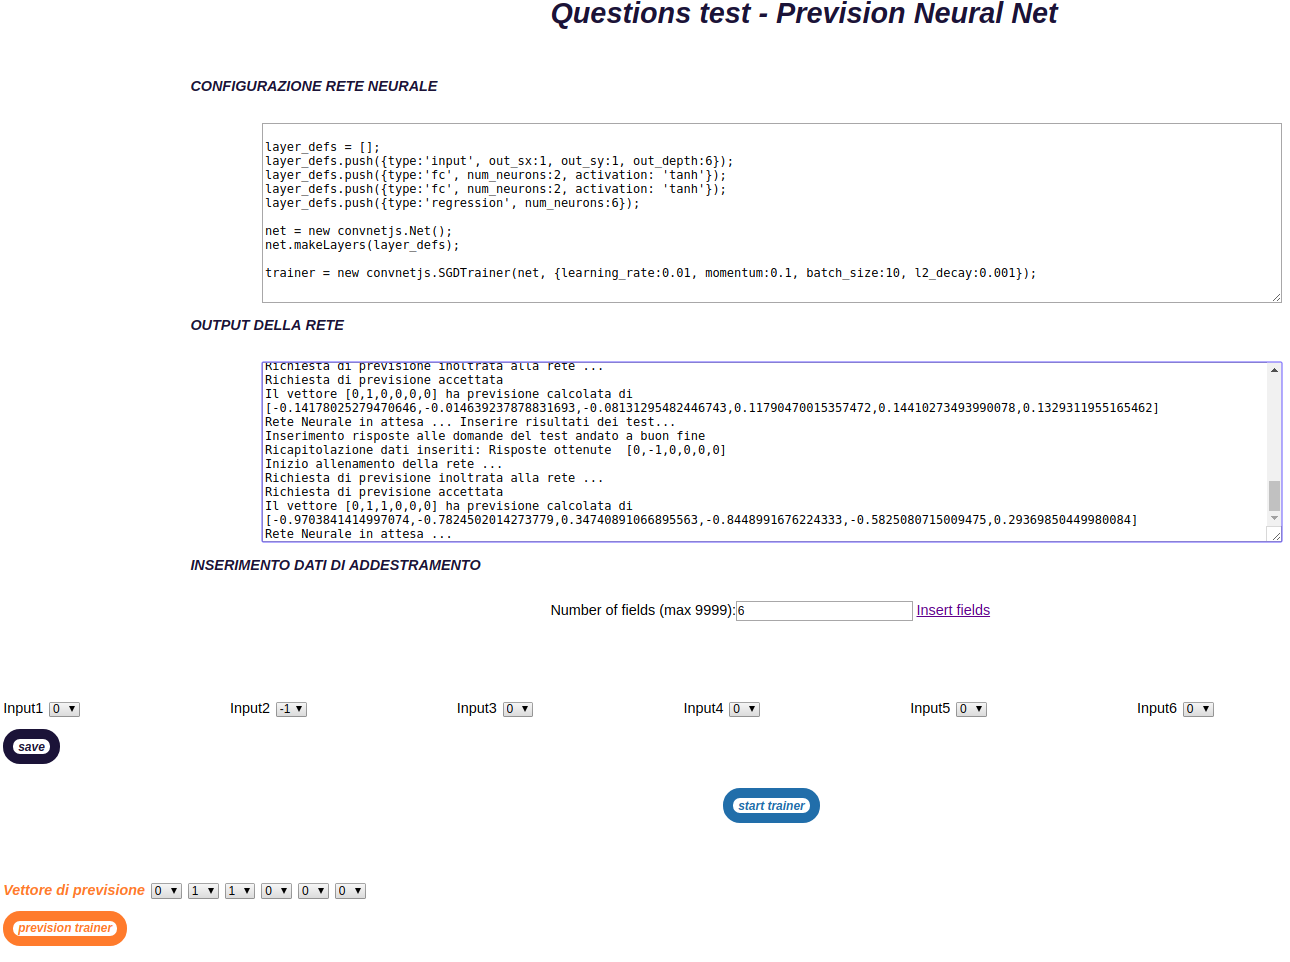
\includegraphics[width=1\linewidth]{./image/GUI-rete-neurale.png}
	\caption{Interfaccia utente della Rete neurale di prova.}
\end{figure}
\noindent
Durante il periodo 24/05 - 31/05 mi sono occupata dello sviluppo di una Rete neurale in grado di ricevere in input un training set di dimensione 6 e di restituire una previsione sui dati di apprendimento ricevuti.
\noindent
Il problema che la rete mira ad analizzare \`e quello discusso nel precedente capitolo \textit{Analisi dei dati di probabilit\`a}
\\\\
Per agevolare l'apprendimento della rete, ed ottenere delle previsioni stabili mi sono occupata di implementare due metodi di generazione randomica di dati in modo da far apprendere massicciamente la stessa.
Il dato prodotto consiste in un vettore di 6 elementi, composto da  -1, 0 e 1 con il seguente criterio:
\begin{itemize}
\item \textbf{-1}: la domanda x \`e stata posta al candidato che ha risposto in maniera errata;
\item \textbf{0}: la domanda x non \`e stata posta al candidato;
\item \textbf{1}: la domanda x \`e stata posta al candidato che ha saputo rispondere correttamente.
\end{itemize}
\noindent
Il primo metodo che ho sviluppato si occupa di generare un vettore di dati di apprendimento basandosi esclusivamente su come le domande sono interconnesse tra di loro (grazie all'uso di un grafo della conoscenza costruito ad hoc); il secondo metodo ripropone quanto perseguito dal primo metodo con il valore aggiunto di generazione di un profilo randomico di un candidato, che tiene conto della  probabilit\`a di risposta ad una domande seguendo la formula P(A)= $\frac{1}{3}+\frac{1}{6}P(S_1)+\frac{2}{3}P(S_2)$.

\subsection{Test effettuati}
\label{Test effettuati}

Alcune decisioni che ho preso durante la scelta dell'architettura della rete riguardano i seguenti settori:
\begin{enumerate}
\item Una rete neurale non deve, per fornire dei dati attendibili, possedere un numero di neuroni troppo elevato rispetto al trainset effettuato; altrimenti la previsione  ritornerebbe l'identit\`a del vettore di input della stessa, come conseguenza diretta della capacit\`a troppo elevata di immagazzinare dati.
\item I layers, ho deciso, di allenarli mediante tecnica di regressione, che permette l'inserimento in input di una funzione obiettivo e l'ottenimento di un risultato, in output, anche in virgola mobile e composto di tanti elementi quanti sono i neuroni di regressione dichiarati. Per la mia rete di prova \`e necessario dichiarare  6 neuroni in regressione perch\`e l'output, appunto, che ci si aspetta dal sistema \`e di 6 elementi.
\item Per costruire un dataset di dati consistente che permettesse alla rete di imparare qualcosa ho costruito un grafo della conoscenza con lo scopo di mettere in relazione degli argomenti che coinvolgono uno o pi\`u domande.
\begin{figure}[H]
\centering
	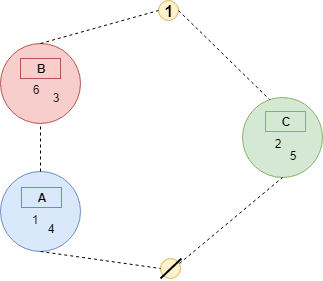
\includegraphics[width=0.60\linewidth]{./image/grafo_trainset.png}
	\caption{Grafo rappresentante le relazioni esistenti tra il set di domande di prova.}
\end{figure}
\noindent
Per svolgere l'apprendimento ogni vettore, facente parte del dataset, viene dato in pasto alla rete che a sua volta provvede alla sua assimilazione come conoscenza mediante la tecnica dell'autoencoder, ovvero la rete impara il vettore riducendone lo spazio occupato.
\item Per creare il dataset ho ritenuto sufficiente generare \textit{2000} vettori di risposta in modo da compiere in maniera esaustivo l'apprendimento della rete.
\end{enumerate}
\noindent
Il vettore passato in input per svolgere le previsioni \`e \textit{[0,0,0,0,0,0]},\textit{[0,0,1,0,1,0]} e \textit{[0,0,-1,0,0,0]}\\
Le aspettative riguardano la previsione di risposta di un candidato
\noindent. 
Di seguito riporto quanto \`e stato rilevato in fase di test.

\subsubsection{Architettura  della rete: 4 neuroni per ciascuno dei 2 layers}
\label{Configurazione della rete: 4 neuroni per ciascuno dei 2 layers}

Architettura  della rete utilizzata:\\
\begin{verbatim}layer_defs = [];
layer_defs.push({type:'input', out_sx:1, out_sy:1, out_depth:6});
layer_defs.push({type:'fc', num_neurons:4, activation: 'tanh'});
layer_defs.push({type:'fc', num_neurons:4, activation: 'tanh'});
layer_defs.push({type:'regression', num_neurons:6});

net = new convnetjs.Net();
net.makeLayers(layer_defs);

trainer = new convnetjs.SGDTrainer(net, {learning_rate:0.01,
 momentum:0.1, batch_size:10, l2_decay:0.001});
\end{verbatim}
\noindent
I layers utilizzati sono 2 e compositi da 4 neuroni.

\paragraph{Training set standard a 4 neuroni per ciascuno dei 2 layers}\mbox{}
\label{Training set standard a 4 neuroni per ciascuno dei 2 layers}
\\
\noindent
\begin{itemize}
\item \begin{verbatim}Il vettore [0,0,0,0,0,0] ha previsione calcolata di [-0.021598804903572744,-0.1372509042342871,0.06611969158456255
,0.018121335417653706,-0.11264571886853292,0.17520370837747462]\end{verbatim}
Appaiono in relazione le domande 1, 2, 5 e 3, 4, 6.\\
Gli scostamenti tra le coppie 2, 5 e 3, 6 sono consistenti con quelle che sono le relazioni di dipendenza, invece 1, 4 ha una differenza di 0.016 circa che parte da qualche millesimo fino 0.5
Le domande 3 e 6 si dovrebbero presentare con una positivit\`a inferiore rispetto a 1 e 4; nel test in analisi questo non viene rispettato da nessuna delle coppie in analisi per differenze che vanno da qualche millesimo fino a 0.018 circa.
\paragraph{Osservazioni}\mbox{}
\label{Osservazioni su rete a 4 neuroni per ciascuno dei 2 layers}
\\\\
\noindent
L'architettura testata si compone di 4 neuroni a layer su una base di 2000 test correndo il rischio di avere una rete che apprende troppo e come effetto negativo "veda" addirittura cose che non esistono. A prova di ci\`o sono i risultati non conformi alle attese.
Dunque mi fermo qui con il test di tale architettura e riducendone il numero di neuroni presenti in ciascun layers e/o il numero di layers presenti.\\

Le nuove architetture su cui ho effettuato i test sono esposte nei paragrafi seguenti.

\subsubsection{Architettura della rete a 2 neuroni per ciascuno dei 2 layers}
\label{Architettura della rete a 2 neuroni per ciascuno dei 2 layers}
Architettura  della rete utilizzata:\\
\begin{verbatim}layer_defs = [];
layer_defs.push({type:'input', out_sx:1, out_sy:1, out_depth:6});
layer_defs.push({type:'fc', num_neurons:2, activation: 'tanh'});
layer_defs.push({type:'fc', num_neurons:2, activation: 'tanh'});
layer_defs.push({type:'regression', num_neurons:6});

net = new convnetjs.Net();
net.makeLayers(layer_defs);

trainer = new convnetjs.SGDTrainer(net, {learning_rate:0.01,
 momentum:0.1, batch_size:10, l2_decay:0.001});
\end{verbatim}
\noindent
I layers utilizzati sono 2 compositi da 2 neuroni.

\paragraph{Training set standard su rete a 2 neuroni per ciascuno dei 2 layers}\mbox{}
\label{Training set standard su rete a 2 neuroni per ciascuno dei 2 layers}
\\
\noindent
\begin{itemize}
\item \begin{verbatim}[Il vettore [0,0,0,0,0,0] ha previsione calcolata di
[0.31232372051574936,0.7253754889487585,-0.5051208979797573,
0.32075742158673093,0.7324947496336937,-0.4348299972940168]
\end{verbatim}
Appaiono in relazione le domande 1, 2, 4, 5 e 3, 6.\\
Gli scostamenti tra le coppie 1, 4 e 3, 6  e 2, 5 sono consistenti con quelle che sono le relazioni di dipendenza fra le domande.
Le domande 3 e 6 si dovrebbero presentare con una positivit\`a inferiore rispetto a 1 e 4; in questo test la regola viene rispettata pienamente.\\
Dai dati della previsione si nota come il candidato ha una buona probabilit\`a di saper rispondere alla coppia 1 e 4, e ancora pi\`u elevata di saper rispondere correttamente alla coppia 2 e 5; molto bassa di saper rispondere correttamente alle 3 e 6 che sono, appunto, di una difficolt\`a maggiore rispetto alla coppia 1 e 4.

\item \begin{verbatim}Il vettore [0,0,1,0,1,0] ha previsione calcolata di
[0.5123144717131076,0.9123354449531641,0.2837937822420923,
0.46449868699771607,0.9029832167165894,0.3227303792035435]
\end{verbatim}
Appaiono in relazione le domande 1, 2, 3  4, 5, 6.\\
Gli scostamenti tra le coppie 1, 4 e 3, 6  e 2, 5 sono consistenti con quelle che sono le relazioni di dipendenza fra le domande.
Le domande 3 e 6 si dovrebbero presentare con una positivit\`a inferiore rispetto a 1 e 4; in questo test la regola viene rispettata pienamente.\\
Dai dati della previsione si nota come il candidato ha un'ottima probabilit\`a di saper rispondere alla coppia 2 e 5 (come imposto dal vettore previsione), buona di saper rispondere alla coppie 3 e 6 (come imposto dal vettore previsione) e pi\`u che buona  di saper rispondere alle 1 e 4, che sono di una semplicit\`a pi\`u elevata rispetto alla 3 e 4.
\end{itemize}

\item \begin{verbatim}Il vettore [0,0,-1,0,0,0] ha previsione calcolata di
[0.3698539826215957,0.288907514487717,-0.8504159455662308,
0.3663192502433841,0.2937448801761998,-0.7845589473185985]
\end{verbatim}
Appaiono in relazione le domande 1, 2, 4, 5 e 3, 6.\\
Gli scostamenti tra le coppie 1, 4 e 3, 6  e 2, 5 sono consistenti con quelle che sono le relazioni di dipendenza fra le domande.
Le domande 3 e 6 si dovrebbero presentare con una positivit\`a inferiore rispetto a 1 e 4; in questo test la regola viene rispettata pienamente.\\
Dai dati della previsione si nota come il candidato ha una discreta probabilit\`a di saper rispondere alla coppia 2 e 5, un p\`o meglio di saper rispondere alla coppie 1 e 4 e pi\`u di non saper saper rispondere alle 3 e 6 (come imposto dal vettore previsione).
\end{itemize}

\paragraph{Training set con generazione del profilo di un candidato e calcolo delle probabilit\`a di risposta a 2 neuroni per ciascuno dei 2 layers}\mbox{}
\label{Training set con generazione del profilo di un candidato e calcolo delle probabilita di risposta a 2 neuroni per ciascuno dei 2 layers}
\\
\noindent
\begin{itemize}
\item \begin{verbatim}Il vettore [0,0,0,0,0,0] ha previsione calcolata di
[0.057781303506280995,0.0513731100126314,-0.06600467867066256,
0.029940883111932555,-0.019564515397168573,-0.09570617900597932]
\end{verbatim}
Appaiono in relazione le domande 1, 2, 4 e 3, 5, 6.\\
Gli scostamenti tra la coppia 1, 4 e 3, 6 sono consistenti con  quelle che sono le relazioni di dipendenza fra le domande; invece per la coppia 2 e 5 i segni sono opposti con una differenza di 0.024.
Le domande 3 e 6 si dovrebbero presentare con una positivit\`a inferiore rispetto a 1 e 4, la regola viene rispettata pienamente. Le anomalie riscontrate sono da ricondurre alla natura del vettore di training che si basa sul calcolo della probabilit\`a di una risposta che sul grafo della conoscenza.

\item \begin{verbatim}Il vettore [0,0,1,0,1,0] ha previsione calcolata di
[0.19494624113789977,0.1712744021266377,0.577963304906936,
0.781098215373483,0.3774535909060714,0.03617314870307162]
\end{verbatim}
Appaiono in relazione le domande 1, 2, 3, 4, 5, 6.\\
Gli scostamenti tra le coppie 1 e 4 , 2 e 5, 3 e 6 sono consistenti con quelle che sono le relazioni di dipendenza fra le domande.
Le domande 3 e 6 si dovrebbero presentare con una positivit\`a inferiore rispetto a 1 e 4, la regola non viene rispettata dalla domanda 1 in rapporto con la domanda per una differenza di 0.37 circa.
Le anomalie riscontrate sono da ricondurre alla natura del vettore di training che si basa sul calcolo della probabilit\`a di una risposta che sul grafo della conoscenza.

\item \begin{verbatim}Il vettore [0,0,-1,0,0,0] ha previsione calcolata di
[0.09845785763965222,0.015421380649956663,-0.5138068038427066,
-0.4853190165287735,-0.22629262719814794,0.0008152164571250502]
\end{verbatim}
Appaiono in relazione le domande 1, 2, 6 e 3, 4, 5.\\
Gli scostamenti tra le coppie 1, 4 e 2, 5 e 3, 6 per una differenza tuttavia trascurabile  che oscilla dallo 0.2 allo 0.5.
Le domande 3 e 6 si dovrebbero presentare con una positivit\`a inferiore rispetto a 1 e 4, la regola non vale per la coppa 6 e 4.
Le anomalie riscontrate sono da ricondurre alla natura del vettore di training che si basa sul calcolo della probabilit\`a di una risposta che sul grafo della conoscenza.
\end{itemize}


\paragraph{Osservazioni}\mbox{}
\label{Osservazioni su rete a 2 neuroni per ciascuno dei 2 layers}
\\\\
\noindent
Confrontando i risultati ottenuti dalla rete con i layers impostati a 4 neuroni con quanto emerso dai dati risultanti dalla  rete a 2 neuroni emerge come l'architettura  a 2 neuroni a layers \`e sicuramente quella che da i risultati attesi.\\
Quanto emerso di discordate dal secondo training set \`e come da aspettative da associare alla natura stessa della creazione del set di dati.


\subsubsection{Architettura della rete a 4 neuroni per 1 layer}
\label{Architettura della rete a 4 neuroni per 1 layer}

Architettura della rete utilizzata:\\
\begin{verbatim}layer_defs = [];
layer_defs.push({type:'input', out_sx:1, out_sy:1, out_depth:6});
layer_defs.push({type:'fc', num_neurons:4, activation: 'tanh'});
layer_defs.push({type:'regression', num_neurons:6});

net = new convnetjs.Net();
net.makeLayers(layer_defs);

trainer = new convnetjs.SGDTrainer(net, {learning_rate:0.01,
 momentum:0.1, batch_size:10, l2_decay:0.001});
\end{verbatim}
\noindent
Viene utilizzato un unico layer da 4 neuroni.

\paragraph{Training set standard su rete a 4 neuroni per 1 layer}\mbox{}
\label{Training set standard su rete a 4 neuroni per 1 layer}
\\
\noindent
\begin{itemize}
\item \begin{verbatim}Il vettore [0,0,0,0,0,0] ha previsione calcolata di
[0.12202628618565468,0.08221724740100582,0.02233631914718809,
0.09586625658118901,0.05558075220027264,0.13443779128784109]
\end{verbatim}
Appaiono in relazione le domande 1, 2, 3, 4, 5, 6.\\
Gli scostamenti tra le coppie 1, 4 e 3, 6  e 2, 5 sono consistenti con quelle che sono le relazioni di dipendenza fra le domande.
Le domande 3 e 6 si dovrebbero presentare con una positivit\`a inferiore rispetto a 1 e 4; in questo test la regola non viene rispettata dalla domanda 6.\\
Dai dati della previsione si nota come il candidato non ha una buona probabilit\`a di saper rispondere alle domande  e la domanda 6 non si presenta conforme alle aspettative.
\end{itemize}

\paragraph{Osservazioni}\mbox{}
\label{Osservazioni su rete a 4 neuroni per 1 layer}
\\\\
\noindent
\textit{Rispetto a quanto osservato nei casi precedenti, ancora l'architettura  che rispetta le attese \`e quella con 2 neuroni per 2 layers.}
\\\\
\noindent
Tale conclusione ha perfettamente senso in quanto il grafo della conoscenza che ho usato come base per costruire i vettori di apprendimento \`e composto da 3 nodi (A, B, C) indicanti 3 neuroni; il quarto pu\`o venire valutato come un nodo della rete utile per parametri in entrata e in uscita.
\\\\
Per estendere maggiormente la mia conoscenza della rete, ho provveduto ad aumentare progressivamente il numero di neuroni a layers e osservarne le interazioni. Svolgendo ci\`o mi sono accorta che il risultato ottenuto dalla previsione era il pi\`u possibile vicino al vettore previsione; conseguenza diretta di un numero eccessivo di neuroni dati alla rete per l'apprendimento rispetto al training set svolto, generatrice di una situazione di overfitting e non attendibilit\`a dei dati raccolti.
L'architettura a 1 e 2 neuroni invece presenta una buona capacit\`a di previsione in quasi tutti i casi, per\`o tende ad andare in overfitting, come riporto di seguito:
\begin{verbatim}
Il vettore [0,0,0,0,0,1] ha previsione calcolata di
[0.5613347853884025,0.8310670629630683,-1.03049430206139,
0.5492731069379962,0.5679700877862532,-0.8637707232817535]
\end{verbatim}
Il numero di neuroni non \`e sufficiente per memorizzare che la domanda 6 deve essere positiva, e comporta a cascata la correttezza anche delle domande 3, 4 e 1. La situazione si presenta simile se il layer con 1 neurone \`e posto al di sotto.


\subsection{Sviluppo della rete del database}
\label{Sviluppo della rete del database}

\subsubsection{Montaggio e configurazione della rete}
\label{Montaggio e configurazione della rete}

Durante la settimana dal 03/06 al 07/06 la mia attivit\`a principale \`e stata il montaggio e la configurazione della Rete neurale inerente il database aziendale con dataset i colloqui ai candidati.
Inoltre ho rivolto parte delle ore a modificare e ottimizzare quanto gi\`a implementato nella Rete di prova, in modo che ogni cosa implementata sulla rete del database \`e presenta anche in versione ridotta.\\\\
Per rendere pi\`u comprensibile le previsioni di probabilit\`a ottenute, a seguito dell'addestramento della rete e della data in pasto del vettore previsione, ho realizzato un'immagine canvas in cui ogni domanda viene raffigurata con un quadrattino colorato in base alla previsione risultante (verde se a 1, bianco a 0, rosso a -1, gradazioni di bianco - verde e bianco - rosso per i valori intermedi.
\begin{figure}[H]
\centering
	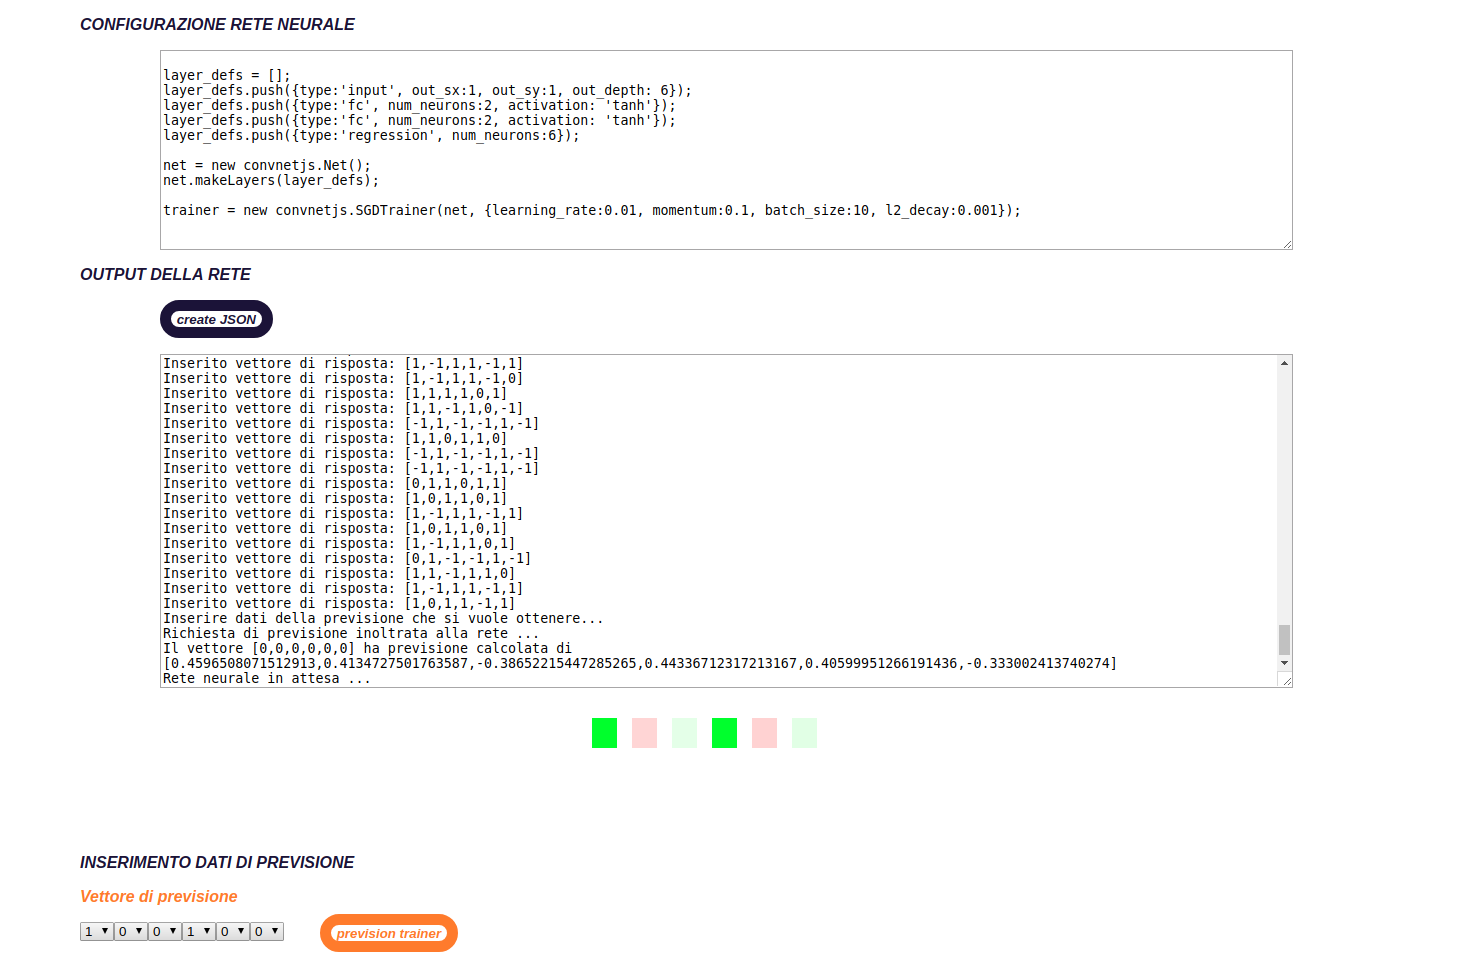
\includegraphics[width=0.90\linewidth]{./image/rete_prova-canvas.png}
	\caption{Rete di prova dopo lo sviluppo del canvas per le previsioni.}
\end{figure}

\begin{figure}[H]
\centering
	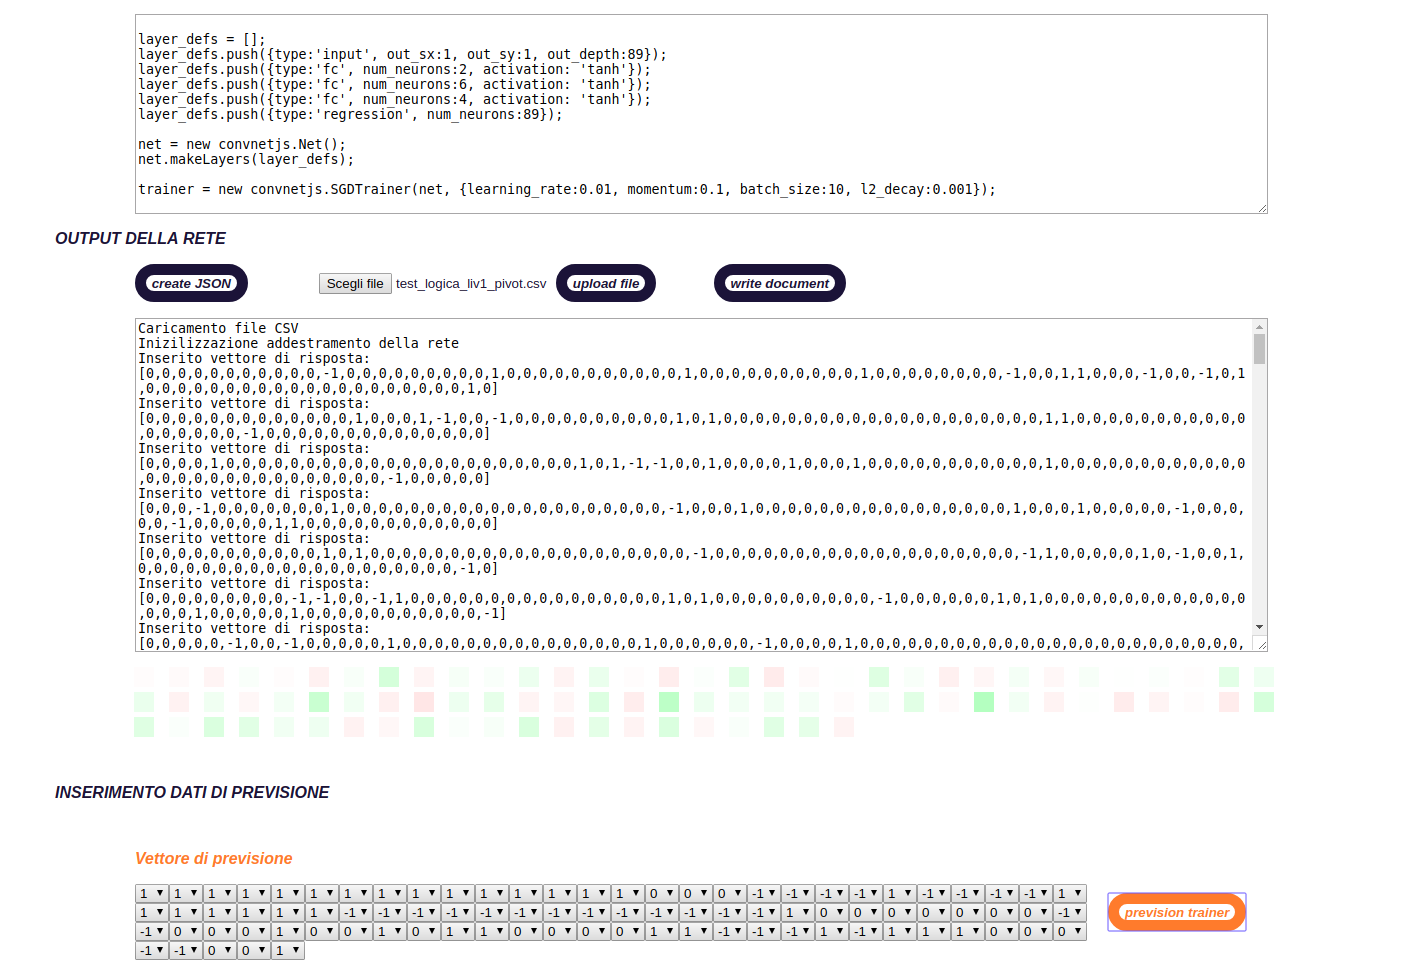
\includegraphics[width=0.90\linewidth]{./image/rete_db.png}
	\caption{Rete neurale del database aziendale.}
\end{figure}
 
L'architettura che ho utilizzato, basandomi anche sul quanto appreso dalla rete neurale di prova e dal numero di vettori di test utilizzati (1245 vettori x 89) ho aumentato le dimensioni della rete.
\begin{verbatim}
layer_defs = [];
layer_defs.push({type:'input', out_sx:1, out_sy:1, out_depth:89});
layer_defs.push({type:'fc', num_neurons:2, activation: 'tanh'});
layer_defs.push({type:'fc', num_neurons:6, activation: 'tanh'});
layer_defs.push({type:'fc', num_neurons:4, activation: 'tanh'});
layer_defs.push({type:'regression', num_neurons:89});

net = new convnetjs.Net();
net.makeLayers(layer_defs);

trainer = new convnetjs.SGDTrainer(net, {learning_rate:0.01,
momentum:0.1, batch_size:10, l2_decay:0.001});
\end{verbatim}
Ho aggiunto un layer e messo un numero di neuroni per layer in modo da formare un romboide. Devo verificare la bont\`a di questa mia scelta o se invece mi porta ad una situazione di overfitting.


Analizzando il training set dei vettori ho riscontrato tali correlazioni:
\begin{itemize}
\item Solo una piccola parte delle domande presenti in un database vengono svolte durante un colloquio con un candidato, in media una decina su 89 possibili;
\item Dalla rete sembra che le domande abbiano qualche correlazione, tuttavia la configurazione attuale ne rende difficoltosa l'individuazione.
\end{itemize}

\subsubsection{Test e Documentazione}
\label{Test e Documentazione}
Durante la settimana dal 10/06 al 18/06 ho effettuato quanto definito come "Test e Documentazione".
e definito una configurazione delle previsioni al dettaglio che permette di individuare con maggiore facilit\`a quelle che sono le relazioni esistenti tra le domande dei test.

\paragraph{Test nella Rete di prova}\mbox{}\\\\
\label{Test nella Rete di prova}
\noindent

\begin{itemize}
\item \begin{verbatim}Il vettore [1,1,1,1,1,1] ha previsione calcolata di
[0.8521066399598267,0.898137375081856,0.9993098151218291,0.792190337086403,
0.811145866789799,0.9514731560722426]
\end{verbatim}

\begin{figure}[H]
\centering
	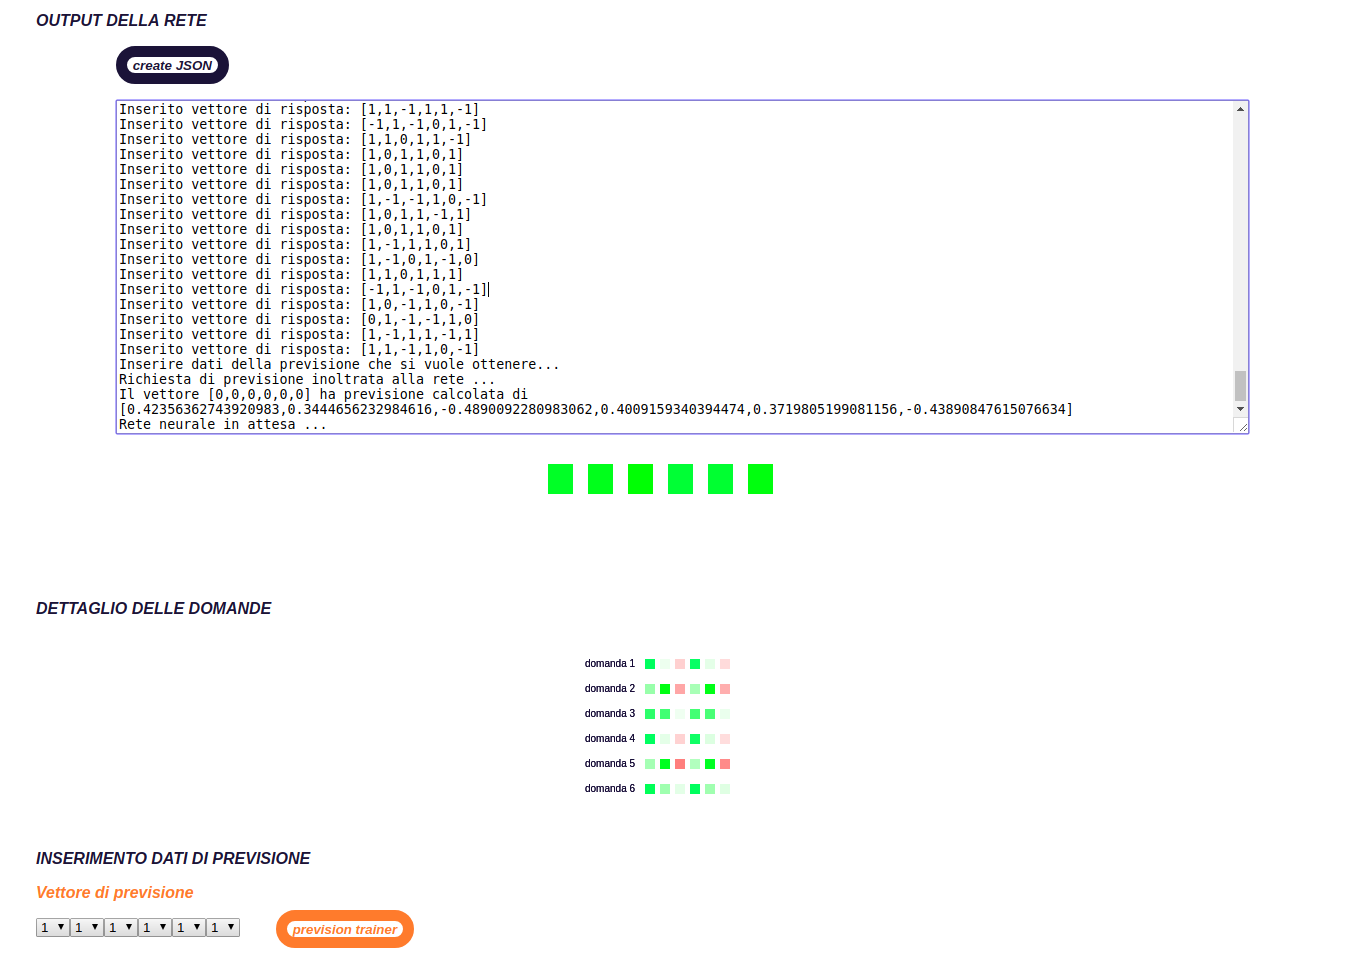
\includegraphics[width=0.90\linewidth]{./image/rete_prova-vp1.png}
	\caption{Risultato della rete di prova a seguito di un vettore di previsione [1, 1, 1, 1, 1, 1] in input.}
\end{figure}
Quanto mostrato dal dettaglio delle domande ha il seguente significato per un candidato:
\begin{itemize}
\item \textit{se la domanda 1 \`e settata a 1 (corretta)}: la rete prevede che la domanda 1 e 4 abbiano una probabilit\`a alta di essere risposte in modo corretto (verde); la 3 e 6 una probabilit\`a non eccessiva di venire risposte in modo sbagliato (rosa attenuato), la 2 e la 5 di non venire nemmeno poste (bianco con qualche minima sfumatura di verde).
\item \textit{se la domanda 2 \`e settata a 1 (corretta)}: la rete prevede che la domanda 1 e 4 abbiano una probabilit\`a non molto alta di essere risposte in modo corretto (bianco con qualche sfumatura di verde); la 3 e 6 una buona probabilit\`a di venire risposte in modo sbagliato (rosa), la 2 e la 5 di venire date in modo corretto (verde).
\item \textit{se la domanda 3 \`e settata a 1 (corretta)}: la rete prevede che la domanda 3 e 6 abbiano una probabilit\`a comunque bassa di essere risposte in modo corretto (bianco con qualche sfumatura di verde); la 1 e 4 con probabilit\`a di venire risposte in modo corretto (verde) perch\`e pi\`u semplici delle domande 3 e 6, la 2 e la 5 di venire risposte correttamente (verde).
\item \textit{se la domanda 4 \`e settata a 1 (corretta)}: la rete prevede un risultato  identico a quanto ottenuto dalla domanda 1.
\item \textit{se la domanda 5 \`e settata a 1 (corretta)}: la rete prevede un risultato similare a quanto ottenuto dalla domanda 2. Cambia solo quanto previsto dalle domande 3 e 6 che si presentano con un rosa un p\`o pi\`u intenso, in quanto con correlate alla coppia di domande 2 e 5.
\item \textit{se la domanda 6 \`e settata a 1 (corretta)}: la rete prevede un risultato simile a quanto ottenuto dalla domanda 3. La coppia 2 e 5 hanno una probabilit\`a minore di essere date correttamente (bianco con sfumature di verde) ma perch\`e non correlate alle domande 3 e 6.
\end{itemize}

\item \begin{verbatim}Il vettore [-1,-1,-1,-1,-1,-1] ha previsione calcolata di
[0.3440856175367477,-0.5026946644729329,-1.284368009920025,
0.35883842020377565,-0.37844446052773495,-1.1717763012412878]
\end{verbatim}

\begin{figure}[H]
\centering
	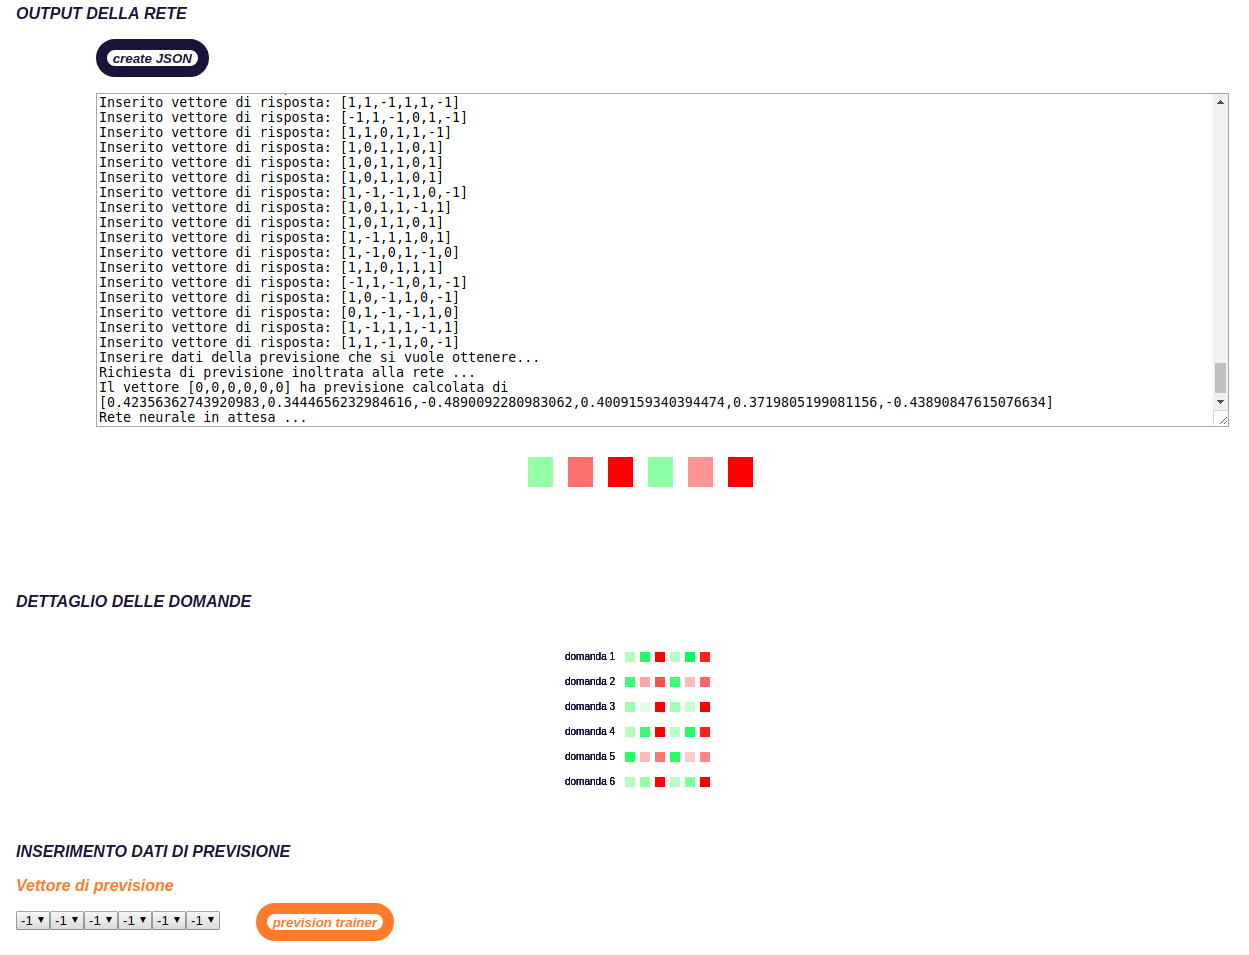
\includegraphics[width=0.90\linewidth]{./image/rete_prova-vpmeno1.png}
	\caption{Risultato della rete di prova a seguito di un vettore di previsione [-1, -1, -1, -1, -1, -1] in input.}
\end{figure}
\begin{itemize}
\item \textit{se la domanda 1 \`e settata a -1 (non corretta)}: la rete prevede che la domanda 1 e 4 non abbiano una probabilit\`a alta di essere risposte in modo corretto (bianco con sfumature di verde); la 3 e 6 una probabilit\`a molto alta di venire risposte in modo sbagliato (rosso), la 2 e la 5 di non venire nemmeno poste (verde con qualche sfumatura di bianco).
\item \textit{se la domanda 2 \`e settata a -1 (non corretta)}: la rete prevede che la domanda 1 e 4 abbiano una probabilit\`a non molto alta di essere risposte in modo non corretto (verde con qualche sfumatura di bianco); la 3 e 6 una buona probabilit\`a di venire risposte in modo sbagliato (rosa), la 2 e la 5 di venire date in modo non corretto (rosa molto atenuato).
\item \textit{se la domanda 3 \`e settata a -1 (non corretta)}: la rete prevede che la domanda 3 e 6 abbiano una probabilit\`a comunque alta di essere risposte in modo non corretto (rosso); la 1 e 4 con bassa probabilit\`a di venire risposte in modo corretto (bianco con qualche sfumatura di verde) perch\`e pi\`u semplici delle domande 3 e 6, la 2 e la 5 di non venire nemmeno poste o comunque basso di venire risposto correttamente(bianco con sfumature di verde).
\item \textit{se la domanda 4 \`e settata a -1 (non corretta)}: la rete prevede un risultato  identico a quanto ottenuto dalla domanda 1.
\item \textit{se la domanda 5 \`e settata a -1 (non corretta)}: la rete prevede un risultato similare a quanto ottenuto dalla domanda 2. Cambia solo quanto previsto dalle domande 3 e 6 che si presentano con un rosa un p\`o meno intenso, in quanto non  correlate alla coppia di domande 2 e 5.
\item \textit{se la domanda 6 \`e settata a -1 (non corretta)}: la rete prevede un risultato simile a quanto ottenuto dalla domanda 3. La coppia 2 e 5 hanno una probabilit\`a maggiore di essere date correttamente (bianco con sfumature di verde) ma perch\`e non correlate alle domande 3 e 6.
\end{itemize}
\end{itemize}

\paragraph{Test nella Rete del database}\mbox{}\\\\
\label{Test nella Rete del database}
\noindent

\begin{figure}[H]
\centering
	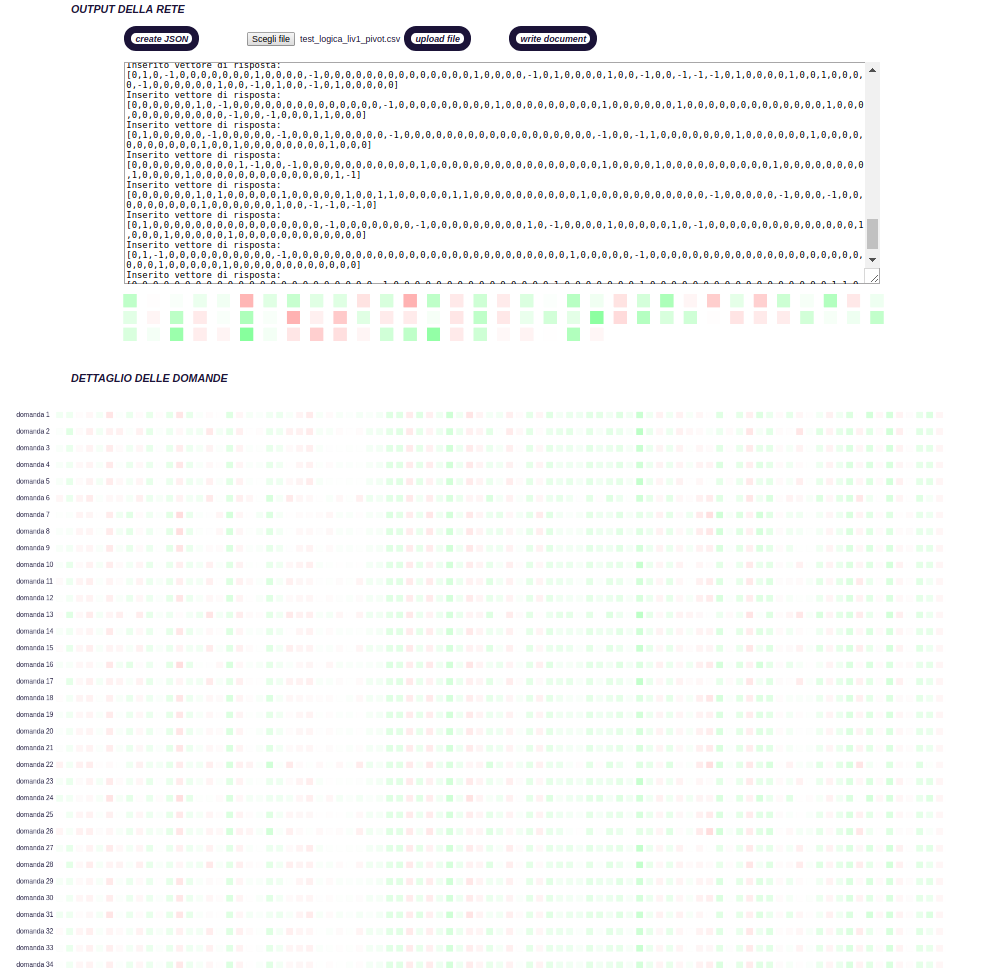
\includegraphics[width=0.90\linewidth]{./image/rete_db-vp1.png}
	\caption{Risultato della rete del database a seguito di un vettore di previsione [1, 1, 1, 1, 1, 1] in input.}
\end{figure}

\begin{figure}[H]
\centering
	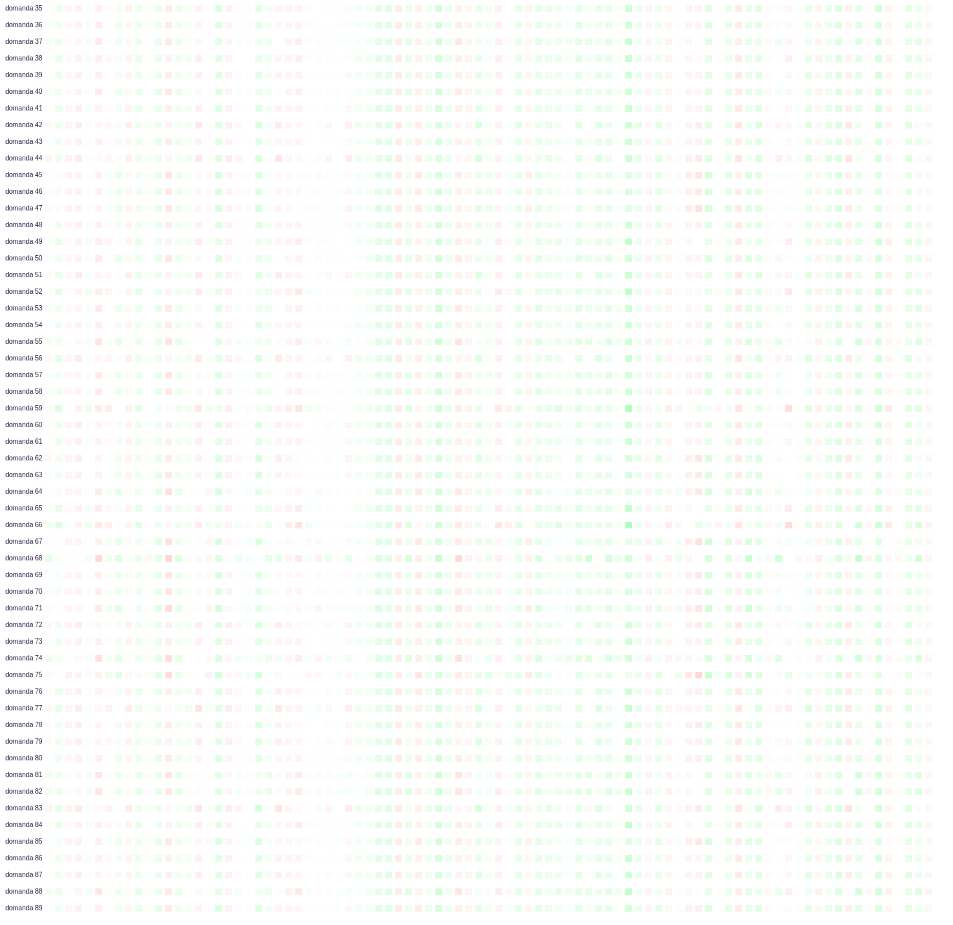
\includegraphics[width=0.90\linewidth]{./image/rete_db-vp1_2.png}
	\caption{Risultato della rete del database a seguito di un vettore di previsione [1, 1, 1, 1, 1, 1] in input.}
\end{figure}

Dagli screen della rete riportati sopra appare come "sembrano" domande:
\begin{enumerate}
\item Analisi verticale:
\begin{itemize}
\item \textit{semplici} la 18, 22, 34, 35, 37, 39, 41, 44, 48, 50, 51, 52, 53, 54, 55, 56, 57, 59, 60, 67, 69,  71, 72, 77, 79, 80, 82, 84, 87 e 88. Inoltre di queste sembrano in relazione ancora pi\`u stretta le domande 18, 22, 40 e 59.
\item \textit{difficili} la 3, 4, 6, 13, 16, 19, 24, 25, 26, 36, 38, 42, 43, 46, 49, 61, 63, 65, 66, 70, 78, 81, 85 e 89. Inoltre di queste sembrano in relazione ancora pi\`u stretta le domande 6, 13, 19, 36, 38, 42, 46 e 70.
\end{itemize}
\item Analisi orizzontale:
Appaiono in relazione stretta le seguenti domande:
\begin{itemize}
\item 2, 3, 4, 5;
\item 7, 8, 9;
\item 14, 16;
\item 20, 21;
\item 26, 32;
\item 29, 32
\item 33, 34, 35, 36, 38;
\item 39, 41, 43;
\item 46, 48;
\item 49, 52;
\item 50, 53;
\item 72, 79;
\item 81, 82;
\item 86, 87, 88.
\end{itemize}
\end{enumerate}

\begin{figure}[H]
\centering
	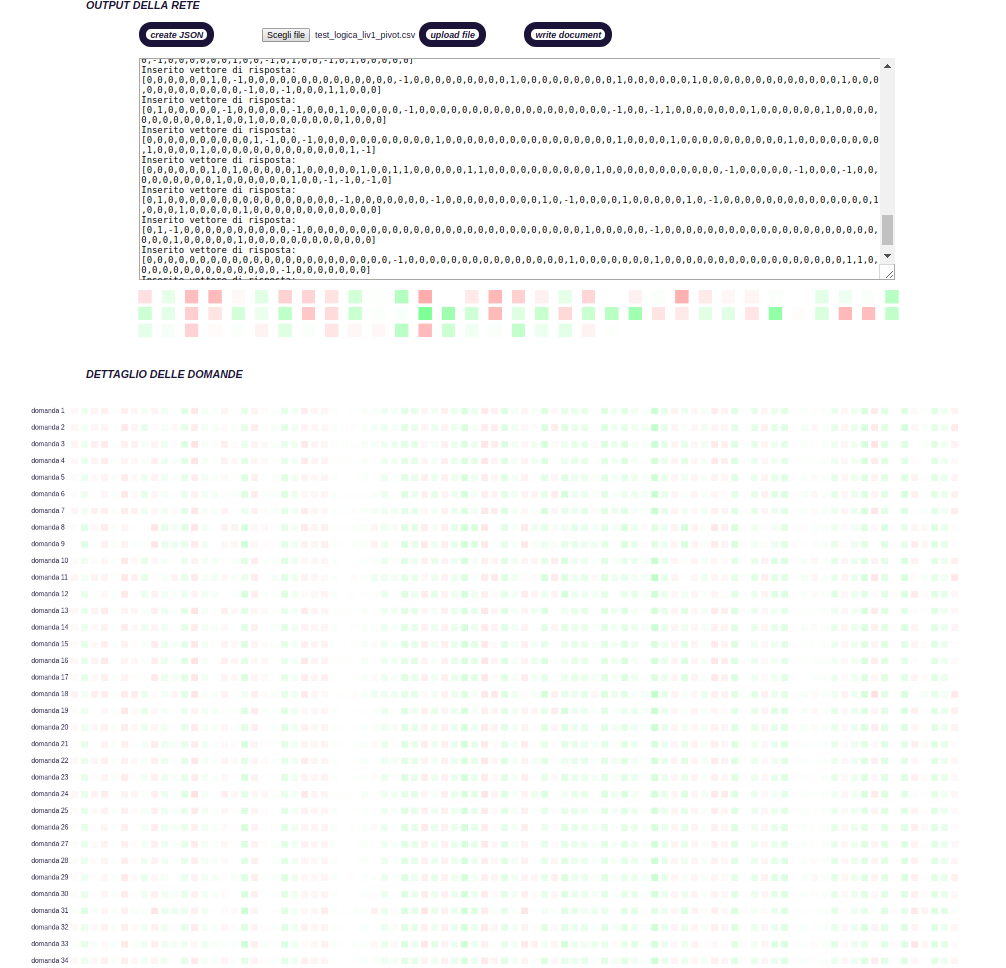
\includegraphics[width=0.90\linewidth]{./image/rete_db-vpmeno1.png}
	\caption{Risultato della rete del database a seguito di un vettore di previsione [-1, -1, -1, -1, -1, -1] in input.}
\end{figure}

\begin{figure}[H]
\centering
	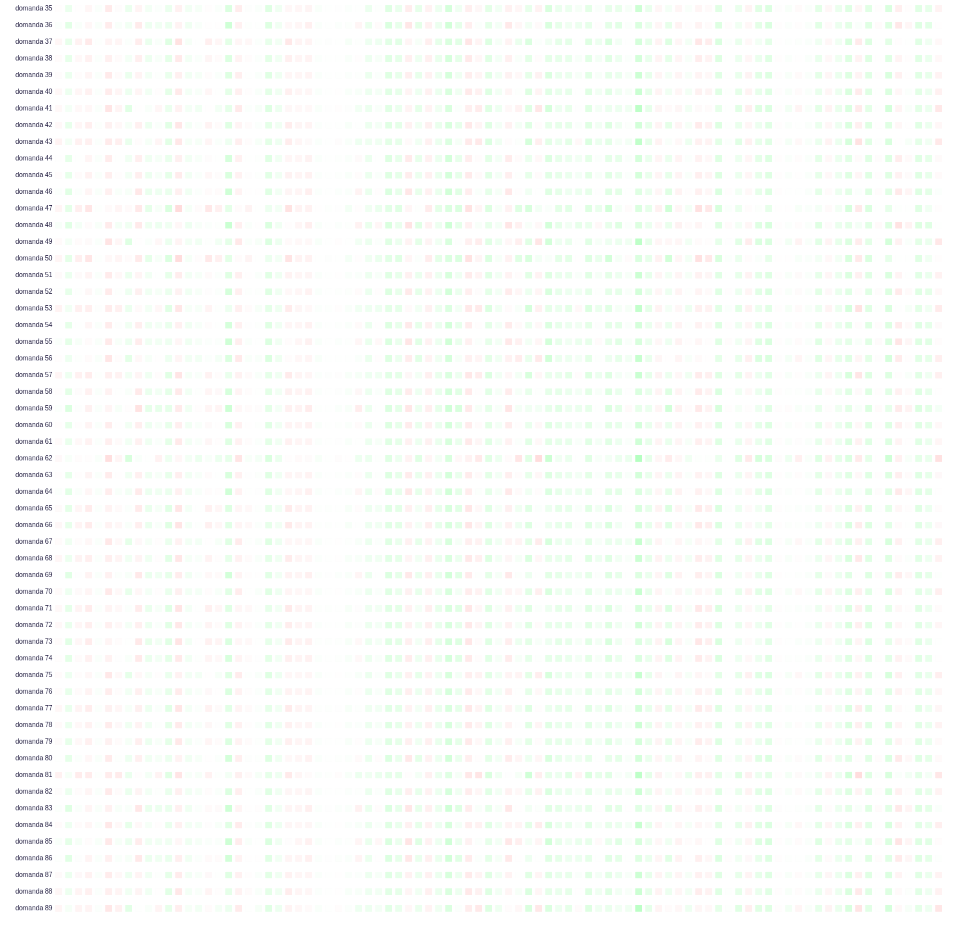
\includegraphics[width=0.90\linewidth]{./image/rete_db-vpmeno1_2.png}
	\caption{Risultato della rete del database a seguito di un vettore di previsione [-1, -1, -1, -1, -1, -1] in input.}
\end{figure}

Dagli screen della rete riportati sopra appare come "sembrano" domande:
\begin{enumerate}
\item Analisi verticale:
\begin{itemize}
\item \textit{semplici} la 18, 22, 34, 35, 37, 38, 39, 41, 44, 48, 50, 51, 52, 54, 55, 56, 67, 69,  71, 72, 77, 79, 80, 82, 84, 87 e 88. Inoltre di queste sembrano in relazione ancora pi\`u stretta le domande 18, 22, 38, 52 e 57.
\item \textit{difficili} la 3, 4, 6, 13, 19, 27, 36, 38, 42, 43, 46, 61, 62, 65, 70. Inoltre di queste sembrano in relazione ancora pi\`u stretta le domande 6, 13, 19, 36, 38, 42, 46, 61 e 62.
\end{itemize}
\item Analisi orizzontale:
Appaiono in relazione stretta le seguenti domande:
\begin{itemize}
\item rimaste consistenti con il vettore [1, 1, 1, 1, 1, 1].
\end{itemize}
\end{enumerate}


\subparagraph{Previsioni di diverse architetture di rete}
\label{Previsioni di diverse architetture di rete}
\begin{verbatim}
layer_defs = [];
layer_defs.push({type:'input', out_sx:1, out_sy:1, out_depth:89});
layer_defs.push({type:'fc', num_neurons:12, activation: 'tanh'});
layer_defs.push({type:'regression', num_neurons:89});

net = new convnetjs.Net();
net.makeLayers(layer_defs);

trainer = new convnetjs.SGDTrainer(net, {learning_rate:0.01, momentum:0.1, batch_size:10, l2_decay:0.001});
\end{verbatim}
La prima cosa che ho notato \`e che aumentando il numero di neuroni sull'unico layer esistente, il valore della domanda corrispondente al vettore della previsione sembra sempre pi\`u marcato, segno che la rete "impara troppo" e ricade nel restituire l'immagine stessa del vettore previsione.

\begin{figure}[H]
\centering
	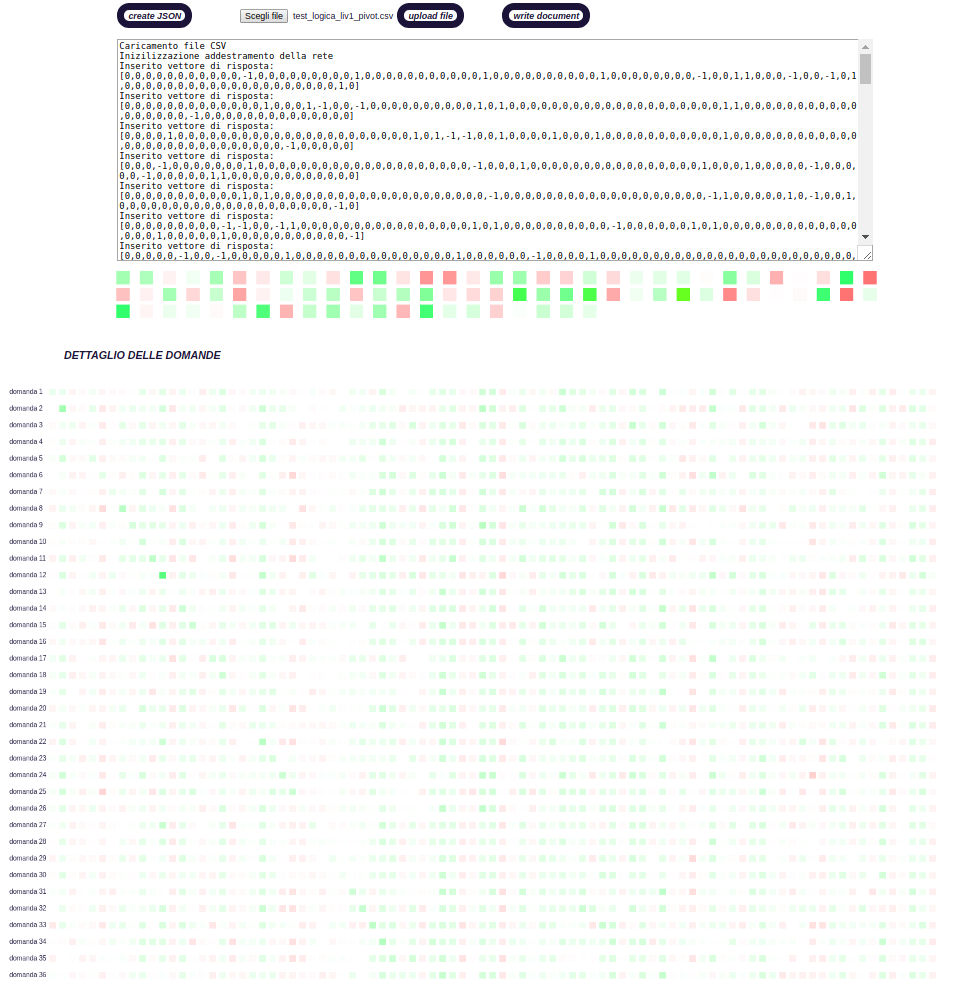
\includegraphics[width=0.90\linewidth]{./image/rete_db-vp1architettura2.png}
	\caption{Risultato della rete del database a seguito di un vettore di previsione [1, 1, 1, 1, 1, 1] in input.}
\end{figure}

\begin{figure}[H]
\centering
	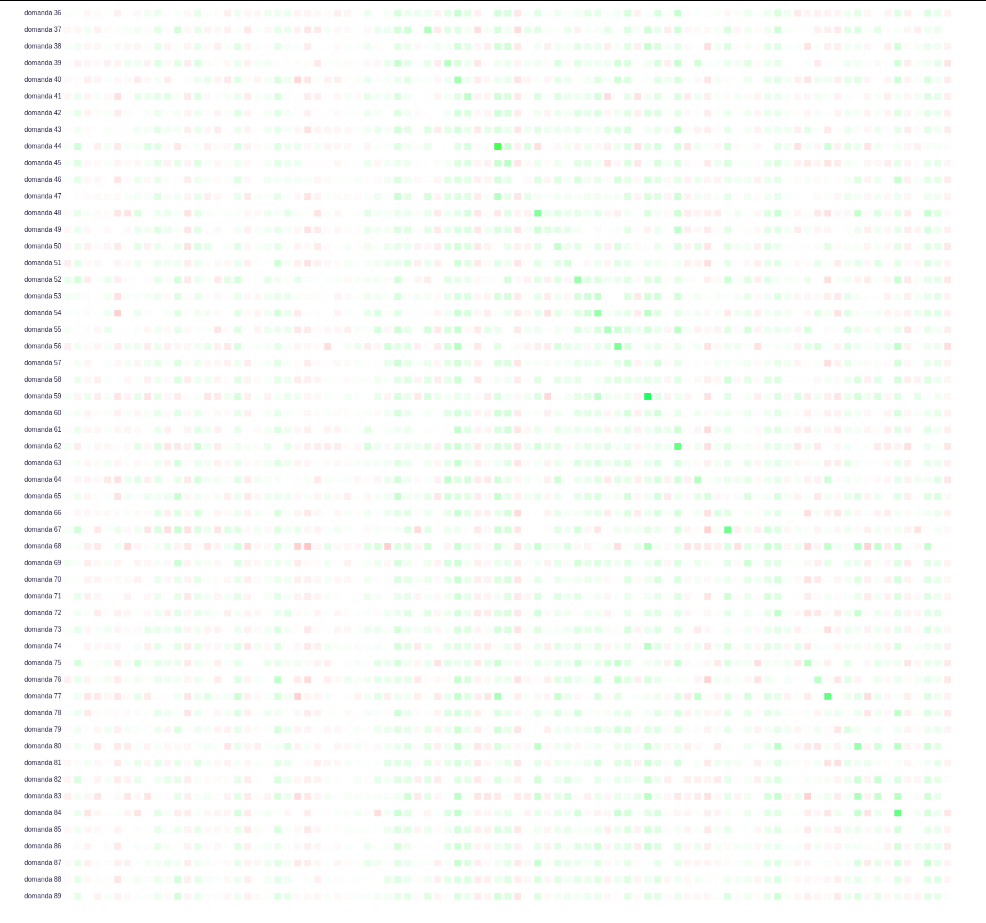
\includegraphics[width=0.90\linewidth]{./image/rete_db-vp1_2architettura2.png}
	\caption{Risultato della rete del database a seguito di un vettore di previsione [1, 1, 1, 1, 1, 1] in input.}
\end{figure}

Dagli screen della rete riportati sopra appare come la situazione appare meno lineare del caso analizzato precedentemente. 
Le domande non vengono separate per linee rete; ma per aree di relazione.


Dagli screen della rete riportati sopra appare come "sembrano" domande:
\begin{enumerate}
\item Analisi verticale:
\begin{itemize}
\item \textit{semplici} la 18, 22, 34, 35, 37, 39, 41, 44, 48, 50, 51, 52, 53, 54, 55, 56, 57, 59, 60, 67, 69,  71, 72, 77, 79, 80, 82, 84, 87 e 88. Inoltre di queste sembrano in relazione ancora pi\`u stretta le domande 18, 22, 40 e 59.
\item \textit{difficili} la 3, 4, 6, 13, 16, 19, 24, 25, 26, 36, 38, 42, 43, 46, 49, 61, 63, 65, 66, 70, 78, 81, 85 e 89. Inoltre di queste sembrano in relazione ancora pi\`u stretta le domande 6, 13, 19, 36, 38, 42, 46 e 70.
\end{itemize}
\item Analisi orizzontale:
Appaiono in relazione stretta le seguenti domande:
\begin{itemize}
\item Vengono meno le relazioni individuate precedentemente.
\end{itemize}
\end{enumerate}

Test archittettura 

layer_defs = [];
layer_defs.push({type:'input', out_sx:1, out_sy:1, out_depth:89});
layer_defs.push({type:'fc', num_neurons:2, activation: 'tanh'});
layer_defs.push({type:'fc', num_neurons:6, activation: 'tanh'});
layer_defs.push({type:'fc', num_neurons:4, activation: 'tanh'});
layer_defs.push({type:'regression', num_neurons:89});

net = new convnetjs.Net();
net.makeLayers(layer_defs);

trainer = new convnetjs.SGDTrainer(net, {learning_rate:0.01, momentum:0.1, batch_size:10, l2_decay:0.001});

- differenza tra i valori nei vettori di < 1: non ottengo alcuna correlazione tra le domande tranne loro stesse
- differenza di <= 1

* vettore previsione a 1
Rete neurale in attesa ...
Relazione fra le domande :
domanda 1:[1]
domanda 2:[2,27]
domanda 3:[3,89]
domanda 4:[4,83]
domanda 5:[5]
domanda 6:[6,62]
domanda 7:[7,42]
domanda 8:[8,71]
domanda 9:[9]
domanda 10:[10,18]
domanda 11:[11]
domanda 12:[12,28,58]
domanda 13:[13]
domanda 14:[14,53,66,72]
domanda 15:[15,30]
domanda 16:[16,67]
domanda 17:[17]
domanda 18:[10,18]
domanda 19:[19,20]
domanda 20:[19,20]
domanda 21:[21]
domanda 22:[22]
domanda 23:[23,55]
domanda 24:[24]
domanda 25:[25,62,76]
domanda 26:[26]
domanda 27:[2,27]
domanda 28:[12,28,58]
domanda 29:[29]
domanda 30:[15,30]
domanda 31:[31]
domanda 32:[32,41]
domanda 33:[33]
domanda 34:[34]
domanda 35:[35,36]
domanda 36:[35,36]
domanda 37:[37,51]
domanda 38:[38]
domanda 39:[39]
domanda 40:[40,79]
domanda 41:[32,41]
domanda 42:[7,42]
domanda 43:[43]
domanda 44:[44]
domanda 45:[45]
domanda 46:[46,48]
domanda 47:[47]
domanda 48:[46,48]
domanda 49:[49]
domanda 50:[50]
domanda 51:[37,51]
domanda 52:[52]
domanda 53:[14,53]
domanda 54:[54]
domanda 55:[23,55,56]
domanda 56:[55,56]
domanda 57:[57]
domanda 58:[12,28,58]
domanda 59:[59]
domanda 60:[60]
domanda 61:[61]
domanda 62:[6,25,62]
domanda 63:[63]
domanda 64:[64]
domanda 65:[65]
domanda 66:[14,66]
domanda 67:[16,67]
domanda 68:[68]
domanda 69:[69]
domanda 70:[70]
domanda 71:[8,71]
domanda 72:[14,72]
domanda 73:[73]
domanda 74:[74]
domanda 75:[75]
domanda 76:[25,76]
domanda 77:[77]
domanda 78:[78]
domanda 79:[40,79]
domanda 80:[80]
domanda 81:[81]
domanda 82:[82]
domanda 83:[4,83]
domanda 84:[84]
domanda 85:[85]
domanda 86:[86]
domanda 87:[87]
domanda 88:[88]
domanda 89:[3,89]

* vettore previsione a -1
Relazione fra le domande :
domanda 1:[1]
domanda 2:[2,27]
domanda 3:[3]
domanda 4:[4,83]
domanda 5:[5]
domanda 6:[6,62]
domanda 7:[7,42]
domanda 8:[8,71]
domanda 9:[9]
domanda 10:[10]
domanda 11:[11]
domanda 12:[12]
domanda 13:[13]
domanda 14:[14,53,66]
domanda 15:[15,30,78,86]
domanda 16:[16,67]
domanda 17:[17]
domanda 18:[18]
domanda 19:[19,20]
domanda 20:[19,20]
domanda 21:[21]
domanda 22:[22]
domanda 23:[23,55,56]
domanda 24:[24]
domanda 25:[25,62,76]
domanda 26:[26]
domanda 27:[2,27]
domanda 28:[28,58]
domanda 29:[29]
domanda 30:[15,30,78,86]
domanda 31:[31]
domanda 32:[32,41]
domanda 33:[33]
domanda 34:[34]
domanda 35:[35,36]
domanda 36:[35,36]
domanda 37:[37,51]
domanda 38:[38]
domanda 39:[39]
domanda 40:[40,79]
domanda 41:[32,41]
domanda 42:[7,42]
domanda 43:[43]
domanda 44:[44]
domanda 45:[45]
domanda 46:[46]
domanda 47:[47]
domanda 48:[48]
domanda 49:[49]
domanda 50:[50]
domanda 51:[37,51]
domanda 52:[52]
domanda 53:[14,53]
domanda 54:[54]
domanda 55:[23,55,56]
domanda 56:[23,55,56]
domanda 57:[57]
domanda 58:[28,58]
domanda 59:[59]
domanda 60:[60]
domanda 61:[61]
domanda 62:[6,25,62]
domanda 63:[63]
domanda 64:[64]
domanda 65:[65]
domanda 66:[14,66]
domanda 67:[16,67]
domanda 68:[68]
domanda 69:[69]
domanda 70:[70]
domanda 71:[8,71]
domanda 72:[72]
domanda 73:[73]
domanda 74:[74]
domanda 75:[75]
domanda 76:[25,76]
domanda 77:[77]
domanda 78:[15,30,78]
domanda 79:[40,79]
domanda 80:[80]
domanda 81:[81]
domanda 82:[82]
domanda 83:[4,83]
domanda 84:[84]
domanda 85:[85]
domanda 86:[15,30,86]
domanda 87:[87]
domanda 88:[88]
domanda 89:[89]

- differenza di <= 2

* Vettore previsione a 1
Relazione fra le domande :
domanda 1:[1]
domanda 2:[2,79]
domanda 3:[3,22,71,73]
domanda 4:[4,35,55,89]
domanda 5:[5,28,56,57,83]
domanda 6:[6,12,19,43,52]
domanda 7:[7,49,50,82]
domanda 8:[8,29,39,65,87]
domanda 9:[9,78]
domanda 10:[10,36,40]
domanda 11:[11,13]
domanda 12:[6,12,19,43,52]
domanda 13:[11,13,35]
domanda 14:[14,51]
domanda 15:[15,75]
domanda 16:[16]
domanda 17:[17,18,36,40,59]
domanda 18:[17,18,36,59]
domanda 19:[6,12,19,31,43]
domanda 20:[20,39,46,88]
domanda 21:[21,23,28,69]
domanda 22:[3,22,85]
domanda 23:[21,23]
domanda 24:[24,26]
domanda 25:[25]
domanda 26:[24,26,61]
domanda 27:[27,41,45,60]
domanda 28:[5,21,28,56,57]
domanda 29:[8,29,65,87]
domanda 30:[30,40,42,88]
domanda 31:[19,31]
domanda 32:[32,33,48,73,74]
domanda 33:[32,33,48,74]
domanda 34:[34]
domanda 35:[4,13,35]
domanda 36:[10,17,18,36,40,59]
domanda 37:[37]
domanda 38:[38,49,67]
domanda 39:[8,20,39,46]
domanda 40:[10,17,30,36,40]
domanda 41:[27,41,45]
domanda 42:[30,42,88]
domanda 43:[6,12,19,43]
domanda 44:[44]
domanda 45:[27,41,45,60]
domanda 46:[20,39,46]
domanda 47:[47]
domanda 48:[32,33,48]
domanda 49:[7,38,49,50,67]
domanda 50:[7,49,50,82]
domanda 51:[14,51]
domanda 52:[6,12,52]
domanda 53:[53]
domanda 54:[54]
domanda 55:[4,55,89]
domanda 56:[5,28,56,57]
domanda 57:[5,28,56,57,72,83]
domanda 58:[58,66,70]
domanda 59:[17,18,36,59]
domanda 60:[27,45,60]
domanda 61:[26,61]
domanda 62:[62]
domanda 63:[63,76]
domanda 64:[64]
domanda 65:[8,29,65,68,87]
domanda 66:[58,66,70]
domanda 67:[38,49,67]
domanda 68:[65,68,87]
domanda 69:[21,69]
domanda 70:[58,66,70]
domanda 71:[3,71]
domanda 72:[57,72,85]
domanda 73:[3,32,73]
domanda 74:[32,33,74]
domanda 75:[15,75]
domanda 76:[63,76]
domanda 77:[77]
domanda 78:[9,78]
domanda 79:[2,79]
domanda 80:[80]
domanda 81:[81]
domanda 82:[7,50,82]
domanda 83:[5,57,83]
domanda 84:[84]
domanda 85:[22,72,85]
domanda 86:[86]
domanda 87:[8,29,65,68,87]
domanda 88:[20,30,42,88]
domanda 89:[4,55,89]


* Vettore previsione a -1
Relazione fra le domande :
domanda 1:[1]
domanda 2:[2,79]
domanda 3:[3,22,71]
domanda 4:[4,35,55,89]
domanda 5:[5,28,56,57,83]
domanda 6:[6,12,19,43,52]
domanda 7:[7,49,50,67,82]
domanda 8:[8,29,65,87]
domanda 9:[9,78]
domanda 10:[10,36]
domanda 11:[11,13]
domanda 12:[6,12,19,31,43,52]
domanda 13:[11,13]
domanda 14:[14,51]
domanda 15:[15,47,75]
domanda 16:[16,38]
domanda 17:[17,18,36,40,59]
domanda 18:[17,18,36,59]
domanda 19:[6,12,19,31,43]
domanda 20:[20,46,88]
domanda 21:[21,28,69]
domanda 22:[3,22,85]
domanda 23:[23,60]
domanda 24:[24,26]
domanda 25:[25]
domanda 26:[24,26,61]
domanda 27:[27,45,60]
domanda 28:[5,21,28,56,57]
domanda 29:[8,29,65]
domanda 30:[30,42,88]
domanda 31:[12,19,31]
domanda 32:[32,33,73,74]
domanda 33:[32,33,48,74]
domanda 34:[34]
domanda 35:[4,35]
domanda 36:[10,17,18,36,40,59]
domanda 37:[37]
domanda 38:[16,38,49]
domanda 39:[39,46,68]
domanda 40:[17,36,40]
domanda 41:[41]
domanda 42:[30,42,88]
domanda 43:[6,12,19,43]
domanda 44:[44]
domanda 45:[27,45,60]
domanda 46:[20,39,46]
domanda 47:[15,47]
domanda 48:[33,48,74]
domanda 49:[7,38,49,50,67]
domanda 50:[7,49,50,82]
domanda 51:[14,51]
domanda 52:[6,12,52]
domanda 53:[53,62]
domanda 54:[54]
domanda 55:[4,55,89]
domanda 56:[5,28,56,57,72]
domanda 57:[5,28,56,57,72]
domanda 58:[58,66,70]
domanda 59:[17,18,36,59]
domanda 60:[23,27,45,60]
domanda 61:[26,61]
domanda 62:[53,62]
domanda 63:[63,76]
domanda 64:[64]
domanda 65:[8,29,65,87]
domanda 66:[58,66,70]
domanda 67:[7,49,67]
domanda 68:[39,68,87]
domanda 69:[21,69]
domanda 70:[58,66,70]
domanda 71:[3,71]
domanda 72:[56,57,72,85]
domanda 73:[32,73]
domanda 74:[32,33,48,74]
domanda 75:[15,75]
domanda 76:[63,76]
domanda 77:[77]
domanda 78:[9,78]
domanda 79:[2,79]
domanda 80:[80]
domanda 81:[81]
domanda 82:[7,50,82]
domanda 83:[5,83]
domanda 84:[84]
domanda 85:[22,72,85]
domanda 86:[86]
domanda 87:[8,65,68,87]
domanda 88:[20,30,42,88]
domanda 89:[4,55,89]

- differenza <= 5
* Vettore di previsione a -1
Relazione fra le domande :
domanda 1:[1,6,11,52,68,71,74,84,85]
domanda 2:[2]
domanda 3:[3,10,16,17,19,26,32,33,35,41,42,46,51,57,58,60,63,70,86,89]
domanda 4:[4,5,12,15,20,21,23,26,28,30,32,33,38,51,53,58,62,73,79,81]
domanda 5:[4,5,20,21,22,28,31,40,48,64,79,81]
domanda 6:[1,6,12,16,17,23,25,38,52,58,60,70,71,74,84,85]
domanda 7:[7,13,14,29,50,66,78,88]
domanda 8:[8,18,22,75,83]
domanda 9:[9]
domanda 10:[3,10,15,17,19,21,28,29,32,33,35,41,42,57,62,63,66,78,79,86,89]
domanda 11:[1,11,43,52,56,68,71,76,85]
domanda 12:[4,6,12,15,20,23,25,26,28,30,32,33,38,39,41,42,51,53,58,60,62,63,70,73,84]
domanda 13:[7,13,14,29,31,40,49,50,64,88]
domanda 14:[7,13,14,29,31,40,48,49,50,64,79,81,88]
domanda 15:[4,10,12,15,17,19,20,21,26,28,30,32,33,35,41,42,51,58,62,63,66,73,79,81,89]
domanda 16:[3,6,16,17,26,32,41,42,46,58,60,63,70,74,86]
domanda 17:[3,6,10,15,16,17,19,23,25,26,32,33,35,38,41,42,46,51,58,60,62,63,70,84,86,89]
domanda 18:[8,18,75]
domanda 19:[3,10,15,17,19,21,26,28,32,33,35,41,42,46,51,57,58,60,62,63,66,70,78,79,86,89]
domanda 20:[4,5,12,15,20,21,23,28,30,38,51,53,62,73,79,81]
domanda 21:[4,5,10,15,19,20,21,28,30,31,32,33,35,40,41,48,51,62,63,66,73,79,81,89]
domanda 22:[5,8,22,75,83]
domanda 23:[4,6,12,17,20,23,25,26,30,32,33,38,39,41,42,51,53,58,60,62,63,70,73,84]
domanda 24:[24,69]
domanda 25:[6,12,17,23,25,26,30,32,33,38,39,41,42,51,53,58,60,62,63,70,73,84]
domanda 26:[3,4,12,15,16,17,19,23,25,26,28,30,32,33,35,38,41,42,46,51,58,60,62,63,70,73,84,86,89]
domanda 27:[27,61,80,83,87]
domanda 28:[4,5,10,12,15,19,20,21,26,28,30,31,32,33,35,40,41,42,48,51,62,63,66,73,79,81,89]
domanda 29:[7,10,13,14,29,40,49,50,66,78,79,88]
domanda 30:[4,12,15,20,21,23,25,26,28,30,32,38,39,51,53,58,62,73,79,84]
domanda 31:[5,13,14,21,28,31,40,48,49,64,79,81]
domanda 32:[3,4,10,12,15,16,17,19,21,23,25,26,28,30,32,33,35,38,41,42,46,51,58,60,62,63,66,70,73,84,86,89]
domanda 33:[3,4,10,12,15,17,19,21,23,25,26,28,32,33,35,38,41,42,46,51,58,60,62,63,66,70,79,86,89]
domanda 34:[34,69,76]
domanda 35:[3,10,15,17,19,21,26,28,32,33,35,41,42,46,51,58,60,62,63,66,70,78,79,86,89]
domanda 36:[36,47,55,65,72,77]
domanda 37:[37,55,56,68]
domanda 38:[4,6,12,17,20,23,25,26,30,32,33,38,39,41,42,51,53,58,60,62,63,70,73,84]
domanda 39:[12,23,25,30,38,39,53,65,73,84]
domanda 40:[5,13,14,21,28,29,31,40,48,49,50,64,66,79,81,88]
domanda 41:[3,10,12,15,16,17,19,21,23,25,26,28,32,33,35,38,41,42,46,51,58,60,62,63,66,70,84,86,89]
domanda 42:[3,10,12,15,16,17,19,23,25,26,28,32,33,35,38,41,42,46,51,58,60,62,63,70,84,86,89]
domanda 43:[11,43,52,56,68,71,85]
domanda 44:[44,57,59,78]
domanda 45:[45]
domanda 46:[3,16,17,19,26,32,33,35,41,42,46,57,58,60,63,70,74,86]
domanda 47:[36,47,55,56,65,68,72,77]
domanda 48:[5,14,21,28,31,40,48,64,79,81]
domanda 49:[13,14,29,31,40,49,50,64,81,88]
domanda 50:[7,13,14,29,40,49,50,78,88]
domanda 51:[3,4,12,15,17,19,20,21,23,25,26,28,30,32,33,35,38,41,42,51,53,58,60,62,63,66,70,73,84,89]
domanda 52:[1,6,11,43,52,56,68,71,85]
domanda 53:[4,12,20,23,25,30,38,39,51,53,73,84]
domanda 54:[54,69]
domanda 55:[36,37,47,55,56,65,72,77]
domanda 56:[11,37,43,47,52,55,56,65,68,71]
domanda 57:[3,10,19,44,46,57,59,86,89]
domanda 58:[3,4,6,12,15,16,17,19,23,25,26,30,32,33,35,38,41,42,46,51,58,60,62,63,70,73,84,86,89]
domanda 59:[44,57,59,86]
domanda 60:[3,6,12,16,17,19,23,25,26,32,33,35,38,41,42,46,51,58,60,62,63,70,74,84,86]
domanda 61:[27,61,83,87]
domanda 62:[4,10,12,15,17,19,20,21,23,25,26,28,30,32,33,35,38,41,42,51,58,60,62,63,66,70,73,79,89]
domanda 63:[3,10,12,15,16,17,19,21,23,25,26,28,32,33,35,38,41,42,46,51,58,60,62,63,66,70,84,86,89]
domanda 64:[5,13,14,31,40,48,49,64,81]
domanda 65:[36,39,47,55,56,65,68,72,77]
domanda 66:[7,10,15,19,21,28,29,32,33,35,40,41,51,62,63,66,78,79,88,89]
domanda 67:[67]
domanda 68:[1,11,37,43,47,52,56,65,68,71,84,85]
domanda 69:[24,34,54,69]
domanda 70:[3,6,12,16,17,19,23,25,26,32,33,35,38,41,42,46,51,58,60,62,63,70,73,84,86]
domanda 71:[1,6,11,43,52,56,68,71,84,85]
domanda 72:[36,47,55,65,72,77,80,87]
domanda 73:[4,12,15,20,21,23,25,26,28,30,32,38,39,51,53,58,62,70,73,84]
domanda 74:[1,6,16,46,60,74,85]
domanda 75:[8,18,22,75,83]
domanda 76:[11,34,76,85]
domanda 77:[36,47,55,65,72,77,80]
domanda 78:[7,10,19,29,35,44,50,66,78,88,89]
domanda 79:[4,5,10,14,15,19,20,21,28,29,30,31,33,35,40,48,62,66,79,81,89]
domanda 80:[27,72,77,80,87]
domanda 81:[4,5,14,15,20,21,28,31,40,48,49,64,79,81]
domanda 82:[82]
domanda 83:[8,22,27,61,75,83]
domanda 84:[1,6,12,17,23,25,26,30,32,38,39,41,42,51,53,58,60,63,68,70,71,73,84]
domanda 85:[1,6,11,43,52,68,71,74,76,85]
domanda 86:[3,10,16,17,19,26,32,33,35,41,42,46,57,58,59,60,63,70,86,89]
domanda 87:[27,61,72,80,87]
domanda 88:[7,13,14,29,40,49,50,66,78,88]
domanda 89:[3,10,15,17,19,21,26,28,32,33,35,41,42,51,57,58,62,63,66,78,79,86,89]

*Vettore a -1
Relazione fra le domande :
domanda 1:[1,6,11,52,68,71,74,84,85]
domanda 2:[2]
domanda 3:[3,10,16,17,19,26,32,33,35,39,41,42,46,51,58,60,63,70,86,89]
domanda 4:[4,12,15,20,21,23,25,26,28,30,32,33,38,51,53,58,62,70,73,79,81]
domanda 5:[5,20,21,22,28,31,40,48,64,79,81]
domanda 6:[1,6,12,16,17,23,25,38,58,60,70,71,74,84,85]
domanda 7:[7,13,14,29,39,50,66,78,88]
domanda 8:[8,18,22,61,75,83]
domanda 9:[9]
domanda 10:[3,10,15,17,19,21,26,28,29,32,33,35,39,41,42,57,62,63,66,78,79,86,89]
domanda 11:[1,11,43,52,56,68,71,76,85]
domanda 12:[4,6,12,15,17,20,23,25,26,28,30,32,33,38,41,42,51,53,58,60,62,63,70,73,84]
domanda 13:[7,13,14,29,40,49,50,64,88]
domanda 14:[7,13,14,29,31,40,48,49,50,64,79,81,88]
domanda 15:[4,10,12,15,19,20,21,26,28,30,31,32,33,35,39,40,41,42,48,51,58,62,63,66,73,79,81,89]
domanda 16:[3,6,16,17,26,32,41,42,46,58,60,63,70,74,86]
domanda 17:[3,6,10,12,16,17,19,23,25,26,32,33,35,38,41,42,46,51,58,60,62,63,70,74,84,86,89]
domanda 18:[8,18,75]
domanda 19:[3,10,15,17,19,21,26,28,29,32,33,35,39,41,42,57,62,63,66,78,79,86,89]
domanda 20:[4,5,12,15,20,21,28,30,31,48,51,53,62,73,79,81]
domanda 21:[4,5,10,15,19,20,21,26,28,30,31,32,33,35,39,40,41,48,51,62,63,66,73,79,81,89]
domanda 22:[5,8,22,75,83]
domanda 23:[4,6,12,17,23,25,26,30,32,33,35,38,41,42,51,53,58,60,62,63,70,73,84]
domanda 24:[24,34,69]
domanda 25:[4,6,12,17,23,25,26,30,32,33,38,41,42,51,53,58,60,62,63,70,73,84]
domanda 26:[3,4,10,12,15,16,17,19,21,23,25,26,28,30,32,33,35,38,41,42,46,51,58,60,62,63,70,73,84,86,89]
domanda 27:[27,61,80,83,87]
domanda 28:[4,5,10,12,15,19,20,21,26,28,30,31,32,33,35,40,41,42,48,51,58,62,63,66,73,79,81,89]
domanda 29:[7,10,13,14,19,29,39,40,49,50,66,78,88,89]
domanda 30:[4,12,15,20,21,23,25,26,28,30,32,38,51,53,58,62,70,73,79]
domanda 31:[5,14,15,20,21,28,31,40,48,49,64,66,79,81]
domanda 32:[3,4,10,12,15,16,17,19,21,23,25,26,28,30,32,33,35,38,41,42,46,51,58,60,62,63,66,70,73,84,86,89]
domanda 33:[3,4,10,12,15,17,19,21,23,25,26,28,32,33,35,38,39,41,42,46,51,58,60,62,63,66,70,79,86,89]
domanda 34:[24,34,69,76]
domanda 35:[3,10,15,17,19,21,23,26,28,32,33,35,39,41,42,51,58,62,63,66,70,79,86,89]
domanda 36:[36,47,55,65,72,77]
domanda 37:[37,52,55,56,68]
domanda 38:[4,6,12,17,23,25,26,30,32,33,38,41,42,51,53,58,60,62,63,70,73,84]
domanda 39:[3,7,10,15,19,21,29,33,35,39,41,42,57,63,66,78,79,86,88,89]
domanda 40:[5,13,14,15,21,28,29,31,40,48,49,50,64,66,79,81,88]
domanda 41:[3,10,12,15,16,17,19,21,23,25,26,28,32,33,35,38,39,41,42,46,51,58,60,62,63,66,70,84,86,89]
domanda 42:[3,10,12,15,16,17,19,23,25,26,28,32,33,35,38,39,41,42,46,51,58,60,62,63,70,84,86,89]
domanda 43:[11,43,52,56,68,71,85]
domanda 44:[44,57,59,78]
domanda 45:[45]
domanda 46:[3,16,17,26,32,33,41,42,46,57,58,60,63,70,74,86]
domanda 47:[36,47,55,56,65,68,72,77]
domanda 48:[5,14,15,20,21,28,31,40,48,64,79,81]
domanda 49:[13,14,29,31,40,49,50,64,81,88]
domanda 50:[7,13,14,29,40,49,50,78,88]
domanda 51:[3,4,12,15,17,20,21,23,25,26,28,30,32,33,35,38,41,42,51,53,58,60,62,63,66,70,73,84,89]
domanda 52:[1,11,37,43,52,56,68,71,85]
domanda 53:[4,12,20,23,25,30,38,51,53,73,84]
domanda 54:[54,69]
domanda 55:[36,37,47,55,56,65,68,72,77]
domanda 56:[11,37,43,47,52,55,56,65,68,71]
domanda 57:[10,19,39,44,46,57,59,86,89]
domanda 58:[3,4,6,12,15,16,17,23,25,26,28,30,32,33,35,38,41,42,46,51,58,60,62,63,70,73,84,86,89]
domanda 59:[44,57,59]
domanda 60:[3,6,12,16,17,23,25,26,32,33,38,41,42,46,51,58,60,62,63,70,74,84,86]
domanda 61:[8,27,61,75,83,87]
domanda 62:[4,10,12,15,17,19,20,21,23,25,26,28,30,32,33,35,38,41,42,51,58,60,62,63,66,70,73,79,89]
domanda 63:[3,10,12,15,16,17,19,21,23,25,26,28,32,33,35,38,39,41,42,46,51,58,60,62,63,66,70,84,86,89]
domanda 64:[5,13,14,31,40,48,49,64,81]
domanda 65:[36,47,55,56,65,68,72,77]
domanda 66:[7,10,15,19,21,28,29,31,32,33,35,39,40,41,51,62,63,66,78,79,81,88,89]
domanda 67:[67]
domanda 68:[1,11,37,43,47,52,55,56,65,68,71,85]
domanda 69:[24,34,54,69]
domanda 70:[3,4,6,12,16,17,23,25,26,30,32,33,35,38,41,42,46,51,58,60,62,63,70,73,74,84,86]
domanda 71:[1,6,11,43,52,56,68,71,85]
domanda 72:[36,47,55,65,72,77,80,87]
domanda 73:[4,12,15,20,21,23,25,26,28,30,32,38,51,53,58,62,70,73,84]
domanda 74:[1,6,16,17,46,60,70,74,84]
domanda 75:[8,18,22,61,75,83]
domanda 76:[11,34,76]
domanda 77:[36,47,55,65,72,77,80]
domanda 78:[7,10,19,29,39,44,50,66,78,88,89]
domanda 79:[4,5,10,14,15,19,20,21,28,30,31,33,35,39,40,48,62,66,79,81,89]
domanda 80:[27,72,77,80,87]
domanda 81:[4,5,14,15,20,21,28,31,40,48,49,64,66,79,81]
domanda 82:[82]
domanda 83:[8,22,27,61,75,83]
domanda 84:[1,6,12,17,23,25,26,32,38,41,42,51,53,58,60,63,70,73,74,84]
domanda 85:[1,6,11,43,52,68,71,85]
domanda 86:[3,10,16,17,19,26,32,33,35,39,41,42,46,57,58,60,63,70,86,89]
domanda 87:[27,61,72,80,87]
domanda 88:[7,13,14,29,39,40,49,50,66,78,88]
domanda 89:[3,10,15,17,19,21,26,28,29,32,33,35,39,41,42,51,57,58,62,63,66,78,79,86,89]


Provo a cambiare architettura della rete
layer_defs = [];
layer_defs.push({type:'input', out_sx:1, out_sy:1, out_depth:89});
layer_defs.push({type:'fc', num_neurons:12, activation: 'tanh'});
layer_defs.push({type:'regression', num_neurons:89});

net = new convnetjs.Net();
net.makeLayers(layer_defs);

trainer = new convnetjs.SGDTrainer(net, {learning_rate:0.01, momentum:0.1, batch_size:10, l2_decay:0.001});

- differenza < 1 non vi e' alcuna correlazione tranne con la stessa domanda

- differenza <=1 non vi e' alcuna correlazione tranne con la stessa domanda

- differenza <=5 non vi e' ancora alcuna correlazione tranne con la stessa domanda

- differenza <= 10 non vi e' ancora alcuna correlazione tranne con la stessa domanda
* Vettore previsione a 1
Relazione fra le domande :
domanda 1:[1,6,7,22,42,57]
domanda 2:[2]
domanda 3:[3,33]
domanda 4:[4,7,23,49,66,71,78,88]
domanda 5:[5,23,61]
domanda 6:[1,6,16,23,29,41,57,60,87]
domanda 7:[1,4,7,19,29,71,73,76,81]
domanda 8:[8]
domanda 9:[9,60]
domanda 10:[10]
domanda 11:[11]
domanda 12:[12]
domanda 13:[13,19,29,39,41,42,70]
domanda 14:[14]
domanda 15:[15]
domanda 16:[6,16,35]
domanda 17:[17,66]
domanda 18:[18]
domanda 19:[7,13,19,25,30,39,57,60]
domanda 20:[20,30,70]
domanda 21:[21,71]
domanda 22:[1,22,29,30,42,45,66]
domanda 23:[4,5,6,23,29,41,49,66,70]
domanda 24:[24]
domanda 25:[19,25,28,66]
domanda 26:[26]
domanda 27:[27]
domanda 28:[25,28,39,42,45]
domanda 29:[6,7,13,22,23,29,39,41,45,57,66,70,78,79,88]
domanda 30:[19,20,22,30,35,42,60,66]
domanda 31:[31]
domanda 32:[32,39,70]
domanda 33:[3,33]
domanda 34:[34]
domanda 35:[16,30,35,56,60,66]
domanda 36:[36,39,61]
domanda 37:[37]
domanda 38:[38]
domanda 39:[13,19,28,29,32,36,39,41,57,78]
domanda 40:[40]
domanda 41:[6,13,23,29,39,41,66,70]
domanda 42:[1,13,22,28,30,42]
domanda 43:[43]
domanda 44:[44]
domanda 45:[22,28,29,45,66]
domanda 46:[46]
domanda 47:[47]
domanda 48:[48]
domanda 49:[4,23,49,71,88]
domanda 50:[50]
domanda 51:[51]
domanda 52:[52]
domanda 53:[53]
domanda 54:[54]
domanda 55:[55]
domanda 56:[35,56]
domanda 57:[1,6,19,29,39,57,88,89]
domanda 58:[58]
domanda 59:[59]
domanda 60:[6,9,19,30,35,60]
domanda 61:[5,36,61]
domanda 62:[62]
domanda 63:[63]
domanda 64:[64]
domanda 65:[65]
domanda 66:[4,17,22,23,25,29,30,35,41,45,66,78]
domanda 67:[67]
domanda 68:[68]
domanda 69:[69]
domanda 70:[13,20,23,29,32,41,70]
domanda 71:[4,7,21,49,71,81]
domanda 72:[72]
domanda 73:[7,73]
domanda 74:[74]
domanda 75:[75]
domanda 76:[7,76]
domanda 77:[77]
domanda 78:[4,29,39,66,78]
domanda 79:[29,79]
domanda 80:[80]
domanda 81:[7,71,81]
domanda 82:[82]
domanda 83:[83]
domanda 84:[84]
domanda 85:[85]
domanda 86:[86]
domanda 87:[6,87,88]
domanda 88:[4,29,49,57,87,88]
domanda 89:[57,89]

*Vettore di previsione a -1

Relazione fra le domande :
domanda 1:[1,6,7,38,42,57]
domanda 2:[2]
domanda 3:[3,17,28]
domanda 4:[4,7,71,78]
domanda 5:[5,23,61]
domanda 6:[1,6,7,16,23,29,41,57,60,61,63,64,87]
domanda 7:[1,4,6,7,10,19,26,29,33,57,71,73,81,88]
domanda 8:[8,19]
domanda 9:[9,60]
domanda 10:[7,10,81]
domanda 11:[11]
domanda 12:[12]
domanda 13:[13,19,20,23,29,39,41,42,70,87]
domanda 14:[14]
domanda 15:[15,25,76]
domanda 16:[6,16,35,61]
domanda 17:[3,17,20,66,70]
domanda 18:[18]
domanda 19:[7,8,13,19,22,25,30,39,57,60]
domanda 20:[13,17,20,22,30,70,86]
domanda 21:[21,71]
domanda 22:[19,20,22,28,29,30,42,57,66]
domanda 23:[5,6,13,23,29,41,65,66,70]
domanda 24:[24,70]
domanda 25:[15,19,25,28,66,75]
domanda 26:[7,26,60]
domanda 27:[27]
domanda 28:[3,22,25,28,39,42,45]
domanda 29:[6,7,13,22,23,29,39,41,45,57,66,70,78]
domanda 30:[19,20,22,30,35,42,60,66]
domanda 31:[31]
domanda 32:[32,70]
domanda 33:[7,33]
domanda 34:[34]
domanda 35:[16,30,35,45,60,66]
domanda 36:[36,39,61]
domanda 37:[37]
domanda 38:[1,38]
domanda 39:[13,19,28,29,36,39,41,57,66,78]
domanda 40:[40]
domanda 41:[6,13,23,29,39,41]
domanda 42:[1,13,22,28,30,42,45]
domanda 43:[43]
domanda 44:[44]
domanda 45:[28,29,35,42,45]
domanda 46:[46]
domanda 47:[47]
domanda 48:[48]
domanda 49:[49,71]
domanda 50:[50]
domanda 51:[51]
domanda 52:[52]
domanda 53:[53]
domanda 54:[54]
domanda 55:[55]
domanda 56:[56]
domanda 57:[1,6,7,19,22,29,39,57,64,66,88,89]
domanda 58:[58]
domanda 59:[59]
domanda 60:[6,9,19,26,30,35,60]
domanda 61:[5,6,16,36,61,64]
domanda 62:[62]
domanda 63:[6,63]
domanda 64:[6,57,61,64]
domanda 65:[23,65]
domanda 66:[17,22,23,25,29,30,35,39,57,66,78,86]
domanda 67:[67]
domanda 68:[68]
domanda 69:[69]
domanda 70:[13,17,20,23,24,29,32,70]
domanda 71:[4,7,21,49,71,81]
domanda 72:[72]
domanda 73:[7,73,81]
domanda 74:[74]
domanda 75:[25,75]
domanda 76:[15,76]
domanda 77:[77]
domanda 78:[4,29,39,66,78]
domanda 79:[79]
domanda 80:[80]
domanda 81:[7,10,71,73,81]
domanda 82:[82]
domanda 83:[83]
domanda 84:[84]
domanda 85:[85]
domanda 86:[20,66,86]
domanda 87:[6,13,87]
domanda 88:[7,57,88]
domanda 89:[57,89]
 non risulta ancora sufficiente

Cambio a ancora configurazione della rete
layer_defs = [];
layer_defs.push({type:'input', out_sx:1, out_sy:1, out_depth:89});
layer_defs.push({type:'fc', num_neurons:12, activation: 'tanh'});
layer_defs.push({type:'fc', num_neurons:8, activation: 'tanh'});
layer_defs.push({type:'fc', num_neurons:6, activation: 'tanh'});
layer_defs.push({type:'fc', num_neurons:4, activation: 'tanh'});
layer_defs.push({type:'regression', num_neurons:89});

net = new convnetjs.Net();
net.makeLayers(layer_defs);

trainer = new convnetjs.SGDTrainer(net, {learning_rate:0.01, momentum:0.1, batch_size:10, l2_decay:0.001});

- differenza == 0  non vi e' alcuna correlazione tranne con la stessa domanda

- differenza <= 1  non vi e' alcuna correlazione tranne con la stessa domanda

- differenza <= 5  non vi e' alcuna correlazione tranne con la stessa domanda


* Vettore previsione a 1
Relazione fra le domande :
domanda 1:[1]
domanda 2:[2,63]
domanda 3:[3,15,25,43]
domanda 4:[4,50]
domanda 5:[5]
domanda 6:[6,20,69]
domanda 7:[7]
domanda 8:[8,34,79]
domanda 9:[9]
domanda 10:[10]
domanda 11:[11]
domanda 12:[12,14]
domanda 13:[13]
domanda 14:[12,14]
domanda 15:[3,15,43]
domanda 16:[16]
domanda 17:[17]
domanda 18:[18]
domanda 19:[19]
domanda 20:[6,20]
domanda 21:[21]
domanda 22:[22]
domanda 23:[23]
domanda 24:[24]
domanda 25:[3,25,30]
domanda 26:[26]
domanda 27:[27,56]
domanda 28:[28]
domanda 29:[29]
domanda 30:[25,30,60]
domanda 31:[31]
domanda 32:[32]
domanda 33:[33]
domanda 34:[8,34]
domanda 35:[35,44,62]
domanda 36:[36]
domanda 37:[37]
domanda 38:[38,81]
domanda 39:[39]
domanda 40:[40]
domanda 41:[41]
domanda 42:[42]
domanda 43:[3,15,43]
domanda 44:[35,44,62]
domanda 45:[45]
domanda 46:[46]
domanda 47:[47]
domanda 48:[48]
domanda 49:[49]
domanda 50:[4,50]
domanda 51:[51]
domanda 52:[52]
domanda 53:[53]
domanda 54:[54]
domanda 55:[55]
domanda 56:[27,56,58]
domanda 57:[57]
domanda 58:[56,58]
domanda 59:[59,60]
domanda 60:[30,59,60]
domanda 61:[61]
domanda 62:[35,44,62]
domanda 63:[2,63]
domanda 64:[64]
domanda 65:[65]
domanda 66:[66]
domanda 67:[67]
domanda 68:[68,78]
domanda 69:[6,69]
domanda 70:[70]
domanda 71:[71]
domanda 72:[72]
domanda 73:[73]
domanda 74:[74]
domanda 75:[75]
domanda 76:[76]
domanda 77:[77]
domanda 78:[68,78]
domanda 79:[8,79]
domanda 80:[80]
domanda 81:[38,81]
domanda 82:[82]
domanda 83:[83]
domanda 84:[84]
domanda 85:[85]
domanda 86:[86]
domanda 87:[87]
domanda 88:[88]
domanda 89:[89]


* Vettore previsione a -1
Relazione fra le domande :
domanda 1:[1]
domanda 2:[2,63]
domanda 3:[3,15,43]
domanda 4:[4]
domanda 5:[5]
domanda 6:[6,20,69]
domanda 7:[7]
domanda 8:[8,79]
domanda 9:[9]
domanda 10:[10]
domanda 11:[11]
domanda 12:[12,14]
domanda 13:[13]
domanda 14:[12,14]
domanda 15:[3,15,43]
domanda 16:[16]
domanda 17:[17,49]
domanda 18:[18]
domanda 19:[19]
domanda 20:[6,20]
domanda 21:[21]
domanda 22:[22]
domanda 23:[23,71]
domanda 24:[24]
domanda 25:[25,30]
domanda 26:[26,79]
domanda 27:[27,56]
domanda 28:[28]
domanda 29:[29]
domanda 30:[25,30,60]
domanda 31:[31]
domanda 32:[32]
domanda 33:[33]
domanda 34:[34]
domanda 35:[35,62]
domanda 36:[36]
domanda 37:[37]
domanda 38:[38]
domanda 39:[39]
domanda 40:[40]
domanda 41:[41]
domanda 42:[42]
domanda 43:[3,15,43]
domanda 44:[44,62]
domanda 45:[45]
domanda 46:[46]
domanda 47:[47]
domanda 48:[48]
domanda 49:[17,49]
domanda 50:[50]
domanda 51:[51]
domanda 52:[52]
domanda 53:[53]
domanda 54:[54]
domanda 55:[55]
domanda 56:[27,56,58]
domanda 57:[57]
domanda 58:[56,58]
domanda 59:[59,60]
domanda 60:[30,59,60]
domanda 61:[61]
domanda 62:[35,44,62]
domanda 63:[2,63]
domanda 64:[64]
domanda 65:[65]
domanda 66:[66]
domanda 67:[67]
domanda 68:[68,78]
domanda 69:[6,69]
domanda 70:[70]
domanda 71:[23,71]
domanda 72:[72]
domanda 73:[73]
domanda 74:[74]
domanda 75:[75]
domanda 76:[76]
domanda 77:[77]
domanda 78:[68,78]
domanda 79:[8,26,79]
domanda 80:[80]
domanda 81:[81]
domanda 82:[82]
domanda 83:[83]
domanda 84:[84]
domanda 85:[85]
domanda 86:[86]
domanda 87:[87]
domanda 88:[88]
domanda 89:[89]

- differenza <= 10 
* Vettore previsione a 1
Relazione fra le domande :
domanda 1:[1,46,54,81]
domanda 2:[2,26,29,43,88]
domanda 3:[3,10,12,72]
domanda 4:[4,13,49,50,63,75,77,86]
domanda 5:[5,14,30,78,81]
domanda 6:[6,17,19,20,23,38,41,43,51,59,61,71,81]
domanda 7:[7,52,84]
domanda 8:[8,29,43,65,68,81]
domanda 9:[9,11,16,19,30,41,51,60,82]
domanda 10:[3,10,12,26,42,46,59,71,72,88]
domanda 11:[9,11,19,32,51,58,82]
domanda 12:[3,10,12,36,42,46,52,59,72,84]
domanda 13:[4,13,23,31,49,50,63,77,79,83,86]
domanda 14:[5,14,78]
domanda 15:[15,20,25,32,69,71]
domanda 16:[9,16,30,32]
domanda 17:[6,17,43,70]
domanda 18:[18,65,81]
domanda 19:[6,9,11,19,38,41,51,60,71,82]
domanda 20:[6,15,20,23,31,32,34,36,41,49,50,51,57,59,61,69,71,82]
domanda 21:[21,55,75]
domanda 22:[22,66]
domanda 23:[6,13,20,23,25,26,31,34,36,41,45,46,49,50,52,57,59,61,63,69,71,88]
domanda 24:[24,31,76,83,89]
domanda 25:[15,23,25,31,34,47,57,69,77]
domanda 26:[2,10,23,26,29,36,45,46,88]
domanda 27:[27]
domanda 28:[28]
domanda 29:[2,8,26,29,46,88]
domanda 30:[5,9,16,30,51,60,78]
domanda 31:[13,20,23,24,25,31,34,36,41,47,49,50,57,61,63,69,71,77,83,86]
domanda 32:[11,15,16,20,32,58,69]
domanda 33:[33]
domanda 34:[20,23,25,31,34,35,36,39,45,50,52,57,59,61,69,71,77,86]
domanda 35:[34,35,36,39,45,52,57]
domanda 36:[12,20,23,26,31,34,35,36,45,46,50,52,57,59,61,69,88]
domanda 37:[37]
domanda 38:[6,19,38,71,82]
domanda 39:[34,35,39,52,57]
domanda 40:[40,46]
domanda 41:[6,9,19,20,23,31,41,51,59,60,61,69,78]
domanda 42:[10,12,42,72]
domanda 43:[2,6,8,17,43,56,70,78,79,81]
domanda 44:[44]
domanda 45:[23,26,34,35,36,45,59,71,88]
domanda 46:[1,10,12,23,26,29,36,40,46,49,50,59,79,88]
domanda 47:[25,31,47,69,77,89]
domanda 48:[48]
domanda 49:[4,13,20,23,31,46,49,50,59,61,63,69,77,79]
domanda 50:[4,13,20,23,31,34,36,46,49,50,52,57,59,61,63,69,77,86]
domanda 51:[6,9,11,19,20,30,41,51,60,71,78,82]
domanda 52:[7,12,23,34,35,36,39,50,52,57,59]
domanda 53:[53]
domanda 54:[1,54,72,81]
domanda 55:[21,55,75]
domanda 56:[43,56,63,79,83,88]
domanda 57:[20,23,25,31,34,35,36,39,50,52,57,61,69,86]
domanda 58:[11,32,58,82]
domanda 59:[6,10,12,20,23,34,36,41,45,46,49,50,52,59,61,69,71]
domanda 60:[9,19,30,41,51,60,78]
domanda 61:[6,20,23,31,34,36,41,49,50,57,59,61,69,71]
domanda 62:[62]
domanda 63:[4,13,23,31,49,50,56,63,69,77,79,83,86]
domanda 64:[64]
domanda 65:[8,18,65]
domanda 66:[22,66,85]
domanda 67:[67]
domanda 68:[8,68]
domanda 69:[15,20,23,25,31,32,34,36,41,47,49,50,57,59,61,63,69,71,77,86]
domanda 70:[17,43,70,81]
domanda 71:[6,10,15,19,20,23,31,34,38,45,51,59,61,69,71,82]
domanda 72:[3,10,12,42,54,72]
domanda 73:[73]
domanda 74:[74]
domanda 75:[4,21,55,75,80]
domanda 76:[24,76]
domanda 77:[4,13,25,31,34,47,49,50,63,69,77,86]
domanda 78:[5,14,30,41,43,51,60,78,81]
domanda 79:[13,43,46,49,56,63,79,81,83,88]
domanda 80:[75,80,85]
domanda 81:[1,5,6,8,18,43,54,70,78,79,81]
domanda 82:[9,11,19,20,38,51,58,71,82]
domanda 83:[13,24,31,56,63,79,83]
domanda 84:[7,12,84]
domanda 85:[66,80,85]
domanda 86:[4,13,31,34,50,57,63,69,77,86]
domanda 87:[87]
domanda 88:[2,10,23,26,29,36,45,46,56,79,88]
domanda 89:[24,47,89]

*Vettore previsione a -1
Relazione fra le domande :
domanda 1:[1,46,54,72,81]
domanda 2:[2,26,29,43,68,88]
domanda 3:[3,10,12,72]
domanda 4:[4,13,25,49,50,63,69,75,77,86]
domanda 5:[5,14,30,78]
domanda 6:[6,17,19,20,23,41,43,59,61,71]
domanda 7:[7,84]
domanda 8:[8,18,29,43,65,68,81]
domanda 9:[9,11,16,19,30,41,51,60]
domanda 10:[3,10,12,42,72]
domanda 11:[9,11,19,32,41,51,58,82]
domanda 12:[3,10,12,36,42,46,52,59,72]
domanda 13:[4,13,23,31,36,49,50,56,63,75,77,79,86]
domanda 14:[5,14,78]
domanda 15:[15,16,20,25,32,69]
domanda 16:[9,15,16,30,32]
domanda 17:[6,17,70]
domanda 18:[8,18,43,62,65,81]
domanda 19:[6,9,11,19,51,60,71,82]
domanda 20:[6,15,20,23,30,31,34,36,41,49,51,59,61,63,69,71]
domanda 21:[21,55,64,75]
domanda 22:[22,47,66]
domanda 23:[6,13,20,23,25,31,34,36,45,49,50,57,59,61,63,69,71,83]
domanda 24:[24,83,89]
domanda 25:[4,15,23,25,31,34,47,50,57,69,77,86]
domanda 26:[2,26,29,36,40,46,56,88]
domanda 27:[27]
domanda 28:[28]
domanda 29:[2,8,26,29,46,88]
domanda 30:[5,9,16,20,30,41,51,78]
domanda 31:[13,20,23,25,31,34,36,41,47,49,50,57,59,61,63,69,71,77,83,86]
domanda 32:[11,15,16,32]
domanda 33:[33]
domanda 34:[20,23,25,31,34,35,36,39,45,50,57,59,61,69,71,77,86]
domanda 35:[34,35,36,39,45,52,57]
domanda 36:[12,13,20,23,26,31,34,35,36,46,50,52,57,59,61,69,88]
domanda 37:[37]
domanda 38:[38,82]
domanda 39:[34,35,39,57]
domanda 40:[26,40,46,88]
domanda 41:[6,9,11,20,30,31,41,51,59,60,61,69,78,81]
domanda 42:[10,12,42,72]
domanda 43:[2,6,8,18,43,56,65,70,79,81]
domanda 44:[44]
domanda 45:[23,34,35,45,71]
domanda 46:[1,12,26,29,36,40,46,50,88]
domanda 47:[22,25,31,47,63,69]
domanda 48:[48]
domanda 49:[4,13,20,23,31,49,50,59,61,63,69,77,79]
domanda 50:[4,13,23,25,31,34,36,46,49,50,52,57,59,61,63,69,77,86]
domanda 51:[9,11,19,20,30,41,51,60,71,78]
domanda 52:[12,35,36,50,52,57,59]
domanda 53:[53]
domanda 54:[1,54,72]
domanda 55:[21,55,64,75]
domanda 56:[13,26,43,56,63,79,83,88]
domanda 57:[23,25,31,34,35,36,39,50,52,57,69,86]
domanda 58:[11,58,82]
domanda 59:[6,12,20,23,31,34,36,41,49,50,52,59,61,69,71]
domanda 60:[9,19,41,51,60]
domanda 61:[6,20,23,31,34,36,41,49,50,59,61,63,69,71,83]
domanda 62:[18,62,65]
domanda 63:[4,13,20,23,31,47,49,50,56,61,63,69,75,77,79,83,86]
domanda 64:[21,55,64,80]
domanda 65:[8,18,43,62,65,68,81]
domanda 66:[22,66,75,80]
domanda 67:[67]
domanda 68:[2,8,65,68]
domanda 69:[4,15,20,23,25,31,34,36,41,47,49,50,57,59,61,63,69,71,77]
domanda 70:[17,43,70]
domanda 71:[6,19,20,23,31,34,45,51,59,61,69,71,82]
domanda 72:[1,3,10,12,42,54,72]
domanda 73:[73]
domanda 74:[74]
domanda 75:[4,13,21,55,63,66,75,80]
domanda 76:[76]
domanda 77:[4,13,25,31,34,49,50,63,69,77,86]
domanda 78:[5,14,30,41,51,78]
domanda 79:[13,43,49,56,63,79,81,83]
domanda 80:[64,66,75,80,85]
domanda 81:[1,8,18,41,43,65,79,81]
domanda 82:[11,19,38,58,71,82]
domanda 83:[23,24,31,56,61,63,79,83]
domanda 84:[7,84]
domanda 85:[80,85]
domanda 86:[4,13,25,31,34,50,57,63,77,86]
domanda 87:[87]
domanda 88:[2,26,29,36,40,46,56,88]
domanda 89:[24,89]

Cambio configurazione della rete

layer_defs = [];
layer_defs.push({type:'input', out_sx:1, out_sy:1, out_depth:89});
layer_defs.push({type:'fc', num_neurons:2, activation: 'tanh'});
layer_defs.push({type:'fc', num_neurons:6, activation: 'tanh'});
layer_defs.push({type:'fc', num_neurons:6, activation: 'tanh'});
layer_defs.push({type:'fc', num_neurons:4, activation: 'tanh'});
layer_defs.push({type:'regression', num_neurons:89});

net = new convnetjs.Net();
net.makeLayers(layer_defs);

trainer = new convnetjs.SGDTrainer(net, {learning_rate:0.01, momentum:0.1, batch_size:10, l2_decay:0.001})

- differenza == 0  non vi e' alcuna correlazione tranne con la stessa domanda

- differenza <= 10  non vi e' alcuna correlazione tranne con la stessa domanda
*Vettore di previsione a 1
Rete neurale in attesa ...
Relazione fra le domande :
domanda 1:[1,5,18,25,32,49,50,61,64,81,82]
domanda 2:[2,8,10,11,13,14,15,17,19,21,24,26,27,33,34,39,40,41,42,43,45,46,56,58,63,65,67,69,70,72,78,79,80,88,89]
domanda 3:[3,4,5,6,7,9,11,13,16,20,21,23,29,30,34,35,36,38,44,50,51,55,57,58,60,61,73,74,81,84,88]
domanda 4:[3,4,5,8,9,10,11,13,14,16,19,20,21,23,24,27,29,30,31,34,38,43,44,51,53,55,57,58,60,64,70,73,74,79,81,84,85,88]
domanda 5:[1,3,4,5,9,11,16,18,20,21,23,25,29,30,43,49,50,51,57,60,61,64,70,73,79,81,84]
domanda 6:[3,6,9,23,29,30,35,51,57,60,73,84]
domanda 7:[3,7,9,22,23,29,30,35,36,38,55,57,60,74,84,85,86]
domanda 8:[2,4,8,10,12,13,14,15,17,19,24,27,31,34,44,47,53,55,56,58,66,70,72,74,75,76,80,87,88]
domanda 9:[3,4,5,6,7,9,16,20,21,23,29,30,31,35,36,38,44,51,53,55,57,60,73,74,84]
domanda 10:[2,4,8,10,11,12,13,14,15,16,17,19,20,21,24,26,27,31,34,39,41,42,43,44,45,46,47,51,53,58,63,64,69,70,72,73,78,79,80,81,88,89]
domanda 11:[2,3,4,5,10,11,13,16,18,20,21,23,25,26,30,32,34,39,41,42,43,44,45,46,49,50,51,57,58,61,64,70,73,79,81,89]
domanda 12:[8,10,12,13,14,15,17,19,24,27,28,31,34,38,44,47,53,55,58,66,68,74,75,76,80,85,87,88]
domanda 13:[2,3,4,8,10,11,12,13,14,15,16,17,19,20,21,23,24,27,29,30,31,34,39,41,42,43,44,46,47,51,53,57,58,64,70,72,73,79,80,81,88]
domanda 14:[2,4,8,10,12,13,14,15,17,19,21,24,27,31,34,44,47,53,55,56,58,66,70,72,74,75,76,79,80,87,88]
domanda 15:[2,8,10,12,13,14,15,17,19,24,27,28,31,34,44,47,53,55,56,58,66,72,74,75,76,80,85,87,88]
domanda 16:[3,4,5,9,10,11,13,16,18,20,21,23,25,29,30,34,43,44,49,50,51,57,58,60,61,64,70,73,74,79,81,84]
domanda 17:[2,8,10,12,13,14,15,17,19,21,24,26,27,31,34,39,40,41,42,43,45,46,47,56,58,66,67,69,70,72,75,78,79,80,88,89]
domanda 18:[1,5,11,16,18,20,21,25,26,32,42,43,49,50,51,61,63,64,73,78,79,81,82,89]
domanda 19:[2,4,8,10,12,13,14,15,17,19,24,27,31,34,41,44,46,47,53,56,58,66,70,72,75,76,80,88]
domanda 20:[3,4,5,9,10,11,13,16,18,20,21,23,25,29,30,34,43,44,49,50,51,57,58,60,61,64,70,73,74,79,81,84]
domanda 21:[2,3,4,5,9,10,11,13,14,16,17,18,20,21,23,25,27,29,30,31,34,43,44,49,50,51,53,55,57,58,64,70,73,74,79,80,81,84,88]
domanda 22:[7,22,36,38,54,55,68,85,86,87]
domanda 23:[3,4,5,6,7,9,11,13,16,20,21,23,29,30,34,35,36,44,50,51,55,57,58,60,61,64,73,74,79,81,84,88]
domanda 24:[2,4,8,10,12,13,14,15,17,19,24,27,31,34,39,41,44,45,46,47,53,56,58,66,70,72,75,76,80,88]
domanda 25:[1,5,11,16,18,20,21,25,26,32,41,42,43,49,50,61,63,64,70,78,79,81,89]
domanda 26:[2,10,11,17,18,25,26,32,34,39,41,42,43,45,46,49,58,63,64,65,69,70,78,79,80,89]
domanda 27:[2,4,8,10,12,13,14,15,17,19,21,24,27,31,34,39,41,42,44,45,46,47,53,56,58,66,70,72,75,76,79,80,88,89]
domanda 28:[12,15,28,47,52,66,68,75,76,83,87]
domanda 29:[3,4,5,6,7,9,13,16,20,21,23,29,30,35,36,38,44,50,51,55,57,60,61,73,74,81,84,88]
domanda 30:[3,4,5,6,7,9,11,13,16,20,21,23,29,30,34,35,36,44,50,51,55,57,58,60,61,64,73,74,79,81,84,88]
domanda 31:[4,8,9,10,12,13,14,15,17,19,21,24,27,31,34,38,44,47,53,55,58,66,68,70,74,75,76,79,80,85,87,88]
domanda 32:[1,11,18,25,26,32,41,42,43,49,63,64,70,78,79,89]
domanda 33:[2,33,39,40,41,45,46,56,62,65,67,69,72]
domanda 34:[2,3,4,8,10,11,12,13,14,15,16,17,19,20,21,23,24,26,27,30,31,34,39,41,42,43,44,45,46,47,51,53,56,57,58,70,72,73,79,80,88,89]
domanda 35:[3,6,7,9,23,29,30,35,57,60,84]
domanda 36:[3,7,9,22,23,29,30,36,38,44,53,55,57,60,68,74,85,86,87]
domanda 37:[37]
domanda 38:[3,4,7,9,12,22,29,31,36,38,44,47,51,53,55,68,73,74,85,86,87]
domanda 39:[2,10,11,13,17,24,26,27,33,34,39,40,41,42,43,45,46,56,58,63,65,67,69,70,72,78,79,80,88,89]
domanda 40:[2,17,33,39,40,41,42,45,46,56,62,65,67,69,72,75,80,89]
domanda 41:[2,10,11,13,17,19,24,25,26,27,32,33,34,39,40,41,42,43,45,46,49,58,63,64,65,67,69,70,78,79,80,88,89]
domanda 42:[2,10,11,13,17,18,25,26,27,32,34,39,40,41,42,43,45,46,49,58,63,64,65,69,70,78,79,80,88,89]
domanda 43:[2,4,5,10,11,13,16,17,18,20,21,25,26,32,34,39,41,42,43,45,46,49,50,51,58,61,63,64,70,73,78,79,81,89]
domanda 44:[3,4,8,9,10,11,12,13,14,15,16,19,20,21,23,24,27,29,30,31,34,36,38,44,47,51,53,55,57,58,60,73,74,79,81,85,88]
domanda 45:[2,10,11,17,24,26,27,33,34,39,40,41,42,43,45,46,56,58,63,65,67,69,70,72,78,79,80,89]
domanda 46:[2,10,11,13,17,19,24,26,27,33,34,39,40,41,42,43,45,46,56,58,63,65,67,69,70,72,78,79,80,88,89]
domanda 47:[8,10,12,13,14,15,17,19,24,27,28,31,34,38,44,47,53,55,58,66,68,74,75,76,80,85,87,88]
domanda 48:[48,71]
domanda 49:[1,5,11,16,18,20,21,25,26,32,41,42,43,49,50,61,63,64,70,78,79,81,89]
domanda 50:[1,3,5,11,16,18,20,21,23,25,29,30,43,49,50,51,57,61,64,73,79,81,84]
domanda 51:[3,4,5,6,9,10,11,13,16,18,20,21,23,29,30,34,38,43,44,50,51,55,57,58,60,61,64,70,73,74,79,81,84,88]
domanda 52:[28,52,59,83]
domanda 53:[4,8,9,10,12,13,14,15,19,21,24,27,31,34,36,38,44,47,53,55,58,66,68,74,79,85,87,88]
domanda 54:[22,54,86]
domanda 55:[3,4,7,8,9,12,14,15,21,22,23,29,30,31,36,38,44,47,51,53,55,57,68,73,74,85,86,87]
domanda 56:[2,8,14,15,17,19,24,27,33,34,39,40,45,46,56,58,65,66,67,69,72,75,76,80,88]
domanda 57:[3,4,5,6,7,9,11,13,16,20,21,23,29,30,34,35,36,44,50,51,55,57,58,60,61,64,73,74,79,81,84,88]
domanda 58:[2,3,4,8,10,11,12,13,14,15,16,17,19,20,21,23,24,26,27,30,31,34,39,41,42,43,44,45,46,47,51,53,56,57,58,70,72,73,79,80,88,89]
domanda 59:[52,59,68,83,87]
domanda 60:[3,4,5,6,7,9,16,20,23,29,30,35,36,44,51,57,60,73,74,84]
domanda 61:[1,3,5,11,16,18,20,23,25,29,30,43,49,50,51,57,61,64,73,81,84]
domanda 62:[33,40,62,67]
domanda 63:[2,10,18,25,26,32,39,41,42,43,45,46,49,63,64,65,70,78,79,89]
domanda 64:[1,4,5,10,11,13,16,18,20,21,23,25,26,30,32,41,42,43,49,50,51,57,61,63,64,70,73,79,81,89]
domanda 65:[2,26,33,39,40,41,42,45,46,56,63,65,67,69,72,78,89]
domanda 66:[8,12,14,15,17,19,24,27,28,31,47,53,56,66,69,72,75,76,80,88]
domanda 67:[2,17,33,39,40,41,45,46,56,62,65,67,69,70,72,75,76,80]
domanda 68:[12,22,28,31,36,38,47,53,55,59,68,74,85,86,87]
domanda 69:[2,10,17,26,33,39,40,41,42,45,46,56,65,66,67,69,70,72,75,80,89]
domanda 70:[2,4,5,8,10,11,13,14,16,17,19,20,21,24,25,26,27,31,32,34,39,41,42,43,45,46,49,51,58,63,64,67,69,70,73,78,79,80,81,88,89]
domanda 71:[48,71]
domanda 72:[2,8,10,13,14,15,17,19,24,27,33,34,39,40,45,46,56,58,65,66,67,69,72,75,76,80,88]
domanda 73:[3,4,5,6,9,10,11,13,16,18,20,21,23,29,30,34,38,43,44,50,51,55,57,58,60,61,64,70,73,74,79,81,84,88]
domanda 74:[3,4,7,8,9,12,14,15,16,20,21,23,29,30,31,36,38,44,47,51,53,55,57,60,68,73,74,85,86,87]
domanda 75:[8,12,14,15,17,19,24,27,28,31,40,47,56,66,67,69,72,75,76,80,88]
domanda 76:[8,12,14,15,19,24,27,28,31,47,56,66,67,72,75,76]
domanda 77:[77]
domanda 78:[2,10,17,18,25,26,32,39,41,42,43,45,46,49,63,65,70,78,89]
domanda 79:[2,4,5,10,11,13,14,16,17,18,20,21,23,25,26,27,30,31,32,34,39,41,42,43,44,45,46,49,50,51,53,57,58,63,64,70,73,79,80,81,88,89]
domanda 80:[2,8,10,12,13,14,15,17,19,21,24,26,27,31,34,39,40,41,42,45,46,47,56,58,66,67,69,70,72,75,79,80,88,89]
domanda 81:[1,3,4,5,10,11,13,16,18,20,21,23,25,29,30,43,44,49,50,51,57,61,64,70,73,79,81,84]
domanda 82:[1,18,82]
domanda 83:[28,52,59,83]
domanda 84:[3,4,5,6,7,9,16,20,21,23,29,30,35,50,51,57,60,61,73,81,84]
domanda 85:[4,7,12,15,22,31,36,38,44,47,53,55,68,74,85,86,87]
domanda 86:[7,22,36,38,54,55,68,74,85,86,87]
domanda 87:[8,12,14,15,22,28,31,36,38,47,53,55,59,68,74,85,86,87]
domanda 88:[2,3,4,8,10,12,13,14,15,17,19,21,23,24,27,29,30,31,34,39,41,42,44,46,47,51,53,56,57,58,66,70,72,73,75,79,80,88]
domanda 89:[2,10,11,17,18,25,26,27,32,34,39,40,41,42,43,45,46,49,58,63,64,65,69,70,78,79,80,89]


*Vettore di previsione a -1
Relazione fra le domande :
domanda 1:[1,5,18,25,32,49,50,61,64,81,82]
domanda 2:[2,8,10,11,13,14,15,17,19,21,24,26,27,33,34,39,40,41,42,43,45,46,47,56,58,63,65,67,69,70,72,78,79,80,88,89]
domanda 3:[3,4,5,6,7,9,11,13,14,16,20,21,23,29,30,31,34,35,36,38,44,50,51,53,55,57,58,60,73,74,81,84,88]
domanda 4:[3,4,5,9,10,11,13,14,16,17,19,20,21,23,24,27,29,30,31,34,38,43,44,49,51,53,55,57,58,60,64,70,73,74,79,80,81,84,85,88]
domanda 5:[1,3,4,5,9,11,16,18,20,21,23,25,29,30,43,49,50,51,57,60,61,64,70,73,79,81,84]
domanda 6:[3,6,9,16,23,29,30,35,51,57,60,73,84]
domanda 7:[3,7,9,22,29,35,36,38,55,60,74,84,85,86]
domanda 8:[2,8,10,12,13,14,15,17,19,24,27,28,31,34,44,47,53,55,56,58,66,72,74,75,76,80,87,88]
domanda 9:[3,4,5,6,7,9,16,20,21,23,29,30,31,35,36,38,44,51,53,55,57,60,73,74,84]
domanda 10:[2,4,8,10,11,12,13,14,15,16,17,19,20,21,24,26,27,31,34,39,41,42,43,44,45,46,47,51,53,57,58,63,64,69,70,72,73,79,80,81,88,89]
domanda 11:[2,3,4,5,10,11,13,16,18,20,21,23,25,30,32,39,41,42,43,44,49,50,51,57,58,61,64,70,73,79,81,89]
domanda 12:[8,10,12,13,14,15,17,19,24,27,28,31,34,38,44,47,52,53,55,58,66,68,74,75,76,80,85,87,88]
domanda 13:[2,3,4,8,10,11,12,13,14,15,16,17,19,20,21,23,24,27,29,30,31,34,39,41,42,43,44,46,47,51,53,57,58,64,70,72,73,79,80,81,84,88]
domanda 14:[2,3,4,8,10,12,13,14,15,17,19,21,24,27,29,31,34,44,47,53,55,56,58,66,70,72,74,75,76,79,80,87,88]
domanda 15:[2,8,10,12,13,14,15,17,19,24,27,28,31,34,38,44,47,53,55,58,66,68,72,74,75,76,80,85,87,88]
domanda 16:[3,4,5,6,9,10,11,13,16,18,20,21,23,25,29,30,43,44,49,50,51,57,58,60,61,64,70,73,74,79,81,84]
domanda 17:[2,4,8,10,12,13,14,15,17,19,20,21,24,26,27,31,34,39,40,41,42,43,45,46,47,51,56,58,66,67,69,70,72,73,75,78,79,80,88,89]
domanda 18:[1,5,11,16,18,20,21,25,26,32,42,43,49,50,51,61,63,64,73,78,79,81,89]
domanda 19:[2,4,8,10,12,13,14,15,17,19,24,27,28,31,34,44,47,53,55,56,58,66,70,72,74,75,76,80,87,88]
domanda 20:[3,4,5,9,10,11,13,16,17,18,20,21,23,25,29,30,34,43,44,49,50,51,55,57,58,60,61,64,70,73,74,79,81,84]
domanda 21:[2,3,4,5,9,10,11,13,14,16,17,18,20,21,23,25,27,29,30,31,34,38,43,44,49,50,51,53,55,57,58,60,64,70,73,74,79,80,81,84,88]
domanda 22:[7,22,36,54,86]
domanda 23:[3,4,5,6,9,11,13,16,20,21,23,29,30,34,35,36,44,50,51,55,57,58,60,61,64,73,74,79,81,84,88]
domanda 24:[2,4,8,10,12,13,14,15,17,19,24,27,28,31,34,39,41,44,46,47,53,56,58,66,70,72,75,76,80,88]
domanda 25:[1,5,11,16,18,20,21,25,26,32,41,42,43,49,50,51,61,63,64,70,73,78,79,81,89]
domanda 26:[2,10,17,18,25,26,32,39,41,42,43,45,46,49,63,64,65,69,70,78,79,80,89]
domanda 27:[2,4,8,10,12,13,14,15,17,19,21,24,27,31,34,39,41,44,45,46,47,53,56,58,66,70,72,75,76,80,88]
domanda 28:[8,12,15,19,24,28,47,52,66,68,75,76,83,85,87]
domanda 29:[3,4,5,6,7,9,13,14,16,20,21,23,29,30,31,35,36,38,44,50,51,53,55,57,60,73,74,81,84,88]
domanda 30:[3,4,5,6,9,11,13,16,20,21,23,29,30,34,35,36,44,50,51,55,57,58,60,61,64,73,74,79,81,84,88]
domanda 31:[3,4,8,9,10,12,13,14,15,17,19,21,24,27,29,31,34,38,44,47,53,55,58,66,68,70,74,75,76,79,80,85,87,88]
domanda 32:[1,11,18,25,26,32,41,42,43,49,63,64,70,78,79,89]
domanda 33:[2,33,39,40,41,45,46,56,62,65,67,69,72]
domanda 34:[2,3,4,8,10,12,13,14,15,17,19,20,21,23,24,27,30,31,34,39,41,42,43,44,46,47,51,53,56,57,58,66,70,72,73,75,79,80,88,89]
domanda 35:[3,6,7,9,23,29,30,35,57,60,84]
domanda 36:[3,7,9,22,23,29,30,36,38,44,53,55,57,60,68,74,85,86,87]
domanda 37:[37]
domanda 38:[3,4,7,9,12,15,21,29,31,36,38,44,47,51,53,55,57,68,73,74,85,86,87]
domanda 39:[2,10,11,13,17,24,26,27,33,34,39,40,41,42,43,45,46,56,58,63,65,67,69,70,72,78,79,80,88,89]
domanda 40:[2,17,33,39,40,41,42,45,46,56,62,65,67,69,72,75,76,80,89]
domanda 41:[2,10,11,13,17,24,25,26,27,32,33,34,39,40,41,42,43,45,46,49,58,63,64,65,67,69,70,78,79,80,88,89]
domanda 42:[2,10,11,13,17,18,25,26,32,34,39,40,41,42,43,45,46,49,58,63,64,65,69,70,78,79,80,88,89]
domanda 43:[2,4,5,10,11,13,16,17,18,20,21,25,26,32,34,39,41,42,43,45,46,49,50,51,58,61,63,64,70,73,78,79,81,89]
domanda 44:[3,4,8,9,10,11,12,13,14,15,16,19,20,21,23,24,27,29,30,31,34,36,38,44,47,51,53,55,57,58,60,68,73,74,79,85,87,88]
domanda 45:[2,10,17,26,27,33,39,40,41,42,43,45,46,56,63,65,67,69,70,72,78,79,80,89]
domanda 46:[2,10,13,17,24,26,27,33,34,39,40,41,42,43,45,46,56,58,65,66,67,69,70,72,75,78,79,80,88,89]
domanda 47:[2,8,10,12,13,14,15,17,19,24,27,28,31,34,38,44,47,52,53,55,58,66,68,72,74,75,76,80,85,87,88]
domanda 48:[48,71,83]
domanda 49:[1,4,5,11,16,18,20,21,25,26,32,41,42,43,49,50,51,61,63,64,70,73,78,79,81,89]
domanda 50:[1,3,5,11,16,18,20,21,23,25,29,30,43,49,50,51,57,61,64,73,79,81,84]
domanda 51:[3,4,5,6,9,10,11,13,16,17,18,20,21,23,25,29,30,34,38,43,44,49,50,51,55,57,58,60,64,70,73,74,79,80,81,84,88]
domanda 52:[12,28,47,52,59,68,83,87]
domanda 53:[3,4,8,9,10,12,13,14,15,19,21,24,27,29,31,34,36,38,44,47,53,55,58,66,68,70,74,79,85,87,88]
domanda 54:[22,54]
domanda 55:[3,4,7,8,9,12,14,15,19,20,21,23,29,30,31,36,38,44,47,51,53,55,57,68,73,74,85,86,87]
domanda 56:[2,8,14,17,19,24,27,33,34,39,40,45,46,56,58,62,65,66,67,69,72,75,76,80,88]
domanda 57:[3,4,5,6,9,10,11,13,16,20,21,23,29,30,34,35,36,38,44,50,51,55,57,58,60,61,64,73,74,79,81,84,88]
domanda 58:[2,3,4,8,10,11,12,13,14,15,16,17,19,20,21,23,24,27,30,31,34,39,41,42,43,44,46,47,51,53,56,57,58,70,72,73,79,80,88,89]
domanda 59:[52,59,68,83,87]
domanda 60:[3,4,5,6,7,9,16,20,21,23,29,30,35,36,44,51,57,60,73,74,84]
domanda 61:[1,5,11,16,18,20,23,25,30,43,49,50,57,61,64,73,81,84]
domanda 62:[33,40,56,62,67,71]
domanda 63:[2,10,18,25,26,32,39,41,42,43,45,49,63,64,65,70,78,79,89]
domanda 64:[1,4,5,10,11,13,16,18,20,21,23,25,26,30,32,41,42,43,49,50,51,57,61,63,64,70,73,79,81,89]
domanda 65:[2,26,33,39,40,41,42,45,46,56,63,65,67,69,72,78,89]
domanda 66:[8,12,14,15,17,19,24,27,28,31,34,46,47,53,56,66,69,72,75,76,80,88]
domanda 67:[2,17,33,39,40,41,45,46,56,62,65,67,69,70,72,75,76,80]
domanda 68:[12,15,28,31,36,38,44,47,52,53,55,59,68,74,85,86,87]
domanda 69:[2,10,17,26,33,39,40,41,42,45,46,56,65,66,67,69,70,72,75,78,80,89]
domanda 70:[2,4,5,10,11,13,14,16,17,19,20,21,24,25,26,27,31,32,34,39,41,42,43,45,46,49,51,53,58,63,64,67,69,70,73,78,79,80,81,88,89]
domanda 71:[48,62,71,76]
domanda 72:[2,8,10,13,14,15,17,19,24,27,33,34,39,40,45,46,47,56,58,65,66,67,69,72,75,76,80,88]
domanda 73:[3,4,5,6,9,10,11,13,16,17,18,20,21,23,25,29,30,34,38,43,44,49,50,51,55,57,58,60,61,64,70,73,74,79,80,81,84,88]
domanda 74:[3,4,7,8,9,12,14,15,16,19,20,21,23,29,30,31,36,38,44,47,51,53,55,57,60,68,73,74,85,86,87]
domanda 75:[8,12,14,15,17,19,24,27,28,31,34,40,46,47,56,66,67,69,72,75,76,80,88]
domanda 76:[8,12,14,15,19,24,27,28,31,40,47,56,66,67,71,72,75,76]
domanda 77:[77]
domanda 78:[2,17,18,25,26,32,39,41,42,43,45,46,49,63,65,69,70,78,80,89]
domanda 79:[2,4,5,10,11,13,14,16,17,18,20,21,23,25,26,30,31,32,34,39,41,42,43,44,45,46,49,50,51,53,57,58,63,64,70,73,79,80,81,88,89]
domanda 80:[2,4,8,10,12,13,14,15,17,19,21,24,26,27,31,34,39,40,41,42,45,46,47,51,56,58,66,67,69,70,72,73,75,78,79,80,88,89]
domanda 81:[1,3,4,5,10,11,13,16,18,20,21,23,25,29,30,43,49,50,51,57,61,64,70,73,79,81,84]
domanda 82:[1,82]
domanda 83:[28,48,52,59,83]
domanda 84:[3,4,5,6,7,9,13,16,20,21,23,29,30,35,50,51,57,60,61,73,81,84]
domanda 85:[4,7,12,15,28,31,36,38,44,47,53,55,68,74,85,86,87]
domanda 86:[7,22,36,38,55,68,74,85,86,87]
domanda 87:[8,12,14,15,19,28,31,36,38,44,47,52,53,55,59,68,74,85,86,87]
domanda 88:[2,3,4,8,10,12,13,14,15,17,19,21,23,24,27,29,30,31,34,39,41,42,44,46,47,51,53,56,57,58,66,70,72,73,75,79,80,88]
domanda 89:[2,10,11,17,18,25,26,32,34,39,40,41,42,43,45,46,49,58,63,64,65,69,70,78,79,80,89]


Cambio architettura

layer_defs = [];
layer_defs.push
({type:'input', out_sx:1, out_sy:1, out_depth:89});
layer_defs.push({type:'fc', num_neurons:2, activation: 'tanh'});
layer_defs.push({type:'fc', num_neurons:4, activation: 'tanh'});
layer_defs.push({type:'fc', num_neurons:6, activation: 'tanh'});
layer_defs.push({type:'fc', num_neurons:4, activation: 'tanh'});
layer_defs.push({type:'regression', num_neurons:89});

net = new convnetjs.Net();
net.makeLayers(layer_defs);

trainer = new convnetjs.SGDTrainer(net, {learning_rate:0.01, momentum:0.1, batch_size:10, l2_decay:0.001});

-differenza <= 10
* Vettore di previsione a 1

* Vettore di previsione a -1
Relazione fra le domande :
domanda 1:[1,5,8,14,16,17,20,21,24,26,27,28,32,36,37,42,43,44,46,53,57,58,59,60,61,62,64,65,66,70,73,78,80,81,82,84,86]
domanda 2:[2,75]
domanda 3:[3,5,8,9,11,13,18,19,30,31,33,34,37,43,44,45,49,51,52,53,55,56,60,62,63,64,76,78,79,81,83,87,89]
domanda 4:[4,13,19,23,30,34,39,40,44,46,50,51,52,59,61,63,67,73,77,78,82,85]
domanda 5:[1,3,5,8,9,13,14,16,18,19,28,36,37,42,43,44,45,46,49,51,52,53,54,55,56,57,60,62,63,64,66,67,70,73,76,78,81,82,83,84,85]
domanda 6:[6,17,24,26,27,48,65,68,86]
domanda 7:[7,9,10,15,18,21,29,31,32,35,47,49,54,60,69,71,74,80,88]
domanda 8:[1,3,5,8,9,13,16,18,19,21,28,31,32,36,37,42,43,44,45,46,49,51,52,53,54,55,57,60,62,64,66,69,70,73,74,76,78,79,81,82,83,84,85]
domanda 9:[3,5,7,8,9,10,11,16,18,19,21,28,31,32,37,42,43,44,45,49,52,53,54,55,60,64,69,74,76,78,79,81,83,87,88,89]
domanda 10:[7,9,10,11,15,18,31,35,45,49,54,55,69,74,75,76,79,87,88,89]
domanda 11:[3,9,10,11,18,31,33,45,55,56,75,76,79,83,87,89]
domanda 12:[12,25,30,56,63]
domanda 13:[3,4,5,8,13,19,23,30,34,36,37,40,43,44,46,50,51,52,53,57,58,59,61,62,63,64,66,67,73,77,78,81,82,84,85]
domanda 14:[1,5,14,16,17,20,21,22,23,24,26,27,28,32,36,42,43,44,46,53,57,58,59,61,62,65,66,70,73,78,81,82,84,85]
domanda 15:[7,10,15,18,21,29,31,32,35,47,54,69,71,74,80,88]
domanda 16:[1,5,8,9,14,16,17,19,21,24,26,27,28,32,36,37,42,43,44,46,49,52,53,57,58,59,60,61,62,64,65,66,69,70,73,76,78,80,81,82,84]
domanda 17:[1,6,14,16,17,20,24,26,27,28,36,42,44,46,48,57,58,59,61,62,65,66,68,70,73,81,84,86]
domanda 18:[3,5,7,8,9,10,11,15,18,21,31,32,35,37,43,45,49,53,54,55,60,64,69,74,75,76,78,79,83,87,88,89]
domanda 19:[3,4,5,8,9,13,16,19,30,34,36,37,43,44,45,46,49,51,52,53,55,56,57,60,62,63,64,66,73,76,77,78,79,81,82,83,84,85]
domanda 20:[1,14,17,20,22,23,26,36,38,39,40,41,46,50,57,58,59,61,62,65,66,67,73,82,84,85]
domanda 21:[1,7,8,9,14,15,16,18,21,24,28,29,31,32,42,49,53,54,55,60,62,64,66,69,70,74,80,81,86]
domanda 22:[14,20,22,23,38,39,40,41,50,58,59,61,65,67,72]
domanda 23:[4,13,14,20,22,23,34,36,39,40,41,44,46,50,57,58,59,61,62,66,67,73,77,81,82,84,85]
domanda 24:[1,6,14,16,17,21,24,26,27,28,32,42,48,62,65,66,68,70,80,86]
domanda 25:[12,25,30,34,51,56,63]
domanda 26:[1,6,14,16,17,20,24,26,27,28,36,42,46,48,57,58,59,62,65,66,68,70,73,81,84,86]
domanda 27:[1,6,14,16,17,24,26,27,28,32,42,48,62,65,66,68,70,80,84,86]
domanda 28:[1,5,8,9,14,16,17,21,24,26,27,28,29,32,36,42,43,48,49,53,57,60,62,64,65,66,69,70,80,81,84,86]
domanda 29:[7,15,21,28,29,32,69,70,71,74,80]
domanda 30:[3,4,12,13,19,25,30,34,37,44,51,52,56,63,77,78,82,83]
domanda 31:[3,7,8,9,10,11,15,18,21,31,35,37,43,45,49,53,54,55,60,64,69,74,75,76,78,79,83,87,88,89]
domanda 32:[1,7,8,9,14,15,16,18,21,24,27,28,29,32,42,49,53,54,60,62,64,66,69,70,74,80,81,86]
domanda 33:[3,11,33,45,55,56,75,76,79,83,87,89]
domanda 34:[3,4,13,19,23,25,30,34,51,52,56,63,67,77,82,83,85]
domanda 35:[7,10,15,18,31,35,47,54,55,74,75,88,89]
domanda 36:[1,5,8,13,14,16,17,19,20,23,26,28,36,37,39,40,42,43,44,46,50,51,52,53,57,58,59,61,62,65,66,67,73,78,81,82,84,85]
domanda 37:[1,3,5,8,9,13,16,18,19,30,31,36,37,43,44,45,46,49,51,52,53,54,55,56,57,60,62,63,64,66,73,76,78,79,81,82,83,84,85]
domanda 38:[20,22,38,41,72]
domanda 39:[4,20,22,23,36,39,40,41,46,50,57,58,59,61,67,73,77,82,85]
domanda 40:[4,13,20,22,23,36,39,40,41,46,50,57,58,59,61,67,73,77,82,85]
domanda 41:[20,22,23,38,39,40,41,50,58,59,61,67,72]
domanda 42:[1,5,8,9,14,16,17,21,24,26,27,28,32,36,42,43,44,46,48,49,53,57,59,60,62,64,65,66,69,70,73,80,81,84,86]
domanda 43:[1,3,5,8,9,13,14,16,18,19,28,31,36,37,42,43,44,45,46,49,51,52,53,54,55,56,57,60,62,63,64,66,69,73,74,76,78,79,81,82,83,84,85]
domanda 44:[1,3,4,5,8,9,13,14,16,17,19,23,30,36,37,42,43,44,46,49,51,52,53,56,57,59,60,61,62,63,64,65,66,67,73,76,77,78,81,82,83,84,85]
domanda 45:[3,5,8,9,10,11,18,19,31,33,37,43,45,49,51,52,53,54,55,56,60,64,69,74,76,78,79,83,87,88,89]
domanda 46:[1,4,5,8,13,14,16,17,19,20,23,26,36,37,39,40,42,43,44,46,50,51,52,53,57,58,59,60,61,62,63,64,65,66,67,73,77,78,81,82,84,85]
domanda 47:[7,15,35,47,71,74,88]
domanda 48:[6,17,24,26,27,28,42,48,68,70,86]
domanda 49:[3,5,7,8,9,10,16,18,19,21,28,31,32,37,42,43,44,45,49,53,54,55,60,62,64,69,70,74,76,78,79,80,81,83,87,89]
domanda 50:[4,13,20,22,23,36,39,40,41,46,50,57,58,59,61,67,73,77,82,84,85]
domanda 51:[3,4,5,8,13,19,25,30,34,36,37,43,44,45,46,51,52,53,56,57,59,62,63,64,67,73,76,77,78,81,82,83,84,85]
domanda 52:[3,4,5,8,9,13,16,19,30,34,36,37,43,44,45,46,51,52,53,55,56,57,62,63,64,66,73,76,77,78,79,81,82,83,84,85]
domanda 53:[1,3,5,8,9,13,14,16,18,19,21,28,31,32,36,37,42,43,44,45,46,49,51,52,53,54,55,56,57,60,62,63,64,66,69,70,73,74,76,78,79,81,82,83,84,85]
domanda 54:[5,7,8,9,10,15,18,21,31,32,35,37,43,45,49,53,54,55,60,64,69,74,75,76,79,80,87,88,89]
domanda 55:[3,5,8,9,10,11,18,19,21,31,33,35,37,43,45,49,52,53,54,55,60,64,69,74,76,78,79,83,87,88,89]
domanda 56:[3,5,11,12,19,25,30,33,34,37,43,44,45,51,52,53,56,63,64,76,78,79,83,87]
domanda 57:[1,5,8,13,14,16,17,19,20,23,26,28,36,37,39,40,42,43,44,46,50,51,52,53,57,58,59,60,61,62,64,65,66,67,73,78,81,82,84,85]
domanda 58:[1,13,14,16,17,20,22,23,26,36,39,40,41,46,50,57,58,59,61,62,65,66,67,73,81,82,84,85]
domanda 59:[1,4,13,14,16,17,20,22,23,26,36,39,40,41,42,44,46,50,51,57,58,59,61,62,65,66,67,73,77,81,82,84,85]
domanda 60:[1,3,5,7,8,9,16,18,19,21,28,31,32,37,42,43,44,45,46,49,53,54,55,57,60,62,64,66,69,70,73,74,76,78,79,80,81,83]
domanda 61:[1,4,13,14,16,17,20,22,23,36,39,40,41,44,46,50,57,58,59,61,62,65,66,67,73,77,81,82,84,85]
domanda 62:[1,3,5,8,13,14,16,17,19,20,21,23,24,26,27,28,32,36,37,42,43,44,46,49,51,52,53,57,58,59,60,61,62,64,65,66,69,70,73,78,81,82,84,85]
domanda 63:[3,4,5,12,13,19,25,30,34,37,43,44,46,51,52,53,56,63,76,77,78,79,82,83,87]
domanda 64:[1,3,5,8,9,13,16,18,19,21,28,31,32,37,42,43,44,45,46,49,51,52,53,54,55,56,57,60,62,64,66,69,70,73,74,76,78,79,81,82,83]
domanda 65:[1,6,14,16,17,20,22,24,26,27,28,36,42,44,46,57,58,59,61,62,65,66,68,70,73,81,84]
domanda 66:[1,5,8,13,14,16,17,19,20,21,23,24,26,27,28,32,36,37,42,43,44,46,52,53,57,58,59,60,61,62,64,65,66,70,73,78,81,82,84,85]
domanda 67:[4,5,13,20,22,23,34,36,39,40,41,44,46,50,51,57,58,59,61,67,73,77,82,85]
domanda 68:[6,17,24,26,27,48,65,68,86]
domanda 69:[7,8,9,10,15,16,18,21,28,29,31,32,42,43,45,49,53,54,55,60,62,64,69,70,74,76,80,81,89]
domanda 70:[1,5,8,14,16,17,21,24,26,27,28,29,32,42,48,49,53,60,62,64,65,66,69,70,80,81,84,86]
domanda 71:[7,15,29,47,71,80]
domanda 72:[22,38,41,72]
domanda 73:[1,4,5,8,13,14,16,17,19,20,23,26,36,37,39,40,42,43,44,46,50,51,52,53,57,58,59,60,61,62,64,65,66,67,73,77,78,81,82,84,85]
domanda 74:[7,8,9,10,15,18,21,29,31,32,35,43,45,47,49,53,54,55,60,64,69,74,76,79,80,88,89]
domanda 75:[2,10,11,18,31,33,35,54,75,79,87,88,89]
domanda 76:[3,5,8,9,10,11,16,18,19,31,33,37,43,44,45,49,51,52,53,54,55,56,60,63,64,69,74,76,78,79,83,87,88,89]
domanda 77:[4,13,19,23,30,34,39,40,44,46,50,51,52,59,61,63,67,73,77,78,82,85]
domanda 78:[1,3,4,5,8,9,13,14,16,18,19,30,31,36,37,43,44,45,46,49,51,52,53,55,56,57,60,62,63,64,66,73,76,77,78,79,81,82,83,84,85]
domanda 79:[3,8,9,10,11,18,19,31,33,37,43,45,49,52,53,54,55,56,60,63,64,74,75,76,78,79,83,87,88,89]
domanda 80:[1,7,15,16,21,24,27,28,29,32,42,49,54,60,69,70,71,74,80,86]
domanda 81:[1,3,5,8,9,13,14,16,17,19,21,23,26,28,32,36,37,42,43,44,46,49,51,52,53,57,58,59,60,61,62,64,65,66,69,70,73,78,81,82,84,85]
domanda 82:[1,4,5,8,13,14,16,19,20,23,30,34,36,37,39,40,43,44,46,50,51,52,53,57,58,59,61,62,63,64,66,67,73,77,78,81,82,84,85]
domanda 83:[3,5,8,9,11,18,19,30,31,33,34,37,43,44,45,49,51,52,53,55,56,60,63,64,76,78,79,83,87,89]
domanda 84:[1,5,8,13,14,16,17,19,20,23,26,27,28,36,37,42,43,44,46,50,51,52,53,57,58,59,61,62,65,66,70,73,78,81,82,84,85]
domanda 85:[4,5,8,13,14,19,20,23,34,36,37,39,40,43,44,46,50,51,52,53,57,58,59,61,62,66,67,73,77,78,81,82,84,85]
domanda 86:[1,6,17,21,24,26,27,28,32,42,48,68,70,80,86]
domanda 87:[3,9,10,11,18,31,33,45,49,54,55,56,63,75,76,79,83,87,88,89]
domanda 88:[7,9,10,15,18,31,35,45,47,54,55,74,75,76,79,87,88,89]
domanda 89:[3,9,10,11,18,31,33,35,45,49,54,55,69,74,75,76,79,83,87,88,89]

* Vettore a -1

Relazione fra le domande :
domanda 1:[1,3,4,7,10,13,18,20,23,33,36,37,38,46,47,48,51,52,54,55,56,57,58,67,70,75,84,87]
domanda 2:[2,14,16,25,44,49,62,79,80]
domanda 3:[1,3,4,8,10,13,14,15,16,17,18,19,20,22,23,24,25,26,29,30,31,33,36,37,38,39,42,45,46,48,49,51,52,58,60,63,64,70,72,75,77,81,84]
domanda 4:[1,3,4,10,13,15,17,18,19,21,22,23,27,29,30,31,36,38,39,40,42,43,46,48,50,51,52,53,54,57,58,60,63,65,66,69,70,72,73,75,77,78,81,84,85]
domanda 5:[5,10,13,15,18,21,28,29,35,43,51,52,54,56,57,58,66,69,72,86,88]
domanda 6:[6,17,22,30,34,39,40,42,49,50,53,65,77,78,81]
domanda 7:[1,7,37,57,67,86,87]
domanda 8:[3,8,11,14,16,20,24,25,26,33,36,45,48,55,59,64,84]
domanda 9:[9,32,40,41,65,71,73,78,82,85]
domanda 10:[1,3,4,5,10,13,15,18,20,21,23,27,28,29,30,31,36,37,38,39,43,46,48,51,52,54,56,57,58,60,63,67,69,70,72,75,84,88]
domanda 11:[8,11,14,16,24,25,26,45,59,64,79]
domanda 12:[12,32,61,71]
domanda 13:[1,3,4,5,10,13,15,18,21,23,27,28,29,30,31,35,36,37,38,39,43,46,48,51,52,54,56,57,58,60,63,66,69,70,71,72,73,75,85,88]
domanda 14:[2,3,8,11,14,16,19,24,25,26,31,33,38,45,48,60,64,79,80,81,84]
domanda 15:[3,4,5,10,13,15,17,18,19,21,22,23,27,29,30,31,35,36,38,39,40,41,42,43,48,50,51,52,53,54,58,60,63,65,66,69,70,71,72,73,75,77,78,81,85]
domanda 16:[2,3,8,11,14,16,19,24,25,26,31,33,38,45,48,49,60,64,75,77,79,80,81]
domanda 17:[3,4,6,15,17,19,21,22,23,26,27,30,31,38,39,40,42,45,48,49,50,53,60,63,65,70,73,75,77,78,80,81]
domanda 18:[1,3,4,5,10,13,15,18,20,21,23,28,29,30,31,36,37,38,46,48,51,52,54,56,57,58,60,63,67,69,70,72,75,84,86,87]
domanda 19:[3,4,14,15,16,17,19,21,22,23,25,26,27,30,31,36,38,39,42,45,48,49,50,53,60,63,70,75,77,80,81,84]
domanda 20:[1,3,8,10,18,20,33,36,37,38,46,47,48,51,55,57,58,59,67,84]
domanda 21:[4,5,10,13,15,17,18,19,21,22,23,27,29,30,31,32,35,38,39,40,41,42,43,50,52,53,54,60,63,65,66,69,70,71,72,73,75,77,78,81,85]
domanda 22:[3,4,6,15,17,19,21,22,23,26,27,29,30,31,36,38,39,40,42,45,48,49,50,53,60,63,65,70,73,75,77,78,80,81,84]
domanda 23:[1,3,4,10,13,15,17,18,19,21,22,23,27,29,30,31,36,38,39,40,41,42,43,46,48,50,51,52,53,54,57,58,60,63,65,66,69,70,72,73,75,77,78,81,84,85]
domanda 24:[3,8,11,14,16,24,25,26,33,45,48,55,59,64,79,80,84]
domanda 25:[2,3,8,11,14,16,19,24,25,26,31,33,38,45,48,60,64,79,80,81]
domanda 26:[3,8,11,14,16,17,19,22,24,25,26,31,33,38,42,45,48,49,60,64,75,77,79,80,81,84]
domanda 27:[4,10,13,15,17,19,21,22,23,27,29,30,31,32,38,39,40,41,42,43,50,52,53,54,60,63,65,66,69,70,71,72,73,75,77,78,81,85]
domanda 28:[5,10,13,18,28,29,32,35,43,52,54,56,58,66,69,71,72,86,88]
domanda 29:[3,4,5,10,13,15,18,21,22,23,27,28,29,30,31,32,35,36,38,39,41,43,48,51,52,54,56,58,60,63,66,69,70,71,72,73,75,77,78,85,88]
domanda 30:[3,4,6,10,13,15,17,18,19,21,22,23,27,29,30,31,36,38,39,40,42,43,45,48,49,50,52,53,60,63,65,69,70,72,73,75,77,78,81,84,85]
domanda 31:[3,4,10,13,14,15,16,17,18,19,21,22,23,25,26,27,29,30,31,36,38,39,42,45,46,48,49,50,52,53,60,63,69,70,72,73,75,77,81,84]
domanda 32:[9,12,21,27,28,29,32,35,41,43,61,66,69,71,72,73,85,88]
domanda 33:[1,3,8,14,16,20,24,25,26,33,36,37,38,45,46,47,48,51,55,59,64,84]
domanda 34:[6,34,40,49,50,53,65,82]
domanda 35:[5,13,15,21,28,29,32,35,41,43,61,66,69,71,72,85,88]
domanda 36:[1,3,4,8,10,13,15,18,19,20,22,23,29,30,31,33,36,37,38,46,47,48,51,52,54,55,57,58,60,63,67,70,72,75,77,81,84,87]
domanda 37:[1,3,7,10,13,18,20,33,36,37,38,46,47,48,51,52,54,55,56,57,58,67,70,75,84,87]
domanda 38:[1,3,4,10,13,14,15,16,17,18,19,20,21,22,23,25,26,27,29,30,31,33,36,37,38,39,42,45,46,48,49,51,52,58,60,63,69,70,72,73,75,77,81,84]
domanda 39:[3,4,6,10,13,15,17,19,21,22,23,27,29,30,31,38,39,40,41,42,43,48,49,50,52,53,60,63,65,69,70,71,72,73,75,77,78,81,85]
domanda 40:[4,6,9,15,17,21,22,23,27,30,34,39,40,41,42,49,50,53,63,65,73,77,78,82,85]
domanda 41:[9,15,21,23,27,29,32,35,39,40,41,43,50,53,63,65,66,69,71,72,73,78,82,85]
domanda 42:[3,4,6,15,17,19,21,22,23,26,27,30,31,38,39,40,42,45,48,49,50,53,60,63,65,70,73,75,77,78,80,81]
domanda 43:[4,5,10,13,15,21,23,27,28,29,30,32,35,39,41,43,52,54,56,63,66,69,70,71,72,73,75,78,85,88]
domanda 44:[2,44]
domanda 45:[3,8,11,14,16,17,19,22,24,25,26,30,31,33,38,42,45,48,49,60,64,70,75,77,79,80,81,84]
domanda 46:[1,3,4,10,13,18,20,23,31,33,36,37,38,46,47,48,51,52,54,55,57,58,60,67,70,75,84,87]
domanda 47:[1,20,33,36,37,46,47,51,55,57,67,84,87]
domanda 48:[1,3,4,8,10,13,14,15,16,17,18,19,20,22,23,24,25,26,29,30,31,33,36,37,38,39,42,45,46,48,51,52,55,58,60,63,64,70,72,75,77,81,84]
domanda 49:[2,3,6,16,17,19,22,26,30,31,34,38,39,40,42,45,49,50,53,60,65,75,77,80,81]
domanda 50:[4,6,15,17,19,21,22,23,27,30,31,34,39,40,41,42,49,50,53,60,63,65,70,73,75,77,78,81,85]
domanda 51:[1,3,4,5,10,13,15,18,20,23,29,33,36,37,38,46,47,48,51,52,54,55,56,57,58,67,70,72,75,84,86,87]
domanda 52:[1,3,4,5,10,13,15,18,21,23,27,28,29,30,31,36,37,38,39,43,46,48,51,52,54,56,57,58,60,63,66,69,70,72,73,75,84,88]
domanda 53:[4,6,15,17,19,21,22,23,27,30,31,34,39,40,41,42,49,50,53,60,63,65,70,73,75,77,78,81,85]
domanda 54:[1,4,5,10,13,15,18,21,23,27,28,29,36,37,43,46,51,52,54,56,57,58,66,67,69,72,86,88]
domanda 55:[1,8,20,24,33,36,37,46,47,48,51,55,57,59,67,84]
domanda 56:[1,5,10,13,18,28,29,37,43,51,52,54,56,57,58,69,72,86,88]
domanda 57:[1,4,5,7,10,13,18,20,23,36,37,46,47,51,52,54,55,56,57,58,67,70,72,84,86,87]
domanda 58:[1,3,4,5,10,13,15,18,20,23,28,29,36,37,38,46,48,51,52,54,56,57,58,63,67,69,70,72,75,84,86,87]
domanda 59:[8,11,20,24,33,55,59,64,83]
domanda 60:[3,4,10,13,14,15,16,17,18,19,21,22,23,25,26,27,29,30,31,36,38,39,42,45,46,48,49,50,52,53,60,63,69,70,72,73,75,77,81,84]
domanda 61:[12,32,35,61,66,89]
domanda 62:[2,62,79,80]
domanda 63:[3,4,10,13,15,17,18,19,21,22,23,27,29,30,31,36,38,39,40,41,42,43,48,50,52,53,58,60,63,65,66,69,70,72,73,75,77,78,81,85]
domanda 64:[3,8,11,14,16,24,25,26,33,45,48,59,64,79,80]
domanda 65:[4,6,9,15,17,21,22,23,27,30,34,39,40,41,42,49,50,53,63,65,73,77,78,82,85]
domanda 66:[4,5,13,15,21,23,27,28,29,32,35,41,43,52,54,61,63,66,69,70,71,72,73,85,88]
domanda 67:[1,7,10,18,20,36,37,46,47,51,54,55,57,58,67,86,87]
domanda 68:[68]
domanda 69:[4,5,10,13,15,18,21,23,27,28,29,30,31,32,35,38,39,41,43,52,54,56,58,60,63,66,69,70,71,72,73,75,78,85,88]
domanda 70:[1,3,4,10,13,15,17,18,19,21,22,23,27,29,30,31,36,37,38,39,42,43,45,46,48,50,51,52,53,57,58,60,63,66,69,70,72,73,75,77,81,84]
domanda 71:[9,12,13,15,21,27,28,29,32,35,39,41,43,66,69,71,72,73,78,85,88]
domanda 72:[3,4,5,10,13,15,18,21,23,27,28,29,30,31,32,35,36,38,39,41,43,48,51,52,54,56,57,58,60,63,66,69,70,71,72,73,75,85,86,88]
domanda 73:[4,9,13,15,17,21,22,23,27,29,30,31,32,38,39,40,41,42,43,50,52,53,60,63,65,66,69,70,71,72,73,75,77,78,81,85]
domanda 74:[74]
domanda 75:[1,3,4,10,13,15,16,17,18,19,21,22,23,26,27,29,30,31,36,37,38,39,42,43,45,46,48,49,50,51,52,53,58,60,63,69,70,72,73,75,77,81,84]
domanda 76:[76]
domanda 77:[3,4,6,15,16,17,19,21,22,23,26,27,29,30,31,36,38,39,40,42,45,48,49,50,53,60,63,65,70,73,75,77,78,80,81,84]
domanda 78:[4,6,9,15,17,21,22,23,27,29,30,39,40,41,42,43,50,53,63,65,69,71,73,77,78,82,85]
domanda 79:[2,11,14,16,24,25,26,45,62,64,79,80]
domanda 80:[2,14,16,17,19,22,24,25,26,42,45,49,62,64,77,79,80,81]
domanda 81:[3,4,6,14,15,16,17,19,21,22,23,25,26,27,30,31,36,38,39,42,45,48,49,50,53,60,63,70,73,75,77,80,81,84]
domanda 82:[9,34,40,41,65,78,82,85]
domanda 83:[59,83]
domanda 84:[1,3,4,8,10,14,18,19,20,22,23,24,26,30,31,33,36,37,38,45,46,47,48,51,52,55,57,58,60,70,75,77,81,84]
domanda 85:[4,9,13,15,21,23,27,29,30,32,35,39,40,41,43,50,53,63,65,66,69,71,72,73,78,82,85]
domanda 86:[5,7,18,28,51,54,56,57,58,67,72,86,87,88]
domanda 87:[1,7,18,36,37,46,47,51,57,58,67,86,87]
domanda 88:[5,10,13,28,29,32,35,43,52,54,56,66,69,71,72,86,88]
domanda 89:[61,89]


Cambio architettura


layer_defs = [];
layer_defs.push({type:'input', out_sx:1, out_sy:1, out_depth:89});
layer_defs.push({type:'fc', num_neurons:2, activation: 'tanh'});
layer_defs.push({type:'fc', num_neurons:6, activation: 'tanh'});
layer_defs.push({type:'fc', num_neurons:2, activation: 'tanh'});
layer_defs.push({type:'regression', num_neurons:89});

net = new convnetjs.Net();
net.makeLayers(layer_defs);

trainer = new convnetjs.SGDTrainer(net, {learning_rate:0.01, momentum:0.1, batch_size:10, l2_decay:0.001});

- differenza <= 1
* Vettore di previsione 1
Relazione fra le domande :
domanda 1:[1,71]
domanda 2:[2]
domanda 3:[3,7,12]
domanda 4:[4]
domanda 5:[5,53,83,86]
domanda 6:[6,61]
domanda 7:[3,7,12]
domanda 8:[8,72,74]
domanda 9:[9,17,28]
domanda 10:[10,13,39]
domanda 11:[11]
domanda 12:[3,7,12]
domanda 13:[10,13,39]
domanda 14:[14]
domanda 15:[15,59]
domanda 16:[16]
domanda 17:[9,17,28]
domanda 18:[18,48]
domanda 19:[19,88]
domanda 20:[20,24]
domanda 21:[21,73]
domanda 22:[22,25,51]
domanda 23:[23,68]
domanda 24:[20,24]
domanda 25:[22,25,51]
domanda 26:[26]
domanda 27:[27]
domanda 28:[9,17,28]
domanda 29:[29]
domanda 30:[30,51,88]
domanda 31:[31,32]
domanda 32:[31,32]
domanda 33:[33]
domanda 34:[34]
domanda 35:[35,88]
domanda 36:[36]
domanda 37:[37]
domanda 38:[38]
domanda 39:[10,13,39]
domanda 40:[40]
domanda 41:[41]
domanda 42:[42,75]
domanda 43:[43,84]
domanda 44:[44]
domanda 45:[45]
domanda 46:[46]
domanda 47:[47]
domanda 48:[18,48]
domanda 49:[49,66,79]
domanda 50:[50]
domanda 51:[22,25,30,51,88]
domanda 52:[52]
domanda 53:[5,53,83,86]
domanda 54:[54]
domanda 55:[55]
domanda 56:[56]
domanda 57:[57]
domanda 58:[58]
domanda 59:[15,59]
domanda 60:[60]
domanda 61:[6,61]
domanda 62:[62,85]
domanda 63:[63]
domanda 64:[64,87]
domanda 65:[65,66]
domanda 66:[49,65,66,74,79]
domanda 67:[67]
domanda 68:[23,68]
domanda 69:[69,85]
domanda 70:[70]
domanda 71:[1,71]
domanda 72:[8,72,74]
domanda 73:[21,73]
domanda 74:[8,66,72,74,79]
domanda 75:[42,75]
domanda 76:[76]
domanda 77:[77]
domanda 78:[78]
domanda 79:[49,66,74,79]
domanda 80:[80]
domanda 81:[81]
domanda 82:[82]
domanda 83:[5,53,83,86]
domanda 84:[43,84]
domanda 85:[62,69,85]
domanda 86:[5,53,83,86]
domanda 87:[64,87]
domanda 88:[19,30,35,51,88]
domanda 89:[89]

*Vettore di previsione -1
Relazione fra le domande :
domanda 1:[1]
domanda 2:[2]
domanda 3:[3,12]
domanda 4:[4]
domanda 5:[5,53,83,86]
domanda 6:[6,61]
domanda 7:[7,12]
domanda 8:[8,27,72,74]
domanda 9:[9,17,28]
domanda 10:[10,13,39]
domanda 11:[11]
domanda 12:[3,7,12]
domanda 13:[10,13,39]
domanda 14:[14]
domanda 15:[15,59]
domanda 16:[16]
domanda 17:[9,17,28]
domanda 18:[18,21]
domanda 19:[19,30,88]
domanda 20:[20,24]
domanda 21:[18,21,32,73]
domanda 22:[22,25,35,51]
domanda 23:[23,68]
domanda 24:[20,24]
domanda 25:[22,25,51]
domanda 26:[26]
domanda 27:[8,27,65,72]
domanda 28:[9,17,28]
domanda 29:[29]
domanda 30:[19,30,51,88]
domanda 31:[31]
domanda 32:[21,32,73]
domanda 33:[33]
domanda 34:[34,76]
domanda 35:[22,35,51]
domanda 36:[36]
domanda 37:[37]
domanda 38:[38,46]
domanda 39:[10,13,39]
domanda 40:[40]
domanda 41:[41]
domanda 42:[42,75]
domanda 43:[43,84]
domanda 44:[44]
domanda 45:[45]
domanda 46:[38,46]
domanda 47:[47]
domanda 48:[48]
domanda 49:[49,66,74,79]
domanda 50:[50]
domanda 51:[22,25,30,35,51,88]
domanda 52:[52]
domanda 53:[5,53,83,86]
domanda 54:[54]
domanda 55:[55]
domanda 56:[56]
domanda 57:[57]
domanda 58:[58]
domanda 59:[15,59]
domanda 60:[60]
domanda 61:[6,61]
domanda 62:[62,85]
domanda 63:[63]
domanda 64:[64]
domanda 65:[27,65]
domanda 66:[49,66,74,79]
domanda 67:[67]
domanda 68:[23,68]
domanda 69:[69]
domanda 70:[70]
domanda 71:[71]
domanda 72:[8,27,72]
domanda 73:[21,32,73]
domanda 74:[8,49,66,74,79]
domanda 75:[42,75]
domanda 76:[34,76]
domanda 77:[77]
domanda 78:[78]
domanda 79:[49,66,74,79]
domanda 80:[80]
domanda 81:[81]
domanda 82:[82]
domanda 83:[5,53,83,86]
domanda 84:[43,84]
domanda 85:[62,85]
domanda 86:[5,53,83,86]
domanda 87:[87]
domanda 88:[19,30,51,88]
domanda 89:[89]


differenza <=5

* Vettore di previsione 1
Relazione fra le domande :
domanda 1:[1,5,9,10,14,16,21,22,23,27,29,30,34,36,42,43,48,55,58,63,64,68,69,70,77,80,88,89]
domanda 2:[2,3,4,7,13,17,23,25,27,28,29,31,35,36,39,47,49,51,53,55,61,71,77,79,83,88]
domanda 3:[2,3,4,8,13,17,23,27,28,29,35,36,51,53,61,71,77,79]
domanda 4:[2,3,4,8,14,17,21,22,23,27,28,29,35,36,49,51,53,55,58,61,62,68,70,77,79,80,83,88]
domanda 5:[1,5,9,10,11,14,16,19,21,22,26,30,34,38,42,48,52,58,62,63,64,66,68,69,70,72,80,89]
domanda 6:[6,12,20,32,41,60,67,73,76,78,85,87]
domanda 7:[2,7,13,25,31,32,35,39,47,67,71,76,79,83,87]
domanda 8:[3,4,8,14,17,23,26,27,28,29,34,35,36,51,53,58,59,61,62,68,70,77,79,88]
domanda 9:[1,5,9,10,11,14,16,19,21,22,30,34,38,42,48,52,58,62,63,64,66,68,69,70,72,80,89]
domanda 10:[1,5,9,10,14,16,17,21,22,23,27,29,30,34,36,38,42,48,51,55,58,62,63,64,68,69,70,72,77,80,88,89]
domanda 11:[5,9,11,16,19,21,26,34,38,42,45,48,50,52,54,56,59,62,66,68,70,72,89]
domanda 12:[6,12,32,57,67,76,87]
domanda 13:[2,3,7,13,25,35,39,47,53,71,79]
domanda 14:[1,4,5,8,9,10,14,17,21,22,23,26,27,28,29,30,34,36,42,49,51,55,58,61,62,63,64,68,69,70,77,79,80,88]
domanda 15:[15,18,19,40,45,50,52,54,56,66,74,86]
domanda 16:[1,5,9,10,11,16,19,21,22,30,34,42,45,48,50,52,64,66,69,70,72,80,89]
domanda 17:[2,3,4,8,10,14,17,21,22,23,26,27,28,29,34,35,36,49,51,53,55,58,61,62,68,69,70,77,79,80,88]
domanda 18:[15,18,40,50,54,56,86]
domanda 19:[5,9,11,15,16,19,21,26,34,38,42,45,48,50,52,54,56,62,66,68,70,72,89]
domanda 20:[6,20,31,32,41,46,47,49,60,67,76,78,81,83,85,87]
domanda 21:[1,4,5,9,10,11,14,16,17,19,21,22,23,26,27,28,29,30,34,36,38,42,51,52,55,58,61,62,63,64,68,69,70,72,77,80,88]
domanda 22:[1,4,5,9,10,14,16,17,21,22,23,26,27,28,29,30,34,36,38,42,51,55,58,61,62,63,64,68,69,70,72,77,80,88]
domanda 23:[1,2,3,4,8,10,14,17,21,22,23,26,27,28,29,30,34,36,38,42,51,53,55,58,61,62,63,68,69,70,77,79,80,88]
domanda 24:[24]
domanda 25:[2,7,13,25,31,32,35,39,46,47,49,60,67,71,76,79,83,85,87]
domanda 26:[5,8,11,14,17,19,21,22,23,26,27,29,34,36,38,42,51,52,58,59,62,68,70,72,77,88]
domanda 27:[1,2,3,4,8,10,14,17,21,22,23,26,27,28,29,30,34,36,38,42,51,53,55,58,61,62,63,68,69,70,77,79,80,88]
domanda 28:[2,3,4,8,14,17,21,22,23,27,28,29,35,36,46,49,51,53,55,58,61,62,68,70,77,79,80,83,88]
domanda 29:[1,2,3,4,8,10,14,17,21,22,23,26,27,28,29,30,34,36,38,42,51,53,55,58,61,62,63,68,69,70,77,79,80,88]
domanda 30:[1,5,9,10,14,16,21,22,23,27,29,30,34,36,42,48,55,58,63,64,68,69,70,72,77,80,88,89]
domanda 31:[2,7,20,25,31,32,39,41,43,46,47,49,55,60,75,76,78,81,83,85]
domanda 32:[6,7,12,20,25,31,32,39,47,60,67,71,76,83,85,87]
domanda 33:[33,82]
domanda 34:[1,5,8,9,10,11,14,16,17,19,21,22,23,26,27,29,30,34,36,38,42,48,51,52,58,59,62,63,68,69,70,72,77,80,88,89]
domanda 35:[2,3,4,7,8,13,17,25,28,35,39,47,51,53,61,71,79,83]
domanda 36:[1,2,3,4,8,10,14,17,21,22,23,26,27,28,29,30,34,36,42,49,51,53,55,58,61,62,63,68,69,70,77,79,80,88]
domanda 37:[37]
domanda 38:[5,9,10,11,19,21,22,23,26,27,29,34,38,42,52,54,56,59,62,66,68,70,72,77,80]
domanda 39:[2,7,13,25,31,32,35,39,47,67,71,76,79,83,87]
domanda 40:[15,18,40,45,50,54,56,74,86]
domanda 41:[6,20,31,41,60,67,73,76,78,83,85,87]
domanda 42:[1,5,9,10,11,14,16,19,21,22,23,26,27,29,30,34,36,38,42,48,52,58,62,63,64,66,68,69,70,72,77,80,88,89]
domanda 43:[1,31,43,46,49,55,63,75,81]
domanda 44:[44,84]
domanda 45:[11,15,16,19,40,45,48,50,52,54,66,72,74,89]
domanda 46:[20,25,28,31,43,46,47,49,55,60,63,75,81,83,85]
domanda 47:[2,7,13,20,25,31,32,35,39,46,47,49,60,67,71,76,79,83,85,87]
domanda 48:[1,5,9,10,11,16,19,30,34,42,45,48,50,52,64,66,69,72,89]
domanda 49:[2,4,14,17,20,25,28,31,36,43,46,47,49,51,55,58,60,61,63,75,81,83,85,88]
domanda 50:[11,15,16,18,19,40,45,48,50,52,54,56,66,72,74,86,89]
domanda 51:[2,3,4,8,10,14,17,21,22,23,26,27,28,29,34,35,36,49,51,53,55,58,61,62,68,69,70,77,79,80,88]
domanda 52:[5,9,11,15,16,19,21,26,34,38,42,45,48,50,52,54,56,62,66,68,70,72,89]
domanda 53:[2,3,4,8,13,17,23,27,28,29,35,36,51,53,55,61,77,79,83,88]
domanda 54:[11,15,18,19,38,40,45,50,52,54,56,66,72,86]
domanda 55:[1,2,4,10,14,17,21,22,23,27,28,29,30,31,36,43,46,49,51,53,55,58,61,63,69,70,75,77,79,80,81,88]
domanda 56:[11,15,18,19,38,40,50,52,54,56,66,72,86]
domanda 57:[12,57,65]
domanda 58:[1,4,5,8,9,10,14,17,21,22,23,26,27,28,29,30,34,36,42,49,51,55,58,61,62,63,64,68,69,70,77,79,80,88]
domanda 59:[8,11,26,34,38,59,62,68,82]
domanda 60:[6,20,25,31,32,41,46,47,49,60,67,76,78,81,83,85,87]
domanda 61:[2,3,4,8,14,17,21,22,23,27,28,29,35,36,49,51,53,55,58,61,62,68,70,77,79,80,83,88]
domanda 62:[4,5,8,9,10,11,14,17,19,21,22,23,26,27,28,29,34,36,38,42,51,52,58,59,61,62,68,69,70,72,77,80,88]
domanda 63:[1,5,9,10,14,21,22,23,27,29,30,34,36,42,43,46,49,55,58,63,64,68,69,70,75,77,80,81,88]
domanda 64:[1,5,9,10,14,16,21,22,30,42,48,58,63,64,69,72,80,89]
domanda 65:[57,65]
domanda 66:[5,9,11,15,16,19,38,42,45,48,50,52,54,56,66,72,89]
domanda 67:[6,7,12,20,25,32,39,41,47,60,67,73,76,78,85,87]
domanda 68:[1,4,5,8,9,10,11,14,17,19,21,22,23,26,27,28,29,30,34,36,38,42,51,52,58,59,61,62,63,68,69,70,72,77,80,88]
domanda 69:[1,5,9,10,14,16,17,21,22,23,27,29,30,34,36,42,48,51,55,58,62,63,64,68,69,70,72,77,80,88,89]
domanda 70:[1,4,5,8,9,10,11,14,16,17,19,21,22,23,26,27,28,29,30,34,36,38,42,51,52,55,58,61,62,63,68,69,70,72,77,80,88]
domanda 71:[2,3,7,13,25,32,35,39,47,71,83]
domanda 72:[5,9,10,11,16,19,21,22,26,30,34,38,42,45,48,50,52,54,56,62,64,66,68,69,70,72,80,89]
domanda 73:[6,41,67,73,76,78,87]
domanda 74:[15,40,45,50,74,86]
domanda 75:[31,43,46,49,55,63,75,81]
domanda 76:[6,7,12,20,25,31,32,39,41,47,60,67,73,76,83,85,87]
domanda 77:[1,2,3,4,8,10,14,17,21,22,23,26,27,28,29,30,34,36,38,42,51,53,55,58,61,62,63,68,69,70,77,79,80,88]
domanda 78:[6,20,31,41,60,67,73,78,85]
domanda 79:[2,3,4,7,8,13,14,17,23,25,27,28,29,35,36,39,47,51,53,55,58,61,77,79,83,88]
domanda 80:[1,4,5,9,10,14,16,17,21,22,23,27,28,29,30,34,36,38,42,51,55,58,61,62,63,64,68,69,70,72,77,80,88]
domanda 81:[20,31,43,46,49,55,60,63,75,81,85]
domanda 82:[33,59,82]
domanda 83:[2,4,7,20,25,28,31,32,35,39,41,46,47,49,53,60,61,71,76,79,83,85,87]
domanda 84:[44,84]
domanda 85:[6,20,25,31,32,41,46,47,49,60,67,76,78,81,83,85,87]
domanda 86:[15,18,40,50,54,56,74,86]
domanda 87:[6,7,12,20,25,32,39,41,47,60,67,73,76,83,85,87]
domanda 88:[1,2,4,8,10,14,17,21,22,23,26,27,28,29,30,34,36,42,49,51,53,55,58,61,62,63,68,69,70,77,79,80,88]
domanda 89:[1,5,9,10,11,16,19,30,34,42,45,48,50,52,64,66,69,72,89]



* Vettore di previsione a -1
Rete neurale in attesa ...
Relazione fra le domande :
domanda 1:[1,5,9,10,14,16,17,21,22,23,27,29,30,34,36,42,43,48,51,55,58,62,63,64,68,69,70,77,80,88,89]
domanda 2:[2,3,4,7,13,17,25,28,29,31,35,36,39,47,49,51,53,55,61,71,79,83]
domanda 3:[2,3,4,8,13,17,28,29,35,36,51,53,61,71,79,83]
domanda 4:[2,3,4,8,13,14,17,22,23,27,28,29,35,36,49,51,53,55,58,61,62,77,79,80,88]
domanda 5:[1,5,9,10,11,14,16,19,21,22,23,26,27,30,34,38,42,48,52,54,58,62,64,66,68,69,70,72,77,80,88,89]
domanda 6:[6,12,20,32,41,67,73,76,78,85,87]
domanda 7:[2,7,12,13,25,31,32,35,39,47,67,71,76,79,83,87]
domanda 8:[3,4,8,14,17,23,26,27,28,29,35,36,51,53,58,59,61,62,68,70,77,79,88]
domanda 9:[1,5,9,10,11,16,19,21,22,30,34,38,42,48,52,62,63,64,66,68,69,70,72,80,89]
domanda 10:[1,5,9,10,14,16,17,21,22,23,27,29,30,34,36,42,48,55,58,62,63,64,68,69,70,72,77,80,88,89]
domanda 11:[5,9,11,16,19,21,22,26,34,38,42,48,50,52,54,56,59,62,66,68,70,72,89]
domanda 12:[6,7,12,32,39,57,67,76,87]
domanda 13:[2,3,4,7,13,25,28,35,39,47,53,61,71,79,83]
domanda 14:[1,4,5,8,10,14,17,21,22,23,27,28,29,30,34,36,42,49,51,53,55,58,61,62,63,68,69,70,77,79,80,88]
domanda 15:[15,18,19,40,45,50,52,54,56,66,74,86]
domanda 16:[1,5,9,10,11,16,19,21,22,30,34,42,45,48,50,52,64,66,68,69,70,72,80,89]
domanda 17:[1,2,3,4,8,10,14,17,21,22,23,26,27,28,29,34,36,38,42,51,53,55,58,61,62,68,69,70,77,79,80,88]
domanda 18:[15,18,40,50,54,56,86]
domanda 19:[5,9,11,15,16,19,21,22,26,34,38,42,45,48,50,52,54,56,62,66,68,70,72,89]
domanda 20:[6,20,31,32,41,46,47,49,60,67,73,76,78,81,83,85,87]
domanda 21:[1,5,9,10,11,14,16,17,19,21,22,23,26,27,29,30,34,36,38,42,48,51,52,55,58,62,63,64,68,69,70,72,77,80,88,89]
domanda 22:[1,4,5,9,10,11,14,16,17,19,21,22,23,26,27,28,29,30,34,36,38,42,51,52,55,58,61,62,63,64,68,69,70,72,77,80,88]
domanda 23:[1,4,5,8,10,14,17,21,22,23,26,27,28,29,34,36,38,42,51,53,55,58,61,62,63,68,69,70,77,79,80,88]
domanda 24:[24]
domanda 25:[2,7,13,25,31,32,35,39,47,67,71,76,79,83,87]
domanda 26:[5,8,11,17,19,21,22,23,26,27,29,34,38,42,52,58,59,62,68,70,72,77]
domanda 27:[1,4,5,8,10,14,17,21,22,23,26,27,28,29,30,34,36,38,42,51,53,55,58,61,62,63,68,69,70,77,79,80,88]
domanda 28:[2,3,4,8,13,14,17,22,23,27,28,29,35,36,46,49,51,53,55,58,61,62,63,77,79,80,83,88]
domanda 29:[1,2,3,4,8,10,14,17,21,22,23,26,27,28,29,34,36,38,42,51,53,55,58,61,62,63,68,69,70,77,79,80,88]
domanda 30:[1,5,9,10,14,16,21,22,27,30,34,42,48,58,63,64,68,69,70,72,77,80,88,89]
domanda 31:[2,7,20,25,31,32,39,41,46,47,49,55,60,75,76,78,81,83,85,87]
domanda 32:[6,7,12,20,25,31,32,39,41,47,60,67,71,76,83,85,87]
domanda 33:[33,59,82]
domanda 34:[1,5,9,10,11,14,16,17,19,21,22,23,26,27,29,30,34,36,38,42,48,52,58,59,62,68,69,70,72,77,80,88,89]
domanda 35:[2,3,4,7,8,13,25,28,35,39,47,51,53,61,71,79,83]
domanda 36:[1,2,3,4,8,10,14,17,21,22,23,27,28,29,34,36,42,49,51,53,55,58,61,62,63,68,69,70,77,79,80,88]
domanda 37:[37,43]
domanda 38:[5,9,11,17,19,21,22,23,26,27,29,34,38,42,52,54,58,59,62,68,70,72,77]
domanda 39:[2,7,12,13,25,31,32,35,39,47,67,71,76,79,83,87]
domanda 40:[15,18,40,50,54,56,74,86]
domanda 41:[6,20,31,32,41,46,47,60,67,73,76,78,83,85,87]
domanda 42:[1,5,9,10,11,14,16,17,19,21,22,23,26,27,29,30,34,36,38,42,48,52,58,62,63,64,68,69,70,72,77,80,88,89]
domanda 43:[1,37,43,46,49,55,63,75,81]
domanda 44:[44,84]
domanda 45:[15,16,19,45,48,50,52,54,66,72,74,89]
domanda 46:[20,28,31,41,43,46,47,49,55,60,63,75,81,83,85]
domanda 47:[2,7,13,20,25,31,32,35,39,41,46,47,49,60,67,71,76,79,83,85,87]
domanda 48:[1,5,9,10,11,16,19,21,30,34,42,45,48,50,52,64,66,69,70,72,89]
domanda 49:[2,4,14,20,28,31,36,43,46,47,49,51,55,60,61,63,75,81,83,85,88]
domanda 50:[11,15,16,18,19,40,45,48,50,52,54,56,66,72,74,86,89]
domanda 51:[1,2,3,4,8,14,17,21,22,23,27,28,29,35,36,49,51,53,55,58,61,62,63,68,69,70,77,79,80,88]
domanda 52:[5,9,11,15,16,19,21,22,26,34,38,42,45,48,50,52,54,56,59,62,66,68,70,72,89]
domanda 53:[2,3,4,8,13,14,17,23,27,28,29,35,36,51,53,55,58,61,77,79,83,88]
domanda 54:[5,11,15,18,19,38,40,45,50,52,54,56,66,72,86]
domanda 55:[1,2,4,10,14,17,21,22,23,27,28,29,31,36,43,46,49,51,53,55,58,61,63,69,70,75,77,79,80,81,83,88]
domanda 56:[11,15,18,19,40,50,52,54,56,66,86]
domanda 57:[12,57,65]
domanda 58:[1,4,5,8,10,14,17,21,22,23,26,27,28,29,30,34,36,38,42,51,53,55,58,61,62,63,68,69,70,77,79,80,88]
domanda 59:[8,11,26,33,34,38,52,59,62,68,82]
domanda 60:[20,31,32,41,46,47,49,60,75,76,78,81,83,85,87]
domanda 61:[2,3,4,8,13,14,17,22,23,27,28,29,35,36,49,51,53,55,58,61,62,77,79,80,83,88]
domanda 62:[1,4,5,8,9,10,11,14,17,19,21,22,23,26,27,28,29,34,36,38,42,51,52,58,59,61,62,68,69,70,72,77,80,88]
domanda 63:[1,9,10,14,21,22,23,27,28,29,30,36,42,43,46,49,51,55,58,63,64,69,70,75,77,80,81,88]
domanda 64:[1,5,9,10,16,21,22,30,42,48,63,64,66,69,72,80,89]
domanda 65:[57,65]
domanda 66:[5,9,11,15,16,19,45,48,50,52,54,56,64,66,72,89]
domanda 67:[6,7,12,20,25,32,39,41,47,67,73,76,78,85,87]
domanda 68:[1,5,8,9,10,11,14,16,17,19,21,22,23,26,27,29,30,34,36,38,42,51,52,58,59,62,68,69,70,72,77,80,88]
domanda 69:[1,5,9,10,14,16,17,21,22,23,27,29,30,34,36,42,48,51,55,58,62,63,64,68,69,70,72,77,80,88,89]
domanda 70:[1,5,8,9,10,11,14,16,17,19,21,22,23,26,27,29,30,34,36,38,42,48,51,52,55,58,62,63,68,69,70,72,77,80,88,89]
domanda 71:[2,3,7,13,25,32,35,39,47,71,83]
domanda 72:[5,9,10,11,16,19,21,22,26,30,34,38,42,45,48,50,52,54,62,64,66,68,69,70,72,80,89]
domanda 73:[6,20,41,67,73,76,78,87]
domanda 74:[15,40,45,50,74,84,86]
domanda 75:[31,43,46,49,55,60,63,75,81]
domanda 76:[6,7,12,20,25,31,32,39,41,47,60,67,73,76,78,83,85,87]
domanda 77:[1,4,5,8,10,14,17,21,22,23,26,27,28,29,30,34,36,38,42,51,53,55,58,61,62,63,68,69,70,77,79,80,88]
domanda 78:[6,20,31,41,60,67,73,76,78,85]
domanda 79:[2,3,4,7,8,13,14,17,23,25,27,28,29,35,36,39,47,51,53,55,58,61,77,79,83,88]
domanda 80:[1,4,5,9,10,14,16,17,21,22,23,27,28,29,30,34,36,42,51,55,58,61,62,63,64,68,69,70,72,77,80,88]
domanda 81:[20,31,43,46,49,55,60,63,75,81,83,85]
domanda 82:[33,59,82]
domanda 83:[2,3,7,13,20,25,28,31,32,35,39,41,46,47,49,53,55,60,61,71,76,79,81,83,85,87]
domanda 84:[44,74,84]
domanda 85:[6,20,31,32,41,46,47,49,60,67,76,78,81,83,85,87]
domanda 86:[15,18,40,50,54,56,74,86]
domanda 87:[6,7,12,20,25,31,32,39,41,47,60,67,73,76,83,85,87]
domanda 88:[1,4,5,8,10,14,17,21,22,23,27,28,29,30,34,36,42,49,51,53,55,58,61,62,63,68,69,70,77,79,80,88]
domanda 89:[1,5,9,10,11,16,19,21,30,34,42,45,48,50,52,64,66,69,70,72,89]

Cambio architettura

layer_defs = [];
layer_defs.push({type:'input', out_sx:1, out_sy:1, out_depth:89});
layer_defs.push({type:'fc', num_neurons:2, activation: 'tanh'});
layer_defs.push({type:'fc', num_neurons:4, activation: 'tanh'});
layer_defs.push({type:'fc', num_neurons:2, activation: 'tanh'});
layer_defs.push({type:'regression', num_neurons:89});

net = new convnetjs.Net();
net.makeLayers(layer_defs);

trainer = new convnetjs.SGDTrainer(net, {learning_rate:0.01, momentum:0.1, batch_size:10, l2_decay:0.001});


- differenza <=1

* Vettore previsione a 1
Relazione fra le domande :
domanda 1:[1,58]
domanda 2:[2]
domanda 3:[3]
domanda 4:[4,87]
domanda 5:[5]
domanda 6:[6,23,42]
domanda 7:[7]
domanda 8:[8,37]
domanda 9:[9,35,63]
domanda 10:[10,81]
domanda 11:[11,15]
domanda 12:[12,53]
domanda 13:[13]
domanda 14:[14]
domanda 15:[11,15,30]
domanda 16:[16]
domanda 17:[17,43]
domanda 18:[18,30]
domanda 19:[19]
domanda 20:[20]
domanda 21:[21,29,44]
domanda 22:[22]
domanda 23:[6,23,42]
domanda 24:[24]
domanda 25:[25]
domanda 26:[26]
domanda 27:[27]
domanda 28:[28,36,75]
domanda 29:[21,29]
domanda 30:[15,18,30]
domanda 31:[31]
domanda 32:[32,43]
domanda 33:[33]
domanda 34:[34]
domanda 35:[9,35]
domanda 36:[28,36,75,78]
domanda 37:[8,37]
domanda 38:[38]
domanda 39:[39]
domanda 40:[40]
domanda 41:[41]
domanda 42:[6,23,42]
domanda 43:[17,32,43]
domanda 44:[21,44]
domanda 45:[45]
domanda 46:[46]
domanda 47:[47]
domanda 48:[48]
domanda 49:[49]
domanda 50:[50]
domanda 51:[51]
domanda 52:[52]
domanda 53:[12,53,72]
domanda 54:[54]
domanda 55:[55,70]
domanda 56:[56]
domanda 57:[57]
domanda 58:[1,58]
domanda 59:[59,84]
domanda 60:[60]
domanda 61:[61]
domanda 62:[62]
domanda 63:[9,63]
domanda 64:[64,82]
domanda 65:[65,88]
domanda 66:[66]
domanda 67:[67]
domanda 68:[68]
domanda 69:[69,78]
domanda 70:[55,70,72]
domanda 71:[71]
domanda 72:[53,70,72]
domanda 73:[73]
domanda 74:[74]
domanda 75:[28,36,75]
domanda 76:[76]
domanda 77:[77]
domanda 78:[36,69,78]
domanda 79:[79]
domanda 80:[80,84]
domanda 81:[10,81,82]
domanda 82:[64,81,82]
domanda 83:[83]
domanda 84:[59,80,84]
domanda 85:[85]
domanda 86:[86]
domanda 87:[4,87]
domanda 88:[65,88]
domanda 89:[89]

* Vettore previsione a -1
Relazione fra le domande :
domanda 1:[1,58]
domanda 2:[2]
domanda 3:[3]
domanda 4:[4,43,87]
domanda 5:[5]
domanda 6:[6,23,42]
domanda 7:[7]
domanda 8:[8,37]
domanda 9:[9,35,63]
domanda 10:[10,81]
domanda 11:[11,15]
domanda 12:[12]
domanda 13:[13]
domanda 14:[14,57]
domanda 15:[11,15]
domanda 16:[16]
domanda 17:[17]
domanda 18:[18]
domanda 19:[19]
domanda 20:[20]
domanda 21:[21,29]
domanda 22:[22]
domanda 23:[6,23]
domanda 24:[24]
domanda 25:[25,48]
domanda 26:[26]
domanda 27:[27]
domanda 28:[28,36,75]
domanda 29:[21,29]
domanda 30:[30]
domanda 31:[31]
domanda 32:[32,43,71]
domanda 33:[33]
domanda 34:[34]
domanda 35:[9,35]
domanda 36:[28,36,78]
domanda 37:[8,37]
domanda 38:[38,45]
domanda 39:[39]
domanda 40:[40]
domanda 41:[41,48]
domanda 42:[6,42]
domanda 43:[4,32,43,71,87]
domanda 44:[44]
domanda 45:[38,45]
domanda 46:[46]
domanda 47:[47]
domanda 48:[25,41,48]
domanda 49:[49]
domanda 50:[50]
domanda 51:[51]
domanda 52:[52]
domanda 53:[53,72]
domanda 54:[54]
domanda 55:[55,70,72]
domanda 56:[56]
domanda 57:[14,57]
domanda 58:[1,58]
domanda 59:[59,80,84]
domanda 60:[60]
domanda 61:[61]
domanda 62:[62]
domanda 63:[9,63]
domanda 64:[64]
domanda 65:[65,88]
domanda 66:[66]
domanda 67:[67]
domanda 68:[68]
domanda 69:[69,78]
domanda 70:[55,70,72]
domanda 71:[32,43,71]
domanda 72:[53,55,70,72]
domanda 73:[73]
domanda 74:[74]
domanda 75:[28,75]
domanda 76:[76]
domanda 77:[77]
domanda 78:[36,69,78]
domanda 79:[79]
domanda 80:[59,80,84]
domanda 81:[10,81,82]
domanda 82:[81,82]
domanda 83:[83]
domanda 84:[59,80,84]
domanda 85:[85]
domanda 86:[86]
domanda 87:[4,43,87]
domanda 88:[65,88]
domanda 89:[89]

- differenza <= 5
* Vettore previsione a 1
domanda 1:[1,7,24,25,45,60]
domanda 2:[2,3,8,11,31,33,42,55,67,79,81]
domanda 3:[2,3,4,5,8,10,12,23,26,33,34,67,79,80,86]
domanda 4:[3,4,5,10,12,20,21,23,26,33,34,52,67,79,80,86,87]
domanda 5:[3,4,5,10,12,17,20,21,23,26,33,46,50,52,61,63,66,79,80,86,87]
domanda 6:[6,18,38]
domanda 7:[1,7,60]
domanda 8:[2,3,8,10,11,26,33,34,35,67,79,80,81]
domanda 9:[9,17,22,36,39,46,48,52,54,56,63,72,74,78,89]
domanda 10:[3,4,5,8,10,12,13,16,23,26,30,33,34,50,61,66,67,73,79,80,86]
domanda 11:[2,8,11,29,31,33,34,51,67,80,81]
domanda 12:[3,4,5,10,12,17,20,21,23,26,33,46,50,52,61,63,66,79,80,86,87]
domanda 13:[10,13,16,30,34,35,43,51,53,70,80,83]
domanda 14:[14,15,20,21,27,28,52,59,62,76,82,87]
domanda 15:[14,15,17,21,28,36,37,57,59,62,65,71,76,82,87]
domanda 16:[10,13,16,30,34,50,61,64,66,70,73,80,83,84,86]
domanda 17:[5,9,12,15,17,20,21,23,36,46,52,63,74,78,86,87,89]
domanda 18:[6,18,38]
domanda 19:[19,48,54,56,64,66,73,84]
domanda 20:[4,5,12,14,17,20,21,23,26,52,63,82,86,87,89]
domanda 21:[4,5,12,14,15,17,20,21,23,36,46,52,59,61,63,78,82,86,87,89]
domanda 22:[9,22,39,45,48,54,56,63,72,74,78,89]
domanda 23:[3,4,5,10,12,17,20,21,23,26,46,50,52,61,63,66,79,80,86,87]
domanda 24:[1,24,60]
domanda 25:[1,25,45]
domanda 26:[3,4,5,8,10,12,20,23,26,33,34,46,50,52,61,66,67,79,80,86]
domanda 27:[14,27,28,37,49,59,62,76]
domanda 28:[14,15,27,28,37,49,59,62,65,69,71,76,82]
domanda 29:[11,29,31,68]
domanda 30:[10,13,16,30,34,50,61,64,66,70,73,80,83,84,86]
domanda 31:[2,11,29,31,33,55]
domanda 32:[32,85]
domanda 33:[2,3,4,5,8,10,11,12,26,31,33,34,50,61,67,79,80,81]
domanda 34:[3,4,8,10,11,13,16,26,30,33,34,35,43,50,61,66,67,73,79,80,81]
domanda 35:[8,13,34,35,43,51,67,68,81]
domanda 36:[9,15,17,21,36,39,57,63,65,71,72,74,78,87,89]
domanda 37:[15,27,28,37,49,57,59,62,65,71,76]
domanda 38:[6,18,38]
domanda 39:[9,22,36,39,57,72,74,78,89]
domanda 40:[40,58]
domanda 41:[41,51,68]
domanda 42:[2,42,55,77,88]
domanda 43:[13,34,35,43,51,53,70,83]
domanda 44:[44]
domanda 45:[1,22,25,45,60,72]
domanda 46:[5,9,12,17,21,23,26,46,50,52,54,61,63,64,66,74,78,86,89]
domanda 47:[47]
domanda 48:[9,19,22,48,54,56,72,74]
domanda 49:[27,28,37,49,57,62,65,71]
domanda 50:[5,10,12,16,23,26,30,33,34,46,50,52,61,64,66,70,73,79,80,86]
domanda 51:[11,13,35,41,43,51,68,81]
domanda 52:[4,5,9,12,14,17,20,21,23,26,46,50,52,61,63,66,74,78,82,86,87,89]
domanda 53:[13,43,53,70,83]
domanda 54:[9,19,22,46,48,54,56,64,74,78]
domanda 55:[2,31,42,55,77,88]
domanda 56:[9,19,22,48,54,56,64,72,74]
domanda 57:[15,36,37,39,49,57,59,62,65,71,76]
domanda 58:[40,58]
domanda 59:[14,15,21,27,28,37,57,59,62,65,71,76,82,87]
domanda 60:[1,7,24,45,60]
domanda 61:[5,10,12,16,21,23,26,30,33,34,46,50,52,61,64,66,73,79,80,86]
domanda 62:[14,15,27,28,37,49,57,59,62,65,71,76]
domanda 63:[5,9,12,17,20,21,22,23,36,46,52,63,72,74,78,86,87,89]
domanda 64:[16,19,30,46,50,54,56,61,64,66,73,84]
domanda 65:[15,28,36,37,49,57,59,62,65,71,76]
domanda 66:[5,10,12,16,19,23,26,30,34,46,50,52,61,64,66,70,73,79,80,84,86]
domanda 67:[2,3,4,8,10,11,26,33,34,35,67,79,80,81]
domanda 68:[29,35,41,51,68]
domanda 69:[28,69]
domanda 70:[13,16,30,43,50,53,66,70,73,83,84]
domanda 71:[15,28,36,37,49,57,59,62,65,71,76]
domanda 72:[9,22,36,39,45,48,56,63,72,74,78,89]
domanda 73:[10,16,19,30,34,50,61,64,66,70,73,83,84]
domanda 74:[9,17,22,36,39,46,48,52,54,56,63,72,74,78,89]
domanda 75:[75]
domanda 76:[14,15,27,28,37,57,59,62,65,71,76,82]
domanda 77:[42,55,77,88]
domanda 78:[9,17,21,22,36,39,46,52,54,63,72,74,78,89]
domanda 79:[2,3,4,5,8,10,12,23,26,33,34,50,61,66,67,79,80,86]
domanda 80:[3,4,5,8,10,11,12,13,16,23,26,30,33,34,50,61,66,67,79,80,81,86]
domanda 81:[2,8,11,33,34,35,51,67,80,81]
domanda 82:[14,15,20,21,28,52,59,76,82,87]
domanda 83:[13,16,30,43,53,70,73,83]
domanda 84:[16,19,30,64,66,70,73,84]
domanda 85:[32,85]
domanda 86:[3,4,5,10,12,16,17,20,21,23,26,30,46,50,52,61,63,66,79,80,86,87]
domanda 87:[4,5,12,14,15,17,20,21,23,36,52,59,63,82,86,87,89]
domanda 88:[42,55,77,88]
domanda 89:[9,17,20,21,22,36,39,46,52,63,72,74,78,87,89]


* Vettore di previsione a -1

Rete neurale in attesa ...
Relazione fra le domande :
domanda 1:[1,7,24,25,45,60]
domanda 2:[2,3,4,8,11,31,33,42,55,79,81]
domanda 3:[2,3,4,5,8,12,23,26,33,34,67,79,80,86]
domanda 4:[2,3,4,5,8,12,20,21,23,26,33,34,52,67,79,80,86,87]
domanda 5:[3,4,5,10,12,17,20,21,23,26,33,46,50,52,61,63,66,79,80,86,87]
domanda 6:[6,18,38]
domanda 7:[1,7,60]
domanda 8:[2,3,4,8,10,11,26,31,33,34,35,50,61,67,79,80,81]
domanda 9:[9,17,22,36,39,48,54,56,63,72,74,78,89]
domanda 10:[5,8,10,12,13,16,23,26,30,33,34,50,61,64,66,67,70,73,79,80,86]
domanda 11:[2,8,11,29,31,33,34,67,81]
domanda 12:[3,4,5,10,12,17,20,21,23,26,33,46,50,52,61,63,66,79,80,86,87]
domanda 13:[10,13,16,30,34,35,43,51,53,67,70,80,83]
domanda 14:[14,15,20,21,27,28,59,62,76,82,87]
domanda 15:[14,15,17,21,36,37,39,57,59,62,71,76,82,87,89]
domanda 16:[10,13,16,30,34,50,61,64,66,70,73,83,84]
domanda 17:[5,9,12,15,17,20,21,23,36,46,52,59,63,74,78,86,87,89]
domanda 18:[6,18,38,53]
domanda 19:[19,46,48,50,54,56,64,66,73,84]
domanda 20:[4,5,12,14,17,20,21,23,26,52,82,86,87]
domanda 21:[4,5,12,14,15,17,20,21,23,36,52,59,61,63,78,82,86,87,89]
domanda 22:[9,22,39,45,48,54,56,63,72,74,78,89]
domanda 23:[3,4,5,10,12,17,20,21,23,26,33,46,50,52,61,63,66,79,80,86,87]
domanda 24:[1,24,60]
domanda 25:[1,25,45]
domanda 26:[3,4,5,8,10,12,20,23,26,33,34,46,50,52,61,66,67,79,80,86]
domanda 27:[14,27,28,37,49,62,76]
domanda 28:[14,27,28,37,49,59,62,69,71,76,82]
domanda 29:[11,29,31,68,81]
domanda 30:[10,13,16,30,34,50,61,64,66,70,73,83,84]
domanda 31:[2,8,11,29,31,33,81]
domanda 32:[32,85]
domanda 33:[2,3,4,5,8,10,11,12,23,26,31,33,34,61,67,79,80,81,86]
domanda 34:[3,4,8,10,11,13,16,26,30,33,34,35,43,50,61,66,67,73,79,80,81]
domanda 35:[8,13,34,35,43,51,67,68,70,81]
domanda 36:[9,15,17,21,36,39,57,59,63,71,72,74,78,87,89]
domanda 37:[15,27,28,37,49,57,59,62,65,71,76]
domanda 38:[6,18,38]
domanda 39:[9,15,22,36,39,57,65,72,74,78,89]
domanda 40:[40,58]
domanda 41:[41,51,68]
domanda 42:[2,42,55,77,88]
domanda 43:[13,34,35,43,51,53,70,83]
domanda 44:[44]
domanda 45:[1,22,25,45,60,72]
domanda 46:[5,12,17,19,23,26,46,50,52,54,56,61,63,64,66,78,84,86]
domanda 47:[47]
domanda 48:[9,19,22,48,54,56,72]
domanda 49:[27,28,37,49,57,62,65,71]
domanda 50:[5,8,10,12,16,19,23,26,30,34,46,50,52,54,61,64,66,67,73,79,80,84,86]
domanda 51:[13,35,41,43,51,68,81]
domanda 52:[4,5,12,17,20,21,23,26,46,50,52,61,63,66,78,86,87]
domanda 53:[13,18,43,53,70,83]
domanda 54:[9,19,22,46,48,50,54,56,64,74]
domanda 55:[2,42,55,77,88]
domanda 56:[9,19,22,46,48,54,56,64,72,74]
domanda 57:[15,36,37,39,49,57,59,62,65,71,76,89]
domanda 58:[40,58]
domanda 59:[14,15,17,21,28,36,37,57,59,62,71,76,82,87]
domanda 60:[1,7,24,45,60]
domanda 61:[5,8,10,12,16,21,23,26,30,33,34,46,50,52,61,64,66,67,73,79,80,86]
domanda 62:[14,15,27,28,37,49,57,59,62,65,71,76]
domanda 63:[5,9,12,17,21,22,23,36,46,52,63,64,72,74,78,86,89]
domanda 64:[10,16,19,30,46,50,54,56,61,63,64,66,73,84]
domanda 65:[37,39,49,57,62,65,71,76]
domanda 66:[5,10,12,16,19,23,26,30,34,46,50,52,61,64,66,67,70,73,80,83,84,86]
domanda 67:[3,4,8,10,11,13,26,33,34,35,50,61,66,67,79,80,81]
domanda 68:[29,35,41,51,68]
domanda 69:[28,69]
domanda 70:[10,13,16,30,35,43,53,66,70,73,83,84]
domanda 71:[15,28,36,37,49,57,59,62,65,71,76]
domanda 72:[9,22,36,39,45,48,56,63,72,74,78,89]
domanda 73:[10,16,19,30,34,50,61,64,66,70,73,83,84]
domanda 74:[9,17,22,36,39,54,56,63,72,74,78,89]
domanda 75:[75]
domanda 76:[14,15,27,28,37,57,59,62,65,71,76,82]
domanda 77:[42,55,77,88]
domanda 78:[9,17,21,22,36,39,46,52,63,72,74,78,89]
domanda 79:[2,3,4,5,8,10,12,23,26,33,34,50,61,67,79,80,86]
domanda 80:[3,4,5,8,10,12,13,23,26,33,34,50,61,66,67,79,80,81,86]
domanda 81:[2,8,11,29,31,33,34,35,51,67,80,81]
domanda 82:[14,15,20,21,28,59,76,82,87]
domanda 83:[13,16,30,43,53,66,70,73,83,84]
domanda 84:[16,19,30,46,50,64,66,70,73,83,84]
domanda 85:[32,85]
domanda 86:[3,4,5,10,12,17,20,21,23,26,33,46,50,52,61,63,66,79,80,86,87]
domanda 87:[4,5,12,14,15,17,20,21,23,36,52,59,82,86,87,89]
domanda 88:[42,55,77,88]
domanda 89:[9,15,17,21,22,36,39,57,63,72,74,78,87,89]







Altra configurazione

layer_defs = [];
layer_defs.push({type:'input', out_sx:1, out_sy:1, out_depth:89});
layer_defs.push({type:'fc', num_neurons:2, activation: 'tanh'});
layer_defs.push({type:'fc', num_neurons:2, activation: 'tanh'});
layer_defs.push({type:'regression', num_neurons:89});

net = new convnetjs.Net();
net.makeLayers(layer_defs);

trainer = new convnetjs.SGDTrainer(net, {learning_rate:0.01, momentum:0.1, batch_size:10, l2_decay:0.001});

- differenza <= 1
* Vettore di configurazione 1
Relazione fra le domande :
domanda 1:[1]
domanda 2:[2]
domanda 3:[3,32]
domanda 4:[4,28]
domanda 5:[5,6,13,51]
domanda 6:[5,6,51,80]
domanda 7:[7]
domanda 8:[8,52]
domanda 9:[9,86]
domanda 10:[10]
domanda 11:[11]
domanda 12:[12,32]
domanda 13:[5,13,51]
domanda 14:[14]
domanda 15:[15]
domanda 16:[16,25,44,74]
domanda 17:[17]
domanda 18:[18]
domanda 19:[19,62]
domanda 20:[20,41,59]
domanda 21:[21]
domanda 22:[22,25,44,74]
domanda 23:[23]
domanda 24:[24]
domanda 25:[16,22,25,74]
domanda 26:[26]
domanda 27:[27]
domanda 28:[4,28]
domanda 29:[29]
domanda 30:[30]
domanda 31:[31]
domanda 32:[3,12,32]
domanda 33:[33]
domanda 34:[34,50,84]
domanda 35:[35,81]
domanda 36:[36]
domanda 37:[37]
domanda 38:[38,42,48]
domanda 39:[39,72,82]
domanda 40:[40]
domanda 41:[20,41]
domanda 42:[38,42,48,60]
domanda 43:[43]
domanda 44:[16,22,44,74]
domanda 45:[45]
domanda 46:[46,66]
domanda 47:[47]
domanda 48:[38,42,48,60]
domanda 49:[49,59]
domanda 50:[34,50]
domanda 51:[5,6,13,51]
domanda 52:[8,52]
domanda 53:[53]
domanda 54:[54]
domanda 55:[55,70]
domanda 56:[56]
domanda 57:[57,61]
domanda 58:[58]
domanda 59:[20,49,59]
domanda 60:[42,48,60,78]
domanda 61:[57,61,64,71]
domanda 62:[19,62]
domanda 63:[63]
domanda 64:[61,64,71]
domanda 65:[65]
domanda 66:[46,66]
domanda 67:[67,73]
domanda 68:[68]
domanda 69:[69]
domanda 70:[55,70]
domanda 71:[61,64,71]
domanda 72:[39,72,82]
domanda 73:[67,73]
domanda 74:[16,22,25,44,74]
domanda 75:[75]
domanda 76:[76]
domanda 77:[77]
domanda 78:[60,78]
domanda 79:[79]
domanda 80:[6,80]
domanda 81:[35,81]
domanda 82:[39,72,82]
domanda 83:[83]
domanda 84:[34,84]
domanda 85:[85]
domanda 86:[9,86]
domanda 87:[87]
domanda 88:[88]
domanda 89:[89]

* Vettore di previsione -1
Relazione fra le domande :
domanda 1:[1]
domanda 2:[2]
domanda 3:[3,12,32]
domanda 4:[4,28]
domanda 5:[5,13,51]
domanda 6:[6,51]
domanda 7:[7]
domanda 8:[8,52]
domanda 9:[9,86]
domanda 10:[10]
domanda 11:[11]
domanda 12:[3,12,32]
domanda 13:[5,13,51]
domanda 14:[14]
domanda 15:[15]
domanda 16:[16,22,25,74]
domanda 17:[17]
domanda 18:[18]
domanda 19:[19,62]
domanda 20:[20]
domanda 21:[21]
domanda 22:[16,22,25,44,74]
domanda 23:[23]
domanda 24:[24]
domanda 25:[16,22,25,44,74]
domanda 26:[26]
domanda 27:[27]
domanda 28:[4,28]
domanda 29:[29]
domanda 30:[30,65]
domanda 31:[31]
domanda 32:[3,12,32]
domanda 33:[33]
domanda 34:[34,50,84]
domanda 35:[35,81]
domanda 36:[36]
domanda 37:[37]
domanda 38:[38,42,48,54]
domanda 39:[39,72]
domanda 40:[40]
domanda 41:[41]
domanda 42:[38,42,48,60]
domanda 43:[43]
domanda 44:[22,25,44,74,89]
domanda 45:[45]
domanda 46:[46]
domanda 47:[47]
domanda 48:[38,42,48,60]
domanda 49:[49,59]
domanda 50:[34,50]
domanda 51:[5,6,13,51]
domanda 52:[8,52]
domanda 53:[53,77]
domanda 54:[38,54]
domanda 55:[55,70]
domanda 56:[56]
domanda 57:[57,61]
domanda 58:[58]
domanda 59:[49,59]
domanda 60:[42,48,60,78]
domanda 61:[57,61,71]
domanda 62:[19,62]
domanda 63:[63]
domanda 64:[64,71]
domanda 65:[30,65]
domanda 66:[66]
domanda 67:[67,73]
domanda 68:[68]
domanda 69:[69]
domanda 70:[55,70]
domanda 71:[61,64,71]
domanda 72:[39,72]
domanda 73:[67,73]
domanda 74:[16,22,25,44,74,89]
domanda 75:[75]
domanda 76:[76]
domanda 77:[53,77]
domanda 78:[60,78]
domanda 79:[79]
domanda 80:[80]
domanda 81:[35,81]
domanda 82:[82]
domanda 83:[83]
domanda 84:[34,84]
domanda 85:[85]
domanda 86:[9,86]
domanda 87:[87]
domanda 88:[88]
domanda 89:[44,74,89]


Nuova architettura

layer_defs = [];
layer_defs.push({type:'input', out_sx:1, out_sy:1, out_depth:89});
layer_defs.push({type:'fc', num_neurons:4, activation: 'tanh'});
layer_defs.push({type:'fc', num_neurons:4, activation: 'tanh'});
layer_defs.push({type:'regression', num_neurons:89});

net = new convnetjs.Net();
net.makeLayers(layer_defs);

trainer = new convnetjs.SGDTrainer(net, {learning_rate:0.01, momentum:0.1, batch_size:10, l2_decay:0.001});

- differenza <=1 vettori solo identita'

Nuova architettura

layer_defs = [];
layer_defs.push({type:'input', out_sx:1, out_sy:1, out_depth:89});
layer_defs.push({type:'fc', num_neurons:3, activation: 'tanh'});
layer_defs.push({type:'fc', num_neurons:3, activation: 'tanh'});
layer_defs.push({type:'regression', num_neurons:89});

net = new convnetjs.Net();
net.makeLayers(layer_defs);

trainer = new convnetjs.SGDTrainer(net, {learning_rate:0.01, momentum:0.1, batch_size:10, l2_decay:0.001});

- differenza <= 1

* Vettore prevsione a -1
Relazione fra le domande :
domanda 1:[1]
domanda 2:[2]
domanda 3:[3]
domanda 4:[4]
domanda 5:[5]
domanda 6:[6,73]
domanda 7:[7]
domanda 8:[8]
domanda 9:[9]
domanda 10:[10]
domanda 11:[11]
domanda 12:[12]
domanda 13:[13]
domanda 14:[14]
domanda 15:[15]
domanda 16:[16]
domanda 17:[17]
domanda 18:[18]
domanda 19:[19]
domanda 20:[20]
domanda 21:[21]
domanda 22:[22]
domanda 23:[23]
domanda 24:[24]
domanda 25:[25]
domanda 26:[26]
domanda 27:[27]
domanda 28:[28]
domanda 29:[29]
domanda 30:[30]
domanda 31:[31]
domanda 32:[32]
domanda 33:[33]
domanda 34:[34]
domanda 35:[35]
domanda 36:[36]
domanda 37:[37]
domanda 38:[38]
domanda 39:[39]
domanda 40:[40]
domanda 41:[41]
domanda 42:[42]
domanda 43:[43]
domanda 44:[44]
domanda 45:[45]
domanda 46:[46,78]
domanda 47:[47]
domanda 48:[48]
domanda 49:[49]
domanda 50:[50]
domanda 51:[51]
domanda 52:[52]
domanda 53:[53]
domanda 54:[54]
domanda 55:[55]
domanda 56:[56]
domanda 57:[57]
domanda 58:[58]
domanda 59:[59]
domanda 60:[60]
domanda 61:[61]
domanda 62:[62]
domanda 63:[63]
domanda 64:[64]
domanda 65:[65]
domanda 66:[66]
domanda 67:[67]
domanda 68:[68]
domanda 69:[69]
domanda 70:[70]
domanda 71:[71]
domanda 72:[72]
domanda 73:[6,73]
domanda 74:[74]
domanda 75:[75]
domanda 76:[76]
domanda 77:[77]
domanda 78:[46,78]
domanda 79:[79,87]
domanda 80:[80]
domanda 81:[81]
domanda 82:[82]
domanda 83:[83]
domanda 84:[84]
domanda 85:[85]
domanda 86:[86]
domanda 87:[79,87]
domanda 88:[88]
domanda 89:[89]


* Vettore previsione a 1
Relazione fra le domande :
domanda 1:[1]
domanda 2:[2]
domanda 3:[3]
domanda 4:[4]
domanda 5:[5]
domanda 6:[6,73]
domanda 7:[7]
domanda 8:[8]
domanda 9:[9]
domanda 10:[10]
domanda 11:[11]
domanda 12:[12]
domanda 13:[13]
domanda 14:[14]
domanda 15:[15]
domanda 16:[16]
domanda 17:[17]
domanda 18:[18]
domanda 19:[19]
domanda 20:[20]
domanda 21:[21]
domanda 22:[22]
domanda 23:[23]
domanda 24:[24]
domanda 25:[25,80]
domanda 26:[26]
domanda 27:[27]
domanda 28:[28]
domanda 29:[29]
domanda 30:[30]
domanda 31:[31]
domanda 32:[32]
domanda 33:[33]
domanda 34:[34]
domanda 35:[35]
domanda 36:[36]
domanda 37:[37]
domanda 38:[38]
domanda 39:[39]
domanda 40:[40]
domanda 41:[41]
domanda 42:[42]
domanda 43:[43]
domanda 44:[44]
domanda 45:[45]
domanda 46:[46,78]
domanda 47:[47]
domanda 48:[48]
domanda 49:[49]
domanda 50:[50]
domanda 51:[51]
domanda 52:[52]
domanda 53:[53]
domanda 54:[54]
domanda 55:[55]
domanda 56:[56]
domanda 57:[57]
domanda 58:[58]
domanda 59:[59]
domanda 60:[60]
domanda 61:[61]
domanda 62:[62]
domanda 63:[63]
domanda 64:[64]
domanda 65:[65]
domanda 66:[66]
domanda 67:[67]
domanda 68:[68]
domanda 69:[69]
domanda 70:[70]
domanda 71:[71]
domanda 72:[72]
domanda 73:[6,73]
domanda 74:[74]
domanda 75:[75]
domanda 76:[76]
domanda 77:[77]
domanda 78:[46,78]
domanda 79:[79,87]
domanda 80:[25,80]
domanda 81:[81]
domanda 82:[82]
domanda 83:[83]
domanda 84:[84]
domanda 85:[85]
domanda 86:[86]
domanda 87:[79,87]
domanda 88:[88]
domanda 89:[89]


Nuova architettura
layer_defs = [];
layer_defs.push({type:'input', out_sx:1, out_sy:1, out_depth:89});
layer_defs.push({type:'fc', num_neurons:3, activation: 'tanh'});
layer_defs.push({type:'fc', num_neurons:2, activation: 'tanh'});
layer_defs.push({type:'regression', num_neurons:89});

net = new convnetjs.Net();
net.makeLayers(layer_defs);

trainer = new convnetjs.SGDTrainer(net, {learning_rate:0.01, momentum:0.1, batch_size:10, l2_decay:0.001});

- differenza <= 1

* Vettore previsione a -1
Relazione fra le domande :
domanda 1:[1]
domanda 2:[2]
domanda 3:[3]
domanda 4:[4]
domanda 5:[5]
domanda 6:[6]
domanda 7:[7,12,40]
domanda 8:[8]
domanda 9:[9]
domanda 10:[10]
domanda 11:[11,13]
domanda 12:[7,12,40]
domanda 13:[11,13]
domanda 14:[14]
domanda 15:[15]
domanda 16:[16]
domanda 17:[17,25,37,78]
domanda 18:[18]
domanda 19:[19]
domanda 20:[20]
domanda 21:[21]
domanda 22:[22]
domanda 23:[23,63]
domanda 24:[24,58]
domanda 25:[17,25,37]
domanda 26:[26,66,85]
domanda 27:[27,39]
domanda 28:[28,71]
domanda 29:[29,52]
domanda 30:[30,43,58]
domanda 31:[31]
domanda 32:[32]
domanda 33:[33]
domanda 34:[34,53]
domanda 35:[35]
domanda 36:[36]
domanda 37:[17,25,37,78]
domanda 38:[38]
domanda 39:[27,39]
domanda 40:[7,12,40]
domanda 41:[41]
domanda 42:[42]
domanda 43:[30,43,58]
domanda 44:[44,83]
domanda 45:[45]
domanda 46:[46,75]
domanda 47:[47,72]
domanda 48:[48]
domanda 49:[49]
domanda 50:[50]
domanda 51:[51]
domanda 52:[29,52]
domanda 53:[34,53,74]
domanda 54:[54]
domanda 55:[55,59]
domanda 56:[56,72]
domanda 57:[57]
domanda 58:[24,30,43,58]
domanda 59:[55,59,69]
domanda 60:[60]
domanda 61:[61]
domanda 62:[62]
domanda 63:[23,63]
domanda 64:[64]
domanda 65:[65]
domanda 66:[26,66]
domanda 67:[67]
domanda 68:[68]
domanda 69:[59,69]
domanda 70:[70]
domanda 71:[28,71,79]
domanda 72:[47,56,72]
domanda 73:[73]
domanda 74:[53,74]
domanda 75:[46,75]
domanda 76:[76,80]
domanda 77:[77]
domanda 78:[17,37,78]
domanda 79:[71,79]
domanda 80:[76,80]
domanda 81:[81]
domanda 82:[82]
domanda 83:[44,83]
domanda 84:[84]
domanda 85:[26,85]
domanda 86:[86]
domanda 87:[87]
domanda 88:[88]
domanda 89:[89]

* Vettore previsione a 1
Relazione fra le domande :
domanda 1:[1]
domanda 2:[2]
domanda 3:[3]
domanda 4:[4]
domanda 5:[5,36]
domanda 6:[6]
domanda 7:[7,12]
domanda 8:[8]
domanda 9:[9]
domanda 10:[10]
domanda 11:[11,13]
domanda 12:[7,12]
domanda 13:[11,13]
domanda 14:[14]
domanda 15:[15]
domanda 16:[16]
domanda 17:[17,25,37,78]
domanda 18:[18]
domanda 19:[19,45]
domanda 20:[20]
domanda 21:[21]
domanda 22:[22]
domanda 23:[23,52,63]
domanda 24:[24,58]
domanda 25:[17,25,37]
domanda 26:[26,66,85]
domanda 27:[27]
domanda 28:[28,71]
domanda 29:[29,52]
domanda 30:[30,43,58]
domanda 31:[31]
domanda 32:[32]
domanda 33:[33]
domanda 34:[34,53]
domanda 35:[35]
domanda 36:[5,36]
domanda 37:[17,25,37,78]
domanda 38:[38]
domanda 39:[39]
domanda 40:[40]
domanda 41:[41]
domanda 42:[42]
domanda 43:[30,43,58]
domanda 44:[44,83]
domanda 45:[19,45]
domanda 46:[46,75]
domanda 47:[47,56,72]
domanda 48:[48]
domanda 49:[49]
domanda 50:[50]
domanda 51:[51]
domanda 52:[23,29,52]
domanda 53:[34,53,74]
domanda 54:[54]
domanda 55:[55,59]
domanda 56:[47,56,72]
domanda 57:[57]
domanda 58:[24,30,43,58]
domanda 59:[55,59,69]
domanda 60:[60]
domanda 61:[61]
domanda 62:[62]
domanda 63:[23,63]
domanda 64:[64]
domanda 65:[65]
domanda 66:[26,66]
domanda 67:[67]
domanda 68:[68]
domanda 69:[59,69]
domanda 70:[70]
domanda 71:[28,71,79]
domanda 72:[47,56,72]
domanda 73:[73]
domanda 74:[53,74]
domanda 75:[46,75]
domanda 76:[76,80]
domanda 77:[77]
domanda 78:[17,37,78]
domanda 79:[71,79]
domanda 80:[76,80]
domanda 81:[81]
domanda 82:[82]
domanda 83:[44,83]
domanda 84:[84]
domanda 85:[26,85]
domanda 86:[86]
domanda 87:[87]
domanda 88:[88]
domanda 89:[89]


Nuova architettura
- differenza <= 1

* Vettore previsione a -1
Relazione fra le domande :
domanda 1:[1,13,59,72]
domanda 2:[2,46]
domanda 3:[3]
domanda 4:[4]
domanda 5:[5,20]
domanda 6:[6,7,58]
domanda 7:[6,7,58]
domanda 8:[8,14]
domanda 9:[9,56,79]
domanda 10:[10]
domanda 11:[11]
domanda 12:[12,78]
domanda 13:[1,13,59,72]
domanda 14:[8,14,36]
domanda 15:[15]
domanda 16:[16]
domanda 17:[17]
domanda 18:[18]
domanda 19:[19,76]
domanda 20:[5,20]
domanda 21:[21]
domanda 22:[22,56,79]
domanda 23:[23]
domanda 24:[24,75]
domanda 25:[25]
domanda 26:[26]
domanda 27:[27,49]
domanda 28:[28]
domanda 29:[29,54]
domanda 30:[30]
domanda 31:[31]
domanda 32:[32]
domanda 33:[33]
domanda 34:[34]
domanda 35:[35,40]
domanda 36:[14,36]
domanda 37:[37]
domanda 38:[38]
domanda 39:[39]
domanda 40:[35,40]
domanda 41:[41]
domanda 42:[42]
domanda 43:[43]
domanda 44:[44]
domanda 45:[45]
domanda 46:[2,46]
domanda 47:[47]
domanda 48:[48]
domanda 49:[27,49]
domanda 50:[50,77]
domanda 51:[51]
domanda 52:[52]
domanda 53:[53]
domanda 54:[29,54]
domanda 55:[55]
domanda 56:[9,22,56,79]
domanda 57:[57]
domanda 58:[6,7,58]
domanda 59:[1,13,59]
domanda 60:[60]
domanda 61:[61]
domanda 62:[62]
domanda 63:[63]
domanda 64:[64]
domanda 65:[65]
domanda 66:[66]
domanda 67:[67,89]
domanda 68:[68]
domanda 69:[69]
domanda 70:[70]
domanda 71:[71]
domanda 72:[1,13,72]
domanda 73:[73]
domanda 74:[74]
domanda 75:[24,75]
domanda 76:[19,76]
domanda 77:[50,77]
domanda 78:[12,78]
domanda 79:[9,22,56,79]
domanda 80:[80,86]
domanda 81:[81]
domanda 82:[82]
domanda 83:[83]
domanda 84:[84]
domanda 85:[85]
domanda 86:[80,86]
domanda 87:[87]
domanda 88:[88]
domanda 89:[67,89]

 * Vettore previsione a 1
Relazione fra le domande :
domanda 1:[1,13,59]
domanda 2:[2,46]
domanda 3:[3]
domanda 4:[4]
domanda 5:[5,20]
domanda 6:[6,7,58]
domanda 7:[6,7,58]
domanda 8:[8]
domanda 9:[9,56,79]
domanda 10:[10]
domanda 11:[11]
domanda 12:[12,41]
domanda 13:[1,13,59,72]
domanda 14:[14,36]
domanda 15:[15]
domanda 16:[16]
domanda 17:[17]
domanda 18:[18]
domanda 19:[19,76]
domanda 20:[5,20]
domanda 21:[21]
domanda 22:[22,79]
domanda 23:[23]
domanda 24:[24,75]
domanda 25:[25]
domanda 26:[26]
domanda 27:[27,49]
domanda 28:[28]
domanda 29:[29,54,62]
domanda 30:[30]
domanda 31:[31]
domanda 32:[32]
domanda 33:[33]
domanda 34:[34]
domanda 35:[35,40]
domanda 36:[14,36]
domanda 37:[37]
domanda 38:[38,61]
domanda 39:[39]
domanda 40:[35,40]
domanda 41:[12,41]
domanda 42:[42]
domanda 43:[43]
domanda 44:[44]
domanda 45:[45]
domanda 46:[2,46]
domanda 47:[47]
domanda 48:[48]
domanda 49:[27,49]
domanda 50:[50,77]
domanda 51:[51]
domanda 52:[52]
domanda 53:[53]
domanda 54:[29,54,62]
domanda 55:[55]
domanda 56:[9,56,79]
domanda 57:[57]
domanda 58:[6,7,58]
domanda 59:[1,13,59]
domanda 60:[60]
domanda 61:[38,61]
domanda 62:[29,54,62]
domanda 63:[63]
domanda 64:[64]
domanda 65:[65]
domanda 66:[66]
domanda 67:[67,89]
domanda 68:[68]
domanda 69:[69]
domanda 70:[70]
domanda 71:[71]
domanda 72:[13,72]
domanda 73:[73]
domanda 74:[74]
domanda 75:[24,75]
domanda 76:[19,76]
domanda 77:[50,77]
domanda 78:[78]
domanda 79:[9,22,56,79]
domanda 80:[80,86]
domanda 81:[81]
domanda 82:[82]
domanda 83:[83]
domanda 84:[84]
domanda 85:[85]
domanda 86:[80,86]
domanda 87:[87]
domanda 88:[88]
domanda 89:[67,89]


Nuova architettura 

layer_defs = [];
layer_defs.push({type:'input', out_sx:1, out_sy:1, out_depth:89});
layer_defs.push({type:'fc', num_neurons:2, activation: 'tanh'});
layer_defs.push({type:'fc', num_neurons:3, activation: 'tanh'});
layer_defs.push({type:'fc', num_neurons:1, activation: 'tanh'});
layer_defs.push({type:'regression', num_neurons:89});

net = new convnetjs.Net();
net.makeLayers(layer_defs);

trainer = new convnetjs.SGDTrainer(net, {learning_rate:0.01, momentum:0.1, batch_size:10, l2_decay:0.001});

- differenza <= 1


* Vettore di previsione a -1
Relazione fra le domande :
domanda 1:[1,5,10,14,25,28,65,88]
domanda 2:[2,26,45,50,56,64,76,87]
domanda 3:[3,8,13,21,24,26,29,45,73,84]
domanda 4:[4,19,23,30,38,53,59,62,82,85]
domanda 5:[1,5,9,10,28]
domanda 6:[6,22,33,44,47,71,74,75]
domanda 7:[7,32,35,39,41,49,50,51,54,81,89]
domanda 8:[3,8,13,16,21,24,29,31,61,69,73,84]
domanda 9:[5,9,28,68,72,78,79]
domanda 10:[1,5,10,14,25,28,65,88]
domanda 11:[11,27]
domanda 12:[12,17,20,36,46,63,68,72,78,79,82]
domanda 13:[3,8,13,21,24,26,45,56,64,84]
domanda 14:[1,10,14,18,25,65,88]
domanda 15:[15,16,31,34,40,42,43,44,47,57,69,77,83]
domanda 16:[8,15,16,29,31,42,43,61,69,73,77]
domanda 17:[12,17,19,20,36,46,53,63,72,78,82]
domanda 18:[14,18,25,52,65,88]
domanda 19:[4,17,19,36,46,53,59,63,82]
domanda 20:[12,17,20,36,46,63,68,72,78,79,82]
domanda 21:[3,8,13,21,24,26,29,45,73,84]
domanda 22:[6,22,33,71,74,75]
domanda 23:[4,23,30,35,38,41,54,59,62,66,85,89]
domanda 24:[3,8,13,21,24,29,61,73,84]
domanda 25:[1,10,14,18,25,65,88]
domanda 26:[2,3,13,21,26,45,56,64,76,84,87]
domanda 27:[11,27]
domanda 28:[1,5,9,10,28]
domanda 29:[3,8,16,21,24,29,31,61,69,73]
domanda 30:[4,23,30,35,38,41,54,59,62,66,85,89]
domanda 31:[8,15,16,29,31,42,43,61,69,73,77]
domanda 32:[7,32,35,39,41,49,50,51,54,81,89]
domanda 33:[6,22,33,71,74,75]
domanda 34:[15,34,40,42,43,44,47,57,77,83]
domanda 35:[7,23,30,32,35,38,39,41,49,51,54,66,81,89]
domanda 36:[12,17,19,20,36,46,53,63,72,78,82]
domanda 37:[37,67,86]
domanda 38:[4,23,30,35,38,41,54,59,62,66,85,89]
domanda 39:[7,32,35,39,41,49,50,51,54,81,89]
domanda 40:[15,34,40,42,43,44,47,57,77,83]
domanda 41:[7,23,30,32,35,38,39,41,49,51,54,66,81,89]
domanda 42:[15,16,31,34,40,42,43,44,47,57,69,77,83]
domanda 43:[15,16,31,34,40,42,43,44,47,57,69,77,83]
domanda 44:[6,15,34,40,42,43,44,47,57,77,83]
domanda 45:[2,3,13,21,26,45,56,64,76,84,87]
domanda 46:[12,17,19,20,36,46,53,63,72,78,82]
domanda 47:[6,15,34,40,42,43,44,47,57,77,83]
domanda 48:[48,55,70,80]
domanda 49:[7,32,35,39,41,49,50,51,54,66,81,89]
domanda 50:[2,7,32,39,49,50,51,76,81,87]
domanda 51:[7,32,35,39,41,49,50,51,54,81,89]
domanda 52:[18,52]
domanda 53:[4,17,19,36,46,53,59,63,82]
domanda 54:[7,23,30,32,35,38,39,41,49,51,54,66,81,89]
domanda 55:[48,55,70,80]
domanda 56:[2,13,26,45,56,64,76,84,87]
domanda 57:[15,34,40,42,43,44,47,57,77,83]
domanda 58:[58,67]
domanda 59:[4,19,23,30,38,53,59,62,82,85]
domanda 60:[60]
domanda 61:[8,16,24,29,31,61,69,73]
domanda 62:[4,23,30,38,59,62,66,85]
domanda 63:[12,17,19,20,36,46,53,63,72,78,79,82]
domanda 64:[2,13,26,45,56,64,76,84,87]
domanda 65:[1,10,14,18,25,65,88]
domanda 66:[23,30,35,38,41,49,54,62,66,85,89]
domanda 67:[37,58,67]
domanda 68:[9,12,20,68,72,78,79]
domanda 69:[8,15,16,29,31,42,43,61,69,73,77]
domanda 70:[48,55,70]
domanda 71:[6,22,33,71,74,75]
domanda 72:[9,12,17,20,36,46,63,68,72,78,79]
domanda 73:[3,8,16,21,24,29,31,61,69,73]
domanda 74:[6,22,33,71,74,75]
domanda 75:[6,22,33,71,74,75]
domanda 76:[2,26,45,50,56,64,76,87]
domanda 77:[15,16,31,34,40,42,43,44,47,57,69,77,83]
domanda 78:[9,12,17,20,36,46,63,68,72,78,79]
domanda 79:[9,12,20,63,68,72,78,79]
domanda 80:[48,55,80]
domanda 81:[7,32,35,39,41,49,50,51,54,81,89]
domanda 82:[4,12,17,19,20,36,46,53,59,63,82]
domanda 83:[15,34,40,42,43,44,47,57,77,83]
domanda 84:[3,8,13,21,24,26,45,56,64,84]
domanda 85:[4,23,30,38,59,62,66,85,89]
domanda 86:[37,86]
domanda 87:[2,26,45,50,56,64,76,87]
domanda 88:[1,10,14,18,25,65,88]
domanda 89:[7,23,30,32,35,38,39,41,49,51,54,66,81,85,89]

* Vettore di previsione a 1

domanda 1:[1,5,10,14,25,28,65,88]
domanda 2:[2,13,26,45,50,56,64,76,87]
domanda 3:[3,8,13,21,24,26,45,73,84]
domanda 4:[4,19,23,30,38,53,59,62,66,82,85]
domanda 5:[1,5,9,10,28]
domanda 6:[6,22,33,44,47,71,74,75]
domanda 7:[7,32,35,39,41,49,50,51,54,81,89]
domanda 8:[3,8,21,24,29,31,61,69,73]
domanda 9:[5,9,28,68,79]
domanda 10:[1,5,10,14,25,28,65,88]
domanda 11:[11,27]
domanda 12:[12,17,19,20,36,46,53,63,68,72,78,79,82]
domanda 13:[2,3,13,21,24,26,45,56,64,76,84,87]
domanda 14:[1,10,14,18,25,65,88]
domanda 15:[15,16,31,34,40,42,43,44,47,57,69,77,83]
domanda 16:[15,16,29,31,43,61,69,73,77]
domanda 17:[12,17,19,20,36,46,53,63,72,78,82]
domanda 18:[14,18,25,52,65,88]
domanda 19:[4,12,17,19,36,46,53,59,63,82]
domanda 20:[12,17,20,36,46,63,68,72,78,79,82]
domanda 21:[3,8,13,21,24,26,45,73,84]
domanda 22:[6,22,33,71,74,75]
domanda 23:[4,23,30,35,38,41,49,54,59,62,66,81,85,89]
domanda 24:[3,8,13,21,24,29,61,73,84]
domanda 25:[1,10,14,18,25,65,88]
domanda 26:[2,3,13,21,26,45,56,64,76,84,87]
domanda 27:[11,27]
domanda 28:[1,5,9,10,28]
domanda 29:[8,16,24,29,31,61,69,73]
domanda 30:[4,23,30,35,38,41,49,54,59,62,66,85,89]
domanda 31:[8,15,16,29,31,43,61,69,73,77]
domanda 32:[7,32,35,39,41,49,50,51,54,81,89]
domanda 33:[6,22,33,71,74,75]
domanda 34:[15,34,40,42,43,44,47,57,77,83]
domanda 35:[7,23,30,32,35,38,39,41,49,51,54,66,81,89]
domanda 36:[12,17,19,20,36,46,53,63,68,72,78,79,82]
domanda 37:[37,67,86]
domanda 38:[4,23,30,35,38,41,49,54,59,62,66,81,85,89]
domanda 39:[7,32,35,39,41,49,50,51,54,81,89]
domanda 40:[15,34,40,42,43,44,47,57,77,83]
domanda 41:[7,23,30,32,35,38,39,41,49,51,54,66,81,89]
domanda 42:[15,34,40,42,43,44,47,57,77,83]
domanda 43:[15,16,31,34,40,42,43,44,47,57,69,77,83]
domanda 44:[6,15,34,40,42,43,44,47,57,77,83]
domanda 45:[2,3,13,21,26,45,56,64,76,84,87]
domanda 46:[12,17,19,20,36,46,53,63,68,72,78,79,82]
domanda 47:[6,15,34,40,42,43,44,47,57,71,77,83]
domanda 48:[48,55,70,80]
domanda 49:[7,23,30,32,35,38,39,41,49,50,51,54,66,81,89]
domanda 50:[2,7,32,39,49,50,51,56,64,76,81,87]
domanda 51:[7,32,35,39,41,49,50,51,54,81,89]
domanda 52:[18,52]
domanda 53:[4,12,17,19,36,46,53,59,63,82]
domanda 54:[7,23,30,32,35,38,39,41,49,51,54,66,81,89]
domanda 55:[48,55,70,80]
domanda 56:[2,13,26,45,50,56,64,76,87]
domanda 57:[15,34,40,42,43,44,47,57,77,83]
domanda 58:[58,67]
domanda 59:[4,19,23,30,38,53,59,62,66,82,85]
domanda 60:[60]
domanda 61:[8,16,24,29,31,61,69,73]
domanda 62:[4,23,30,38,59,62,66,85]
domanda 63:[12,17,19,20,36,46,53,63,68,72,78,79,82]
domanda 64:[2,13,26,45,50,56,64,76,87]
domanda 65:[1,10,14,18,25,65,88]
domanda 66:[4,23,30,35,38,41,49,54,59,62,66,81,85,89]
domanda 67:[37,58,67]
domanda 68:[9,12,20,36,46,63,68,72,78,79]
domanda 69:[8,15,16,29,31,43,61,69,73,77]
domanda 70:[48,55,70,80]
domanda 71:[6,22,33,47,71,74,75]
domanda 72:[12,17,20,36,46,63,68,72,78,79]
domanda 73:[3,8,16,21,24,29,31,61,69,73]
domanda 74:[6,22,33,71,74,75]
domanda 75:[6,22,33,71,74,75]
domanda 76:[2,13,26,45,50,56,64,76,87]
domanda 77:[15,16,31,34,40,42,43,44,47,57,69,77,83]
domanda 78:[12,17,20,36,46,63,68,72,78,79,82]
domanda 79:[9,12,20,36,46,63,68,72,78,79]
domanda 80:[48,55,70,80]
domanda 81:[7,23,32,35,38,39,41,49,50,51,54,66,81,89]
domanda 82:[4,12,17,19,20,36,46,53,59,63,78,82]
domanda 83:[15,34,40,42,43,44,47,57,77,83]
domanda 84:[3,13,21,24,26,45,84]
domanda 85:[4,23,30,38,59,62,66,85,89]
domanda 86:[37,86]
domanda 87:[2,13,26,45,50,56,64,76,87]
domanda 88:[1,10,14,18,25,65,88]
domanda 89:[7,23,30,32,35,38,39,41,49,51,54,66,81,85,89]


Nuova architettura

layer_defs = [];
layer_defs.push({type:'input', out_sx:1, out_sy:1, out_depth:89});
layer_defs.push({type:'fc', num_neurons:2, activation: 'tanh'});
layer_defs.push({type:'fc', num_neurons:3, activation: 'tanh'});
layer_defs.push({type:'fc', num_neurons:2, activation: 'tanh'});
layer_defs.push({type:'regression', num_neurons:89});

net = new convnetjs.Net();
net.makeLayers(layer_defs);

trainer = new convnetjs.SGDTrainer(net, {learning_rate:0.01, momentum:0.1, batch_size:10, l2_decay:0.001});

- differenza <= 1

*Vettore di previsione -1

domanda 1:[1]
domanda 2:[2]
domanda 3:[3]
domanda 4:[4,31]
domanda 5:[5,72,75]
domanda 6:[6]
domanda 7:[7]
domanda 8:[8]
domanda 9:[9]
domanda 10:[10,76,78]
domanda 11:[11,46]
domanda 12:[12]
domanda 13:[13]
domanda 14:[14]
domanda 15:[15]
domanda 16:[16,23,30,45]
domanda 17:[17,26]
domanda 18:[18]
domanda 19:[19]
domanda 20:[20,69]
domanda 21:[21]
domanda 22:[22]
domanda 23:[16,23,30,59]
domanda 24:[24,73]
domanda 25:[25]
domanda 26:[17,26]
domanda 27:[27]
domanda 28:[28,82,88]
domanda 29:[29]
domanda 30:[16,23,30,39]
domanda 31:[4,31]
domanda 32:[32,64]
domanda 33:[33]
domanda 34:[34,51,81]
domanda 35:[35,65]
domanda 36:[36]
domanda 37:[37,47,53,89]
domanda 38:[38]
domanda 39:[30,39]
domanda 40:[40]
domanda 41:[41]
domanda 42:[42]
domanda 43:[43]
domanda 44:[44]
domanda 45:[16,45]
domanda 46:[11,46]
domanda 47:[37,47,53]
domanda 48:[48]
domanda 49:[49,54]
domanda 50:[50]
domanda 51:[34,51]
domanda 52:[52]
domanda 53:[37,47,53,89]
domanda 54:[49,54]
domanda 55:[55]
domanda 56:[56]
domanda 57:[57]
domanda 58:[58]
domanda 59:[23,59]
domanda 60:[60]
domanda 61:[61]
domanda 62:[62]
domanda 63:[63,76]
domanda 64:[32,64,76]
domanda 65:[35,65]
domanda 66:[66]
domanda 67:[67]
domanda 68:[68]
domanda 69:[20,69]
domanda 70:[70,87]
domanda 71:[71]
domanda 72:[5,72,75]
domanda 73:[24,73]
domanda 74:[74]
domanda 75:[5,72,75]
domanda 76:[10,63,64,76]
domanda 77:[77]
domanda 78:[10,78]
domanda 79:[79]
domanda 80:[80,84,86]
domanda 81:[34,81]
domanda 82:[28,82]
domanda 83:[83]
domanda 84:[80,84,86]
domanda 85:[85]
domanda 86:[80,84,86]
domanda 87:[70,87]
domanda 88:[28,88]
domanda 89:[37,53,89]


* Vettore di previsione 1
Relazione fra le domande :
domanda 1:[1]
domanda 2:[2]
domanda 3:[3]
domanda 4:[4,31]
domanda 5:[5,72,75]
domanda 6:[6]
domanda 7:[7]
domanda 8:[8]
domanda 9:[9]
domanda 10:[10,78]
domanda 11:[11,46]
domanda 12:[12]
domanda 13:[13]
domanda 14:[14]
domanda 15:[15]
domanda 16:[16,23,45]
domanda 17:[17,26]
domanda 18:[18]
domanda 19:[19]
domanda 20:[20,69]
domanda 21:[21]
domanda 22:[22]
domanda 23:[16,23,59]
domanda 24:[24]
domanda 25:[25]
domanda 26:[17,26]
domanda 27:[27]
domanda 28:[28,82,88]
domanda 29:[29]
domanda 30:[30,39]
domanda 31:[4,31]
domanda 32:[32,64,78]
domanda 33:[33]
domanda 34:[34,51,81]
domanda 35:[35]
domanda 36:[36]
domanda 37:[37,47,53,89]
domanda 38:[38]
domanda 39:[30,39]
domanda 40:[40]
domanda 41:[41]
domanda 42:[42]
domanda 43:[43]
domanda 44:[44]
domanda 45:[16,45]
domanda 46:[11,46]
domanda 47:[37,47,53]
domanda 48:[48]
domanda 49:[49,54]
domanda 50:[50]
domanda 51:[34,51]
domanda 52:[52]
domanda 53:[37,47,53,89]
domanda 54:[49,54]
domanda 55:[55]
domanda 56:[56,88]
domanda 57:[57]
domanda 58:[58]
domanda 59:[23,59]
domanda 60:[60]
domanda 61:[61]
domanda 62:[62]
domanda 63:[63,76]
domanda 64:[32,64,76]
domanda 65:[65]
domanda 66:[66]
domanda 67:[67]
domanda 68:[68]
domanda 69:[20,69]
domanda 70:[70,87]
domanda 71:[71]
domanda 72:[5,72,75]
domanda 73:[73]
domanda 74:[74]
domanda 75:[5,72,75]
domanda 76:[63,64,76]
domanda 77:[77]
domanda 78:[10,32,78]
domanda 79:[79]
domanda 80:[80,84,86]
domanda 81:[34,81]
domanda 82:[28,82,88]
domanda 83:[83]
domanda 84:[80,84,86]
domanda 85:[85]
domanda 86:[80,84,86]
domanda 87:[70,87]
domanda 88:[28,56,82,88]
domanda 89:[37,53,89]



Nuova architettura



layer_defs = [];
layer_defs.push({type:'input', out_sx:1, out_sy:1, out_depth:89});
layer_defs.push({type:'fc', num_neurons:2, activation: 'tanh'});
layer_defs.push({type:'fc', num_neurons:4, activation: 'tanh'});
layer_defs.push({type:'fc', num_neurons:1, activation: 'tanh'});
layer_defs.push({type:'regression', num_neurons:89});

net = new convnetjs.Net();
net.makeLayers(layer_defs);

trainer = new convnetjs.SGDTrainer(net, {learning_rate:0.01, momentum:0.1, batch_size:10, l2_decay:0.001});

- differenza <= 1

*Vettore di previsione -1
Relazione fra le domande :
domanda 1:[1,5,12,15,17,32,36,44,47,48,53,68,69,78,81,82]
domanda 2:[2,20,24,26,29,40,42,56,61,65,71,72,75]
domanda 3:[3,10,22,23,28,43,57,85]
domanda 4:[4,11,20,25,29,54,56,88]
domanda 5:[1,5,12,15,17,32,44,53,55,78,81,82]
domanda 6:[6,9,33,66,74,79,84,89]
domanda 7:[7,31]
domanda 8:[8,13,87]
domanda 9:[6,9,33,66]
domanda 10:[3,10,22,23,27,28,43,57,85]
domanda 11:[4,11,18,25,54,88]
domanda 12:[1,5,12,15,17,23,28,32,43,44,55,81,82]
domanda 13:[8,13,87]
domanda 14:[14,30,34,35,41,45,46,52,58,63,67,77,80,86]
domanda 15:[1,5,12,15,17,32,36,44,47,48,53,68,69,78,81,82]
domanda 16:[16,21,38,45,58,63,67,86]
domanda 17:[1,5,12,15,17,23,28,32,43,44,55,81,82]
domanda 18:[11,18,62,76,88]
domanda 19:[19,62,74,76,79,84,89]
domanda 20:[2,4,20,24,25,29,40,54,56,61,71]
domanda 21:[16,21,38,45,59,67,70,86]
domanda 22:[3,10,22,23,28,43,57,85]
domanda 23:[3,10,12,17,22,23,28,32,43,55,85]
domanda 24:[2,20,24,26,29,40,42,56,61,65,71,72,75]
domanda 25:[4,11,20,25,29,54,56,88]
domanda 26:[2,24,26,40,42,51,61,65,71,72,75]
domanda 27:[10,27,52,57,85]
domanda 28:[3,10,12,17,22,23,28,32,43,55,85]
domanda 29:[2,4,20,24,25,29,40,54,56,61,71]
domanda 30:[14,30,34,35,41,45,46,52,58,63,67,77,80,86]
domanda 31:[7,31]
domanda 32:[1,5,12,15,17,23,28,32,43,44,55,81,82]
domanda 33:[6,9,33,66]
domanda 34:[14,30,34,35,41,46,52,58,63,77,80]
domanda 35:[14,30,34,35,41,45,46,52,58,63,67,77,80,86]
domanda 36:[1,15,36,39,44,47,48,50,53,68,69,78]
domanda 37:[37,38,59,60,70]
domanda 38:[16,21,37,38,59,60,70]
domanda 39:[36,39,47,48,50,51,53,68,69,78]
domanda 40:[2,20,24,26,29,40,42,56,61,65,71,72,75]
domanda 41:[14,30,34,35,41,45,46,52,58,63,67,77,80,86]
domanda 42:[2,24,26,40,42,51,61,65,71,72,75]
domanda 43:[3,10,12,17,22,23,28,32,43,55,85]
domanda 44:[1,5,12,15,17,32,36,44,47,48,53,68,69,78,81,82]
domanda 45:[14,16,21,30,35,41,45,46,58,63,67,77,80,86]
domanda 46:[14,30,34,35,41,45,46,52,58,63,67,77,80,86]
domanda 47:[1,15,36,39,44,47,48,50,53,68,69,78]
domanda 48:[1,15,36,39,44,47,48,50,53,68,69,78]
domanda 49:[49]
domanda 50:[36,39,47,48,50,51,53,68,69,78]
domanda 51:[26,39,42,50,51,65,72,75]
domanda 52:[14,27,30,34,35,41,46,52,57,77,80]
domanda 53:[1,5,15,36,39,44,47,48,50,53,68,69,78,81,82]
domanda 54:[4,11,20,25,29,54,56,88]
domanda 55:[5,12,17,23,28,32,43,55,81,82]
domanda 56:[2,4,20,24,25,29,40,54,56,61,71]
domanda 57:[3,10,22,27,52,57,85]
domanda 58:[14,16,30,34,35,41,45,46,58,63,67,77,80,86]
domanda 59:[21,37,38,59,60,70]
domanda 60:[37,38,59,60,70]
domanda 61:[2,20,24,26,29,40,42,56,61,65,71,72,75]
domanda 62:[18,19,62,74,76,79,84]
domanda 63:[14,16,30,34,35,41,45,46,58,63,67,77,80,86]
domanda 64:[64]
domanda 65:[2,24,26,40,42,51,61,65,71,72,75]
domanda 66:[6,9,33,66]
domanda 67:[14,16,21,30,35,41,45,46,58,63,67,77,80,86]
domanda 68:[1,15,36,39,44,47,48,50,53,68,69,78]
domanda 69:[1,15,36,39,44,47,48,50,53,68,69,78]
domanda 70:[21,37,38,59,60,70]
domanda 71:[2,20,24,26,29,40,42,56,61,65,71,72,75]
domanda 72:[2,24,26,40,42,51,61,65,71,72,75]
domanda 73:[73,83]
domanda 74:[6,19,62,74,76,79,84,89]
domanda 75:[2,24,26,40,42,51,61,65,71,72,75]
domanda 76:[18,19,62,74,76,79,84]
domanda 77:[14,30,34,35,41,45,46,52,58,63,67,77,80,86]
domanda 78:[1,5,15,36,39,44,47,48,50,53,68,69,78,81,82]
domanda 79:[6,19,62,74,76,79,84,89]
domanda 80:[14,30,34,35,41,45,46,52,58,63,67,77,80,86]
domanda 81:[1,5,12,15,17,32,44,53,55,78,81,82]
domanda 82:[1,5,12,15,17,32,44,53,55,78,81,82]
domanda 83:[73,83]
domanda 84:[6,19,62,74,76,79,84,89]
domanda 85:[3,10,22,23,27,28,43,57,85]
domanda 86:[14,16,21,30,35,41,45,46,58,63,67,77,80,86]
domanda 87:[8,13,87]
domanda 88:[4,11,18,25,54,88]
domanda 89:[6,19,74,79,84,89]

*Vettore di previsione 1

Relazione fra le domande :
domanda 1:[1,5,12,15,17,36,44,47,48,53,68,69,78,81,82]
domanda 2:[2,20,24,26,29,42,51,56,61,65,71,72,75]
domanda 3:[3,26,39,42,51,65,72,75]
domanda 4:[4,11,20,25,29,54,56]
domanda 5:[1,5,12,15,17,32,44,48,53,55,68,78,81,82]
domanda 6:[6,9,33,74,79,84,89]
domanda 7:[7,31]
domanda 8:[8,13,87]
domanda 9:[6,9,33,66]
domanda 10:[10,22,23,28,40,43,57,85]
domanda 11:[4,11,18,25,54,88]
domanda 12:[1,5,12,15,17,32,44,53,55,78,81,82]
domanda 13:[8,13,31,87]
domanda 14:[14,30,34,35,41,45,46,58,63,67,77,80,86]
domanda 15:[1,5,12,15,17,36,44,47,48,53,68,69,78,81,82]
domanda 16:[16,21,38,45,67,86]
domanda 17:[1,5,12,15,17,32,44,53,55,78,81,82]
domanda 18:[11,18,54,88]
domanda 19:[19,62,74,76,79,84,89]
domanda 20:[2,4,20,24,25,29,56,61,71]
domanda 21:[16,21,38,45,59,67,70,86]
domanda 22:[10,22,23,28,32,43,55,85]
domanda 23:[10,22,23,28,32,43,55,85]
domanda 24:[2,20,24,26,29,42,51,56,61,65,71,72,75]
domanda 25:[4,11,20,25,29,54,56]
domanda 26:[2,3,24,26,39,42,51,61,65,71,72,75]
domanda 27:[27,34,40,41,52,57]
domanda 28:[10,22,23,28,32,43,55,85]
domanda 29:[2,4,20,24,25,29,42,56,61,71]
domanda 30:[14,30,34,35,41,45,46,58,63,67,77,80,86]
domanda 31:[7,13,31]
domanda 32:[5,12,17,22,23,28,32,43,55,81,82]
domanda 33:[6,9,33,66]
domanda 34:[14,27,30,34,35,40,41,46,52,57,58,63,77,80]
domanda 35:[14,30,34,35,41,45,46,58,63,67,77,80,86]
domanda 36:[1,15,36,39,44,47,48,50,53,68,69,78]
domanda 37:[37,59,60,70,73,83]
domanda 38:[16,21,38,59,60,70]
domanda 39:[3,26,36,39,47,50,51,65,69,72,75]
domanda 40:[10,27,34,40,52,57,85]
domanda 41:[14,27,30,34,35,41,46,52,58,63,77,80]
domanda 42:[2,3,24,26,29,42,51,56,61,65,71,72,75]
domanda 43:[10,22,23,28,32,43,55,85]
domanda 44:[1,5,12,15,17,36,44,47,48,53,68,69,78,81,82]
domanda 45:[14,16,21,30,35,45,46,58,63,67,77,80,86]
domanda 46:[14,30,34,35,41,45,46,58,63,67,77,80,86]
domanda 47:[1,15,36,39,44,47,48,50,53,68,69,78]
domanda 48:[1,5,15,36,44,47,48,50,53,68,69,78,81,82]
domanda 49:[49]
domanda 50:[36,39,47,48,50,68,69]
domanda 51:[2,3,24,26,39,42,51,65,71,72,75]
domanda 52:[27,34,40,41,52,57]
domanda 53:[1,5,12,15,17,36,44,47,48,53,68,69,78,81,82]
domanda 54:[4,11,18,25,54,88]
domanda 55:[5,12,17,22,23,28,32,43,55,81,82]
domanda 56:[2,4,20,24,25,29,42,56,61,71]
domanda 57:[10,27,34,40,52,57,85]
domanda 58:[14,30,34,35,41,45,46,58,63,67,77,80,86]
domanda 59:[21,37,38,59,60,70]
domanda 60:[37,38,59,60,70]
domanda 61:[2,20,24,26,29,42,56,61,65,71,72,75]
domanda 62:[19,62,74,76,79,84,89]
domanda 63:[14,30,34,35,41,45,46,58,63,67,77,80,86]
domanda 64:[64]
domanda 65:[2,3,24,26,39,42,51,61,65,71,72,75]
domanda 66:[9,33,66]
domanda 67:[14,16,21,30,35,45,46,58,63,67,77,80,86]
domanda 68:[1,5,15,36,44,47,48,50,53,68,69,78,81,82]
domanda 69:[1,15,36,39,44,47,48,50,53,68,69,78]
domanda 70:[21,37,38,59,60,70]
domanda 71:[2,20,24,26,29,42,51,56,61,65,71,72,75]
domanda 72:[2,3,24,26,39,42,51,61,65,71,72,75]
domanda 73:[37,73,83]
domanda 74:[6,19,62,74,79,84,89]
domanda 75:[2,3,24,26,39,42,51,61,65,71,72,75]
domanda 76:[19,62,76]
domanda 77:[14,30,34,35,41,45,46,58,63,67,77,80,86]
domanda 78:[1,5,12,15,17,36,44,47,48,53,68,69,78,81,82]
domanda 79:[6,19,62,74,79,84,89]
domanda 80:[14,30,34,35,41,45,46,58,63,67,77,80,86]
domanda 81:[1,5,12,15,17,32,44,48,53,55,68,78,81,82]
domanda 82:[1,5,12,15,17,32,44,48,53,55,68,78,81,82]
domanda 83:[37,73,83]
domanda 84:[6,19,62,74,79,84,89]
domanda 85:[10,22,23,28,40,43,57,85]
domanda 86:[14,16,21,30,35,45,46,58,63,67,77,80,86]
domanda 87:[8,13,87]
domanda 88:[11,18,54,88]
domanda 89:[6,19,62,74,79,84,89]


Nuova architettura
layer_defs = [];
layer_defs.push({type:'input', out_sx:1, out_sy:1, out_depth:89});
layer_defs.push({type:'fc', num_neurons:2, activation: 'tanh'});
layer_defs.push({type:'fc', num_neurons:5, activation: 'tanh'});
layer_defs.push({type:'fc', num_neurons:1, activation: 'tanh'});
layer_defs.push({type:'regression', num_neurons:89});

net = new convnetjs.Net();
net.makeLayers(layer_defs);

trainer = new convnetjs.SGDTrainer(net, {learning_rate:0.01, momentum:0.1, batch_size:10, l2_decay:0.001});

- differenza <= 1

* Vettore previsione a -1
Relazione fra le domande :
domanda 1:[1,2,18,23,29,36,53,56,74,85,87]
domanda 2:[1,2,18,23,29,36,53,56,74,85,87]
domanda 3:[3,7,15,27,34,37,52,89]
domanda 4:[4,5,8,11,14,40,46,55,64,65,80]
domanda 5:[4,5,14,40,80]
domanda 6:[6,24,25,35,45,60,79]
domanda 7:[3,7,27,34,37,52]
domanda 8:[4,8,11,14,16,46,55,62,64,65,66,75]
domanda 9:[9]
domanda 10:[10,19,21,32,40,63,82,84]
domanda 11:[4,8,11,14,16,46,55,62,64,65,66,75]
domanda 12:[12,17,41,44,47,50,57,59,61,67,73,77,79,86]
domanda 13:[13,16,62,66,75,85,87]
domanda 14:[4,5,8,11,14,40,46,55,64,65,80]
domanda 15:[3,15,27,34,52,89]
domanda 16:[8,11,13,16,46,55,62,64,65,66,75]
domanda 17:[12,17,41,47,50,59,60,67,73,79,86]
domanda 18:[1,2,18,23,29,36,53,56,74,85,87]
domanda 19:[10,19,21,32,63,82,84]
domanda 20:[20,42,43,44,57,61,77,78,83,88]
domanda 21:[10,19,21,32,40,63,82,84]
domanda 22:[22,81]
domanda 23:[1,2,18,23,29,36,53,56,74,85,87]
domanda 24:[6,24,25,33,35,45,49,70,76]
domanda 25:[6,24,25,35,45,60,79]
domanda 26:[26,38,51,54]
domanda 27:[3,7,15,27,34,37,52,89]
domanda 28:[28,33,38,49,70,76]
domanda 29:[1,2,18,23,29,36,53,56,69,74]
domanda 30:[30,39,58]
domanda 31:[31,48,72]
domanda 32:[10,19,21,32,63,82,84]
domanda 33:[24,28,33,45,49,70,76]
domanda 34:[3,7,15,27,34,37,52,89]
domanda 35:[6,24,25,35,45,60,79]
domanda 36:[1,2,18,23,29,36,53,56,74,85,87]
domanda 37:[3,7,27,34,37,52,69]
domanda 38:[26,28,38,49,70,76]
domanda 39:[30,39]
domanda 40:[4,5,10,14,21,40,63,80,84]
domanda 41:[12,17,41,44,47,50,57,59,61,67,73,77,79,86]
domanda 42:[20,42,43,78,82,83,88]
domanda 43:[20,42,43,44,47,57,61,67,77,83,88]
domanda 44:[12,20,41,43,44,47,50,57,61,67,77]
domanda 45:[6,24,25,33,35,45,60]
domanda 46:[4,8,11,14,16,46,55,62,64,65]
domanda 47:[12,17,41,43,44,47,50,57,59,61,67,73,77,86]
domanda 48:[31,48,51,54,72]
domanda 49:[24,28,33,38,49,70,76]
domanda 50:[12,17,41,44,47,50,57,59,61,67,73,77,79,86]
domanda 51:[26,48,51,54,72]
domanda 52:[3,7,15,27,34,37,52,89]
domanda 53:[1,2,18,23,29,36,53,56,74,85,87]
domanda 54:[26,48,51,54,72]
domanda 55:[4,8,11,14,16,46,55,62,64,65,66,75]
domanda 56:[1,2,18,23,29,36,53,56,69,74]
domanda 57:[12,20,41,43,44,47,50,57,61,67,77]
domanda 58:[30,58,81]
domanda 59:[12,17,41,47,50,59,60,67,73,79,86]
domanda 60:[6,17,25,35,45,59,60,73,79,86]
domanda 61:[12,20,41,43,44,47,50,57,61,67,77]
domanda 62:[8,11,13,16,46,55,62,64,65,66,75]
domanda 63:[10,19,21,32,40,63,82,84]
domanda 64:[4,8,11,14,16,46,55,62,64,65,66,75]
domanda 65:[4,8,11,14,16,46,55,62,64,65]
domanda 66:[8,11,13,16,55,62,64,66,75,85,87]
domanda 67:[12,17,41,43,44,47,50,57,59,61,67,73,77,86]
domanda 68:[68]
domanda 69:[29,37,56,69,74]
domanda 70:[24,28,33,38,49,70,76]
domanda 71:[71]
domanda 72:[31,48,51,54,72]
domanda 73:[12,17,41,47,50,59,60,67,73,79,86]
domanda 74:[1,2,18,23,29,36,53,56,69,74]
domanda 75:[8,11,13,16,55,62,64,66,75,85,87]
domanda 76:[24,28,33,38,49,70,76]
domanda 77:[12,20,41,43,44,47,50,57,61,67,77]
domanda 78:[20,42,78,82,83,88]
domanda 79:[6,12,17,25,35,41,50,59,60,73,79,86]
domanda 80:[4,5,14,40,80]
domanda 81:[22,58,81]
domanda 82:[10,19,21,32,42,63,78,82,83,84,88]
domanda 83:[20,42,43,78,82,83,88]
domanda 84:[10,19,21,32,40,63,82,84]
domanda 85:[1,2,13,18,23,36,53,66,75,85,87]
domanda 86:[12,17,41,47,50,59,60,67,73,79,86]
domanda 87:[1,2,13,18,23,36,53,66,75,85,87]
domanda 88:[20,42,43,78,82,83,88]
domanda 89:[3,15,27,34,52,89]


* Vettore di previsione a 1
Relazione fra le domande :
domanda 1:[1,2,13,18,23,29,36,53,56,74,85]
domanda 2:[1,2,13,18,23,29,36,53,56,69,74,85]
domanda 3:[3,7,15,27,34,37,52,89]
domanda 4:[4,5,11,14,40,65,80]
domanda 5:[4,5,14,40,80]
domanda 6:[6,24,33,35,45,49,76,79]
domanda 7:[3,7,27,34,37,52,56,69]
domanda 8:[8,11,14,16,46,55,62,64,65,66]
domanda 9:[9]
domanda 10:[10,19,21,32,40,63,82,84]
domanda 11:[4,8,11,14,16,46,55,62,64,65,66]
domanda 12:[12,17,25,41,43,44,47,50,57,59,60,61,67,73,77,86]
domanda 13:[1,2,13,18,23,36,53,75,85,87]
domanda 14:[4,5,8,11,14,46,65,80]
domanda 15:[3,15,27,34,37,52,89]
domanda 16:[8,11,16,46,55,62,64,65,66,75]
domanda 17:[12,17,25,41,44,47,50,59,60,67,73,79,86]
domanda 18:[1,2,13,18,23,29,36,53,74,85,87]
domanda 19:[10,19,21,32,42,63,78,82,83,84,88]
domanda 20:[20,42,43,57,61,77,78,82,83,88]
domanda 21:[10,19,21,32,40,63,84]
domanda 22:[22]
domanda 23:[1,2,13,18,23,29,36,53,56,69,74,85]
domanda 24:[6,24,33,35,45,49,76,79]
domanda 25:[12,17,25,41,44,47,50,59,60,67,73,79,86]
domanda 26:[26,28,38,48,51]
domanda 27:[3,7,15,27,34,37,52,89]
domanda 28:[26,28,33,38,49,51,70,76]
domanda 29:[1,2,18,23,29,36,53,56,69,74]
domanda 30:[30,58]
domanda 31:[31]
domanda 32:[10,19,21,32,40,63,82,84]
domanda 33:[6,24,28,33,45,49,70,76]
domanda 34:[3,7,15,27,34,37,52,69,89]
domanda 35:[6,24,35,45,76,79]
domanda 36:[1,2,13,18,23,29,36,53,74,85,87]
domanda 37:[3,7,15,27,34,37,52,69,89]
domanda 38:[26,28,38,51]
domanda 39:[39]
domanda 40:[4,5,10,21,32,40,63,80,84]
domanda 41:[12,17,25,41,43,44,47,50,57,59,60,61,67,73,77,86]
domanda 42:[19,20,42,78,82,83,88]
domanda 43:[12,20,41,43,44,47,57,61,67,77]
domanda 44:[12,17,25,41,43,44,47,50,57,59,61,67,73,77,86]
domanda 45:[6,24,33,35,45,49,76,79]
domanda 46:[8,11,14,16,46,55,62,64,65,66]
domanda 47:[12,17,25,41,43,44,47,50,57,59,60,61,67,73,77,86]
domanda 48:[26,48,51,54,72]
domanda 49:[6,24,28,33,45,49,70,76]
domanda 50:[12,17,25,41,44,47,50,59,60,67,73,79,86]
domanda 51:[26,28,38,48,51]
domanda 52:[3,7,15,27,34,37,52,69,89]
domanda 53:[1,2,13,18,23,29,36,53,74,85,87]
domanda 54:[48,54,72]
domanda 55:[8,11,16,46,55,62,64,65,66,75]
domanda 56:[1,2,7,23,29,56,69,74]
domanda 57:[12,20,41,43,44,47,57,61,67,77]
domanda 58:[30,58,81]
domanda 59:[12,17,25,41,44,47,50,59,60,67,73,79,86]
domanda 60:[12,17,25,41,47,50,59,60,73,79,86]
domanda 61:[12,20,41,43,44,47,57,61,67,77]
domanda 62:[8,11,16,46,55,62,64,65,66,75]
domanda 63:[10,19,21,32,40,63,82,84]
domanda 64:[8,11,16,46,55,62,64,65,66,75]
domanda 65:[4,8,11,14,16,46,55,62,64,65,66]
domanda 66:[8,11,16,46,55,62,64,65,66,75]
domanda 67:[12,17,25,41,43,44,47,50,57,59,61,67,73,77,86]
domanda 68:[68]
domanda 69:[2,7,23,29,34,37,52,56,69,74]
domanda 70:[28,33,49,70,76]
domanda 71:[71]
domanda 72:[48,54,72]
domanda 73:[12,17,25,41,44,47,50,59,60,67,73,79,86]
domanda 74:[1,2,18,23,29,36,53,56,69,74]
domanda 75:[13,16,55,62,64,66,75,85,87]
domanda 76:[6,24,28,33,35,45,49,70,76]
domanda 77:[12,20,41,43,44,47,57,61,67,77]
domanda 78:[19,20,42,78,82,83,88]
domanda 79:[6,17,24,25,35,45,50,59,60,73,79,86]
domanda 80:[4,5,14,40,80]
domanda 81:[58,81]
domanda 82:[10,19,20,32,42,63,78,82,83,84,88]
domanda 83:[19,20,42,78,82,83,88]
domanda 84:[10,19,21,32,40,63,82,84]
domanda 85:[1,2,13,18,23,36,53,75,85,87]
domanda 86:[12,17,25,41,44,47,50,59,60,67,73,79,86]
domanda 87:[13,18,36,53,75,85,87]
domanda 88:[19,20,42,78,82,83,88]
domanda 89:[3,15,27,34,37,52,89]


Nuova architettura


layer_defs = [];
layer_defs.push({type:'input', out_sx:1, out_sy:1, out_depth:89});
layer_defs.push({type:'fc', num_neurons:1, activation: 'tanh'});
layer_defs.push({type:'fc', num_neurons:4, activation: 'tanh'});
layer_defs.push({type:'fc', num_neurons:1, activation: 'tanh'});
layer_defs.push({type:'regression', num_neurons:89});

net = new convnetjs.Net();
net.makeLayers(layer_defs);

trainer = new convnetjs.SGDTrainer(net, {learning_rate:0.01, momentum:0.1, batch_size:10, l2_decay:0.001});

- differenza <= 1

* Vettore previsione a 1
Relazione fra le domande :
domanda 1:[1,15,16,25,28,38,39,52,61,67,70,73,76,78,85]
domanda 2:[2,10,18,30,40,43,69,72,77,87]
domanda 3:[3,4,36,55,58,60,82]
domanda 4:[3,4,36,55,58,60,82]
domanda 5:[5,7,9,10,12,26,46,50,75,89]
domanda 6:[6,11,13,38,39,42,61,67,76,78,85]
domanda 7:[5,7,9,12,26,46,50,75,89]
domanda 8:[8,20,22,37,47,71,79,84]
domanda 9:[5,7,9,26,33,34,46,50,59,75,89]
domanda 10:[2,5,10,12,26,40,50,69,75,89]
domanda 11:[6,11,13,38,42,51,60,61,76,78,85]
domanda 12:[5,7,10,12,26,50,75,89]
domanda 13:[6,11,13,38,42,51,60,61,76,78,85]
domanda 14:[14,19,45,48,55,56,57,82,88]
domanda 15:[1,15,16,25,28,29,52,53,70,73]
domanda 16:[1,15,16,25,28,29,52,53,70,73]
domanda 17:[17,19,23,24,31,45,48,56,57,88]
domanda 18:[2,18,30,40,43,69,72,77,87]
domanda 19:[14,17,19,23,24,45,48,55,56,57,88]
domanda 20:[8,20,22,47,71,79,84]
domanda 21:[21]
domanda 22:[8,20,22,37,47,63,71,74,79,84]
domanda 23:[17,19,23,24,31,45,48,56,57,88]
domanda 24:[17,19,23,24,31,45,48,56,57,88]
domanda 25:[1,15,16,25,28,38,39,52,61,67,70,73,76,78,85]
domanda 26:[5,7,9,10,12,26,46,50,75,89]
domanda 27:[27,41,62]
domanda 28:[1,15,16,25,28,29,38,39,52,67,70,73,76,78,85]
domanda 29:[15,16,28,29,53,70]
domanda 30:[2,18,30,40,43,69,72,77,87]
domanda 31:[17,23,24,31,37,63,74]
domanda 32:[32,86]
domanda 33:[9,33,34,46,59]
domanda 34:[9,33,34,46,59]
domanda 35:[35,64,80,84]
domanda 36:[3,4,36,55,58,60,82]
domanda 37:[8,22,31,37,63,71,74,79]
domanda 38:[1,6,11,13,25,28,38,39,42,52,61,67,73,76,78,85]
domanda 39:[1,6,25,28,38,39,52,61,67,73,76,78,85]
domanda 40:[2,10,18,30,40,43,69,72,77,87]
domanda 41:[27,41]
domanda 42:[6,11,13,38,42,51,61,67,76,78,85]
domanda 43:[2,18,30,40,43,69,72,77,87]
domanda 44:[44]
domanda 45:[14,17,19,23,24,45,48,55,56,57,88]
domanda 46:[5,7,9,26,33,34,46,50,59,75,89]
domanda 47:[8,20,22,47,71,79,84]
domanda 48:[14,17,19,23,24,45,48,55,56,57,88]
domanda 49:[49]
domanda 50:[5,7,9,10,12,26,46,50,75,89]
domanda 51:[11,13,42,51,60]
domanda 52:[1,15,16,25,28,38,39,52,61,67,70,73,76,78,85]
domanda 53:[15,16,29,53,70]
domanda 54:[54]
domanda 55:[3,4,14,19,36,45,48,55,56,58,82,88]
domanda 56:[14,17,19,23,24,45,48,55,56,57,82,88]
domanda 57:[14,17,19,23,24,45,48,56,57,88]
domanda 58:[3,4,36,55,58,60,82]
domanda 59:[9,33,34,46,59]
domanda 60:[3,4,11,13,36,51,58,60]
domanda 61:[1,6,11,13,25,38,39,42,52,61,67,73,76,78,85]
domanda 62:[27,62]
domanda 63:[22,31,37,63,71,74]
domanda 64:[35,64,80,84]
domanda 65:[65,66]
domanda 66:[65,66]
domanda 67:[1,6,25,28,38,39,42,52,61,67,73,76,78,85]
domanda 68:[68,81]
domanda 69:[2,10,18,30,40,43,69,72,77,87]
domanda 70:[1,15,16,25,28,29,52,53,70,73]
domanda 71:[8,20,22,37,47,63,71,74,79,84]
domanda 72:[2,18,30,40,43,69,72,77,87]
domanda 73:[1,15,16,25,28,38,39,52,61,67,70,73,76,78,85]
domanda 74:[22,31,37,63,71,74]
domanda 75:[5,7,9,10,12,26,46,50,75,89]
domanda 76:[1,6,11,13,25,28,38,39,42,52,61,67,73,76,78,85]
domanda 77:[2,18,30,40,43,69,72,77,87]
domanda 78:[1,6,11,13,25,28,38,39,42,52,61,67,73,76,78,85]
domanda 79:[8,20,22,37,47,71,79,84]
domanda 80:[35,64,80]
domanda 81:[68,81]
domanda 82:[3,4,14,36,55,56,58,82,88]
domanda 83:[83]
domanda 84:[8,20,22,35,47,64,71,79,84]
domanda 85:[1,6,11,13,25,28,38,39,42,52,61,67,73,76,78,85]
domanda 86:[32,86]
domanda 87:[2,18,30,40,43,69,72,77,87]
domanda 88:[14,17,19,23,24,45,48,55,56,57,82,88]
domanda 89:[5,7,9,10,12,26,46,50,75,89]

* Vettore previsione a 1
Relazione fra le domande :
domanda 1:[1,16,25,28,38,39,52,61,67,73,76,78,85]
domanda 2:[2,10,18,30,40,43,69,72,77,87]
domanda 3:[3,4,36,55,58,60,82]
domanda 4:[3,4,14,36,55,58,60,82]
domanda 5:[5,7,9,10,12,26,46,50,75,89]
domanda 6:[6,11,13,38,39,42,51,61,67,76,78,85]
domanda 7:[5,7,9,12,26,46,50,59,75,89]
domanda 8:[8,20,22,47,71,79,84]
domanda 9:[5,7,9,34,46,50,59,75,89]
domanda 10:[2,5,10,12,26,40,50,69,75,89]
domanda 11:[6,11,13,38,42,51,60,61,76,78,85]
domanda 12:[5,7,10,12,26,40,50,75,89]
domanda 13:[6,11,13,38,42,51,60,61,76,78,85]
domanda 14:[4,14,19,23,45,48,55,56,57,82,88]
domanda 15:[15,16,28,29,53,70]
domanda 16:[1,15,16,25,28,29,52,53,70,73]
domanda 17:[17,19,23,24,31,45,48,56,57,88]
domanda 18:[2,18,30,40,43,69,72,77,87]
domanda 19:[14,17,19,23,24,45,48,55,56,57,88]
domanda 20:[8,20,22,35,47,71,79,84]
domanda 21:[21]
domanda 22:[8,20,22,37,47,63,71,74,79,84]
domanda 23:[14,17,19,23,24,45,48,55,56,57,88]
domanda 24:[17,19,23,24,31,45,48,56,57,88]
domanda 25:[1,16,25,28,38,39,52,67,70,73,76,78,85]
domanda 26:[5,7,10,12,26,40,50,75,89]
domanda 27:[27,41,62]
domanda 28:[1,15,16,25,28,38,39,52,67,70,73,76,78,85]
domanda 29:[15,16,29,33,53,70]
domanda 30:[2,18,30,40,43,69,72,77,87]
domanda 31:[17,24,31,37,63,74]
domanda 32:[32,86]
domanda 33:[29,33,34,53,59]
domanda 34:[9,33,34,46,59]
domanda 35:[20,35,64,80,84]
domanda 36:[3,4,36,55,58,60,82]
domanda 37:[22,31,37,63,71,74]
domanda 38:[1,6,11,13,25,28,38,39,42,52,61,67,73,76,78,85]
domanda 39:[1,6,25,28,38,39,42,52,61,67,73,76,78,85]
domanda 40:[2,10,12,18,26,30,40,43,69,72,77,87]
domanda 41:[27,41]
domanda 42:[6,11,13,38,39,42,51,61,67,76,78,85]
domanda 43:[2,18,30,40,43,69,72,77,87]
domanda 44:[44]
domanda 45:[14,17,19,23,24,45,48,55,56,57,88]
domanda 46:[5,7,9,34,46,50,59,75,89]
domanda 47:[8,20,22,47,71,79,84]
domanda 48:[14,17,19,23,24,45,48,55,56,57,88]
domanda 49:[49]
domanda 50:[5,7,9,10,12,26,46,50,75,89]
domanda 51:[6,11,13,42,51,60]
domanda 52:[1,16,25,28,38,39,52,61,67,73,76,78,85]
domanda 53:[15,16,29,33,53,70]
domanda 54:[54]
domanda 55:[3,4,14,19,23,36,45,48,55,56,57,58,82,88]
domanda 56:[14,17,19,23,24,45,48,55,56,57,88]
domanda 57:[14,17,19,23,24,45,48,55,56,57,88]
domanda 58:[3,4,36,55,58,60,82]
domanda 59:[7,9,33,34,46,59]
domanda 60:[3,4,11,13,36,51,58,60]
domanda 61:[1,6,11,13,38,39,42,52,61,67,73,76,78,85]
domanda 62:[27,62]
domanda 63:[22,31,37,63,71,74]
domanda 64:[35,64,80,84]
domanda 65:[65,66]
domanda 66:[65,66]
domanda 67:[1,6,25,28,38,39,42,52,61,67,73,76,78,85]
domanda 68:[68,81]
domanda 69:[2,10,18,30,40,43,69,72,77,87]
domanda 70:[15,16,25,28,29,53,70]
domanda 71:[8,20,22,37,47,63,71,74,79]
domanda 72:[2,18,30,40,43,69,72,77,87]
domanda 73:[1,16,25,28,38,39,52,61,67,73,76,78,85]
domanda 74:[22,31,37,63,71,74]
domanda 75:[5,7,9,10,12,26,46,50,75,89]
domanda 76:[1,6,11,13,25,28,38,39,42,52,61,67,73,76,78,85]
domanda 77:[2,18,30,40,43,69,72,77,87]
domanda 78:[1,6,11,13,25,28,38,39,42,52,61,67,73,76,78,85]
domanda 79:[8,20,22,47,71,79,84]
domanda 80:[35,64,80,84]
domanda 81:[68,81]
domanda 82:[3,4,14,36,55,58,82]
domanda 83:[83]
domanda 84:[8,20,22,35,47,64,79,80,84]
domanda 85:[1,6,11,13,25,28,38,39,42,52,61,67,73,76,78,85]
domanda 86:[32,86]
domanda 87:[2,18,30,40,43,69,72,77,87]
domanda 88:[14,17,19,23,24,45,48,55,56,57,88]
domanda 89:[5,7,9,10,12,26,46,50,75,89]
